\chapter{Comparing Decomposers and Solvers}\label{Chapter:comparing-decomposers-and-solvers}

This chapter presents and analyzes the results of benchmarks that were run to compare decomposers and solvers made available by the Decomposition project.
The procedures were compared in two scenarios: raw performance and usability in an existing project.
To achieve the former, the benchmark implemented in the Decomposition project, mentioned in Section~\ref{Subsection:implementation->decomposition-project->benchmarks}, was used.
To achieve the latter, the procedures were compared as part of BDDCML, mentioned in Section~\ref{Section:implementation->BDDCML}.

The source code used to run the benchmarks, i.e., the source code of the Decomposition project, TNL, tnl\_bddcml\_interface, and BDDCML, is available on request or as an attachment to this thesis.
Additionally, the full logs are also available on request or as an attachment to this thesis.

First, the results of the Decomposition project benchmarks are presented.
Then, the analysis of results obtained from the BDDCML benchmark, along with other performance-comparing efforts, is provided.
Finally, a summary of the comparisons across all benchmarks is presented.

\section{Decomposition Project Benchmarks}\label{Section:comparing-decomposers-and-solvers->decomposition-project-benchmarks}
This section presents the results of the benchmarks implemented in the Decomposition project.
The benchmarks, presented in Section~\ref{Subsection:implementation->decomposition-project->benchmarks}, consist of running a procedure (\code{decompose()} of a decomposer or \code{solve()} of a solver) on an input matrix and recording various statistics, for example, the time of execution, the accuracy of the results, etc.

In terms of both the decomposers and solvers, only the variants with partial pivoting were compared.
Benchmark results without partial pivoting are presented and analyzed in Chapter~3 of \citetitle{Cejka2022} \cite{Cejka2022}.

First, the specifications of the platform on which the benchmarks were run are presented.
Next, the matrices used in the benchmarks are shown.
Following that, the benchmark results of the decomposers are analyzed, and the benchmark results of the solvers are presented.
Finally, a summary of the benchmark results is provided, along with recommendations.

\subsection{Benchmark Platform Specifications}\label{Subsection:comparing-decomposers-and-solvers->decomposition-project-benchmarks->benchmark-platform-specifications}
The benchmarks were run on the HPC (High-Performance Computing) platform of CTU referred to as the RCI (Research Center for Informations in CTU Prague) Cluster\footnote{RCI website URL: \url{https://rci.cvut.cz/}}.
The cluster uses the SLURM\footnote{Slurm website URL: \url{https://slurm.schedmd.com/overview.html}} cluster management tool to schedule jobs on CPU and GPU compute nodes.
The Decomposition benchmarks were run on a node with an AMD CPU and an Nvidia GPU.
Specifically, the hardware and software configuration used for the benchmarks is presented in Table~\ref{Table:comparing-decomposers-and-solvers->decomposition-project-benchmarks->benchmark-platform-specifications->RCI-node-hardware-software-specifications}.

\begin{table}[ht!]
	\centering
	\begin{tabular}{|l|l|l|}
		\hline
		\rowcolor[HTML]{C0C0C0} \textbf{Type} & \textbf{Component} & \textbf{Specifications}      \\ \hline
		Hardware                         & CPU    & AMD EPYC 7543 @ 2.8GHz (32 cores, 64 threads) \\
		                                 & Memory & 32GB RAM                                      \\
		                                 & GPU    & Nvidia Tesla A100 40GB HBM2                   \\ \hline
		\rowcolor[HTML]{EFEFEF} Software & OS     & Red Hat 8.5.0-16                              \\
		\rowcolor[HTML]{EFEFEF}          & CMake  & 3.24.3                                        \\
		\rowcolor[HTML]{EFEFEF}          & GCC    & 12.2.0                                        \\
		\rowcolor[HTML]{EFEFEF}          & CUDA   & 12.0.0                                        \\ \hline
	\end{tabular}
	\caption{Hardware and software configuration of the RCI cluster node that the benchmarks were run on.
		Taken from \citetitle{9V4RBlLGVAweD9V9} \cite{9V4RBlLGVAweD9V9} and the configuration of the computation job.
		The configuration is specified in a \textit{batch} script which comprises SLURM-specific job settings along with Bash code for the compute node to execute.
		The scripts used for the benchmarks are available on request or as an attachment to this thesis.
	}
	\label{Table:comparing-decomposers-and-solvers->decomposition-project-benchmarks->benchmark-platform-specifications->RCI-node-hardware-software-specifications}
\end{table}



\subsection{Matrices Used for Benchmarks}\label{Subsection:comparing-decomposers-and-solvers->decomposition-project-benchmarks->matrices-used-for-benchmarks}
The benchmarks for the procedures were run on a set of 50 matrices with varying characteristics.
The reason behind the limited number of matrices is the running time of the benchmark comparing decomposers.
Specifically, given the 50 matrices, the job responsible for benchmarking decomposers took between 68 and 72 hours to complete with the latter being the limit for jobs scheduled by RCI collaborators.

The set of matrices is made up of 28 sparse matrices and 22 dense matrices.
The sparse matrices were obtained from \citetitle{Davis2011} \cite{Davis2011} and the dense matrices either came from the "Poisson equation on a cube" problem in BDDCML, or they were randomly generated by a Python script presented in Appendix~\ref{Appendix:python-script-for-generating-random-dense-matrices}.
Note that the sparse matrices were stored as dense matrices using \code{TNL::Matrices::DenseMatrix} due to the lack of support for sparse matrix structures in the Decomposition project.
The matrix sizes in the set ranged from 4-by-4 to 11,532-by-11,532.

From the set of 50 matrices, 15 were selected for the direct comparison of decomposers.
The selected matrices were chosen to cover a diverse range of characteristics, for example, the size, density and sparsity, nonzero element structure, etc.
The list of the 15 selected matrices can be found in Table~\ref{Table:comparing-decomposers-and-solvers->decomposition-project-benchmarks->matrices-used-for-benchmarks->15-selected-matrices}.

\begin{table}[ht!]
	\centering
	\begin{tabular}{|l|r|r|r|}
		\hline
		\rowcolor[HTML]{C0C0C0} \multicolumn{1}{|c|}{\textbf{Matrix}} & \multicolumn{1}{c|}{\textbf{Rows/Columns}} & \multicolumn{1}{c|}{\textbf{Nonzeros}} & \multicolumn{1}{c|}{\textbf{Avg. nonzeros per row}} \\ \hline
		poc-8\_4\_2-1      &    230 &      28,960 &   125.9 \\
		Cejka558           &    558 &     311,090 &   557.5 \\
		poc-24\_2\_2       &  1,814 &   2,749,120 &  1515.5 \\
		Cejka2599          &  2,599 &   6,753,502 &  2598.5 \\
		poc-32\_2\_2       &  3,182 &   8,868,688 &  2787.1 \\
		c-22               &  3,792 &      28,870 &     7.6 \\
		Cejka4156          &  4,156 &  17,270,197 &  4155.5 \\
		freeFlyingRobot\_9 &  4,778 &      39,964 &     8.4 \\
		Cejka6574          &  6,574 &  43,214,237 &  6573.5 \\
		fp                 &  7,548 &     834,222 &   110.5 \\
		Cejka8385          &  8,385 &  70,304,004 &  8384.5 \\
		nd3k               &  9,000 &   3,279,690 &   364.4 \\
		Cejka10135         & 10,135 & 102,713,214 & 10134.5 \\
		msc10848           & 10,848 &   1,229,776 &   113.4 \\
		sinc15             & 11,532 &     551,184 &    47.8 \\ \hline
	\end{tabular}
	\caption{Subset of 15 selected matrices used for the direct comparison of decomposers.
		The dense matrices randomly generated by the aforementioned Python script follow the naming pattern \textit{Cejka<num\_rows>} and the dense matrices arising from BDDCML are prefixed with \textit{poc}.
		The remaining matrices are sparse and were obtained from \citetitle{Davis2011} \cite{Davis2011}.
	}
	\label{Table:comparing-decomposers-and-solvers->decomposition-project-benchmarks->matrices-used-for-benchmarks->15-selected-matrices}
\end{table}



\subsection{Decomposers Benchmark}\label{Subsection:comparing-decomposers-and-solvers->decomposition-project-benchmarks->decomposers-benchmark}
This section presents benchmark results obtained by decomposing the set of matrices using the selection of decomposers listed in Table~\ref{Table:comparing-decomposers-and-solvers->decomposition-project-benchmarks->decomposers-benchmark->table-of-decomposers}.

\begin{table}[ht!]
	\centering
	\begin{tabular}{|ll|c|c|}
		\hline
		\rowcolor[HTML]{C0C0C0} 
		\multicolumn{2}{|c|}{\cellcolor[HTML]{C0C0C0}\textbf{Decomposer}} & \cellcolor[HTML]{C0C0C0} & \multicolumn{1}{c|}{\cellcolor[HTML]{C0C0C0}} \\
		\rowcolor[HTML]{EFEFEF} 
		\multicolumn{1}{|c|}{\cellcolor[HTML]{EFEFEF}\textbf{Name}} & \multicolumn{1}{c|}{\cellcolor[HTML]{EFEFEF}\textbf{Abbreviation}} & \multirow{-2}{*}{\cellcolor[HTML]{C0C0C0}\textbf{Variants}} & \multicolumn{1}{c|}{\multirow{-2}{*}{\cellcolor[HTML]{C0C0C0}\textbf{Performer}}} \\ \hline
		\multicolumn{1}{|l|}{Crout's Method with Partial Piv.}           & CMPP               &     -     & CPU \\
		\multicolumn{1}{|l|}{CuSolverDnXgetrf with Partial Piv.}         & CuSolverDnXgetrfPP &     -     & GPU \\
		\multicolumn{1}{|l|}{Iterative Crout's Method with Partial Piv.} & ICM\_\textit{x}PP  & 8, 16, 32 & GPU \\
		\multicolumn{1}{|l|}{Parallel Crout's Method with Partial Piv.}  & PCM\_\textit{x}PP  & 8, 16, 32 & GPU \\ \hline
	\end{tabular}
	\caption{Decomposers compared in the benchmark: CMPP (described in \namerefItalics{Paragraph:implementation->decomposition-project->implemented-solutions->decomposers->CMPP} in Section~\ref{Subsection:implementation->decomposition-project->implemented-solutions->decomposers}), CuSolverDnXgetrfPP (mentioned in Section~\ref{Subsection:implementation->libraries-used->CUDA-libraries->cuSOLVER}), ICM\_\textit{x}PP (described in \namerefItalics{Paragraph:implementation->decomposition-project->implemented-solutions->decomposers->ICMxPP} in Section~\ref{Subsection:implementation->decomposition-project->implemented-solutions->decomposers}), and PCM\_\textit{x}PP (described in \namerefItalics{Paragraph:implementation->decomposition-project->implemented-solutions->decomposers->PCMxPP} in Section~\ref{Subsection:implementation->decomposition-project->implemented-solutions->decomposers}).
		The \textit{Variants} column indicates the different configurations of the decomposer.
		For example, ICM\_\textit{x}PP was benchmarked as three separate decomposers depending on the CUDA thread block configuration, e.g., 8-by-8 threads per block, 16-by-16 threads per block, etc.
		Furthermore, for ICM\_\textit{x}PP, the processing tolerance was set to zero, and the lower bound and upper bound of conditional partial pivoting tolerance were set to \num{1e-5} and \num{1e+5}, respectively.
		For CMPP and PCM\_\textit{x}PP, the conditional partial pivoting tolerance was set to \num{1e-5}.
		In the case of PCM\_\textit{x}PP, the thread blocks are one-dimensional and the number of threads per block is $x^2$, i.e., 64, 256, and 1024.
		The \textit{Performer} column specifies the primary device used by each decomposer.
	}
	\label{Table:comparing-decomposers-and-solvers->decomposition-project-benchmarks->decomposers-benchmark->table-of-decomposers}
\end{table}

As previously mentioned in Section~\ref{Subsection:implementation->decomposition-project->benchmarks}, each matrix was decomposed 10 times by each decomposer.
The metrics collected across the 10 runs were then averaged and logged.
The benchmark was run for both double and single precision.

One of the tasks for this thesis was to compare the implemented decomposers to a CPU library and a GPU library.
However, the former was intentionally omitted as the performance of the implemented decomposers was severely lacking.
Furthermore, neither PCM\_\textit{x}PP nor ICM\_\textit{x}PP were implemented for the CPU, and the implementation of the CMPP decomposer was not comparison-worthy.
Thus, combined with the fact that the AMD-CPU-specialized library, \textit{AOCL-ScaLAPACK}\footnote{AOCL-ScaLAPACK website URL: \url{https://www.amd.com/en/developer/aocl/scalapack.html}}, which provides the LU factorization function, was not available in the RCI cluster, it was decided to forego implementing another wrapper into the Decomposition project to facilitate the comparison.

First, for both double and single precision, the execution times of the decomposers on the subset of 15 matrices are compared.
Then, the comparison of the execution times on the entire set of 50 matrices is presented.
Finally, the accuracy of the results is discussed.


\subsubsection{Comparison of Execution Times on the Subset of Matrices}\label{Subsection:comparing-decomposers-and-solvers->decomposition-project-benchmarks->decomposers-benchmark->comparison-of-execution-times-on-subset-of-matrices}
To compare the performance of the decomposers listed in Table~\ref{Table:comparing-decomposers-and-solvers->decomposition-project-benchmarks->decomposers-benchmark->table-of-decomposers} on the matrices mentioned in Table~\ref{Table:comparing-decomposers-and-solvers->decomposition-project-benchmarks->matrices-used-for-benchmarks->15-selected-matrices}, the execution times of the decomposers are presented in this section.
The comparison using both double and single precision can be found in Figure~\ref{Figure:comparing-decomposers-and-solvers->decomposition-project-benchmarks->decomposers-benchmark->comparison-of-execution-times-on-subset-of-matrices->precisions}.

\begin{figure}[ht!]
	\centering
	\tikzset{mark options={mark size=2.0, line width=0.5pt},font=\small}
	\begin{subfigure}{\textwidth}
		\begin{tikzpicture}
			\pgfplotstableread[col sep=comma]{resources/ch03/decomposition-benchmarks/decomposers/15-pivoting-matrices-double-precision.csv}\datatable
			\begin{axis}
				[
				,width=\textwidth
				,height=0.45\textwidth
				,axis x line*=bottom
				,axis y line*=left
				,xlabel=\textbf{Matrix}
				,x label style={at={(axis description cs:0.575,-0.35)}}
				,ylabel={\textbf{Execution time [s]} ($\log$-scaled)}
				,xmin=-.5, xmax=14.5
				,ymode=log
				,xtick=data
				,xticklabels={poc-8\_4\_2-1,Cejka558,poc-24\_2\_2,Cejka2599,poc-32\_2\_2,c-22,Cejka4156,freeFlyingRobot\_9,Cejka6574,fp,Cejka8385,nd3k,Cejka10135,msc10848,sinc15}
				,x tick label style={rotate=45,anchor=east,yshift=-6pt,align=right}
				,ymajorgrids
				,legend style={
					at={(0.5,1.025)},
					anchor=south,
					legend columns=4,
					/tikz/every even column/.append style={column sep=0.5cm},
					draw=black, % Remove legend border
					nodes={inner sep=3pt}, % Adjust the spacing between legend entries
					font=\small % Adjust the font size of the legend entries
				}
				]
				\addplot[black,mark=triangle*] table [x=id, y=CMPP-time] {\datatable};
				\addlegendentry{CMPP}
				\addplot[blue,mark=triangle*] table [x=id, y=ICM_8PP-time] {\datatable};
				\addlegendentry{ICM\_8PP}
				\addplot[purple,mark=triangle*] table [x=id, y=ICM_16PP-time] {\datatable};
				\addlegendentry{ICM\_16PP}
				\addplot[teal,mark=triangle*] table [x=id, y=ICM_32PP-time] {\datatable};
				\addlegendentry{ICM\_32PP}
				\addplot[green!60!black,mark=triangle*] table [x=id, y=CuSolverDnXgetrfWrapperPP-time] {\datatable};
				\addlegendentry{CuSolverDnXgetrfPP}
				\addplot[red,mark=triangle*] table [x=id, y=PCM_8PP-time] {\datatable};
				\addlegendentry{PCM\_8PP}
				\addplot[nvidia,mark=triangle*] table [x=id, y=PCM_16PP-time] {\datatable};
				\addlegendentry{PCM\_16PP}
				\addplot[cyan,mark=triangle*] table [x=id, y=PCM_32PP-time] {\datatable};
				\addlegendentry{PCM\_32PP}
			\end{axis}
		\end{tikzpicture}
		\subcaption{Double precision}
		\label{Figure:comparing-decomposers-and-solvers->decomposition-project-benchmarks->decomposers-benchmark->comparison-of-execution-times-on-subset-of-matrices->precisions->double}
	\end{subfigure}
	\begin{subfigure}{\textwidth}
		\begin{tikzpicture}
			\pgfplotstableread[col sep=comma]{resources/ch03/decomposition-benchmarks/decomposers/15-pivoting-matrices-single-precision.csv}\datatable
			\begin{axis}
				[
				,width=\textwidth
				,height=0.45\textwidth
				,axis x line*=bottom
				,axis y line*=left
				,xlabel=\textbf{Matrix}
				,x label style={at={(axis description cs:0.575,-0.35)}}
				,ylabel={\textbf{Execution time [s]} ($\log$-scaled)}
				,xmin=-.5, xmax=14.5
				,ymode=log
				,xtick=data
				,xticklabels={poc-8\_4\_2-1,Cejka558,poc-24\_2\_2,Cejka2599,poc-32\_2\_2,c-22,Cejka4156,freeFlyingRobot\_9,Cejka6574,fp,Cejka8385,nd3k,Cejka10135,msc10848,sinc15}
				,x tick label style={rotate=45,anchor=east,yshift=-6pt,align=right}
				,ymajorgrids
				]
				\addplot[black,mark=triangle*] table [x=id, y=CMPP-time] {\datatable};
				\addplot[blue,mark=triangle*] table [x=id, y=ICM_8PP-time] {\datatable};
				\addplot[purple,mark=triangle*] table [x=id, y=ICM_16PP-time] {\datatable};
				\addplot[teal,mark=triangle*] table [x=id, y=ICM_32PP-time] {\datatable};
				\addplot[green!60!black,mark=triangle*] table [x=id, y=CuSolverDnXgetrfWrapperPP-time] {\datatable};
				\addplot[red,mark=triangle*] table [x=id, y=PCM_8PP-time] {\datatable};
				\addplot[nvidia,mark=triangle*] table [x=id, y=PCM_16PP-time] {\datatable};
				\addplot[cyan,mark=triangle*] table [x=id, y=PCM_32PP-time] {\datatable};
			\end{axis}
		\end{tikzpicture}
		\subcaption{Single precision}
		\label{Figure:comparing-decomposers-and-solvers->decomposition-project-benchmarks->decomposers-benchmark->comparison-of-execution-times-on-subset-of-matrices->precisions->single}
	\end{subfigure}
	\caption{Execution times of decomposers listed in Table~\ref{Table:comparing-decomposers-and-solvers->decomposition-project-benchmarks->decomposers-benchmark->table-of-decomposers} on the subset of matrices shown in Table~\ref{Table:comparing-decomposers-and-solvers->decomposition-project-benchmarks->matrices-used-for-benchmarks->15-selected-matrices} using double and single precision.
		The vertical axis, representing execution time in seconds, is log-scaled for improved visibility of differences between implementations.
		Note that in the graph showing results for single precision, the data for the \textit{sinc15} matrix is missing for the ICM\_\textit{x}PP decomposer as it failed to decompose the matrix.
	}
	\label{Figure:comparing-decomposers-and-solvers->decomposition-project-benchmarks->decomposers-benchmark->comparison-of-execution-times-on-subset-of-matrices->precisions}
\end{figure}

\paragraph{CuSolverDnXgetrfPP} As can be seen from Figure~\ref{Figure:comparing-decomposers-and-solvers->decomposition-project-benchmarks->decomposers-benchmark->comparison-of-execution-times-on-subset-of-matrices->precisions}, CuSolverDnXgetrfPP was the best-performing decomposer on the subset of matrices with both double and single precision.
Furthermore, Figure~\ref{Figure:comparing-decomposers-and-solvers->decomposition-project-benchmarks->decomposers-benchmark->comparison-of-execution-times-on-subset-of-matrices->precisions} shows that, compared to the other decomposers, the execution times of CuSolverDnXgetrfPP increased at a smaller rate.

For context, when double precision was used, CuSolverDnXgetrfPP was able to decompose the \textit{sinc15} matrix in 0.123 seconds, whereas the second fastest decomposer for this matrix, PCM\_8PP took 24.349 seconds.
However, CuSolverDnXgetrfPP was not able to maintain this lead when using single precision as its execution time decreased to only 0.108 seconds, while PCM\_8PP decreased its time to 12.667.
On the other hand, the third fastest decomposer, ICM\_32PP, took 290 seconds to decompose the \textit{sinc15} matrix using double precision, and failed to decompose it using single precision.

\paragraph{ICM\_\textit{x}PP} From Figure~\ref{Figure:comparing-decomposers-and-solvers->decomposition-project-benchmarks->decomposers-benchmark->comparison-of-execution-times-on-subset-of-matrices->precisions}, it can be seen that the performance of ICM\_\textit{x}PP is not as consistent as that of PCM\_\textit{x}PP.
Specifically, ICM\_\textit{x}PP consistently performed poorly when decomposing the \textit{Cejka} dense matrices as all its variants were slower than every decomposer except for CMPP.\\
For a better understanding of why ICM\_\textit{x}PP does not perform well on randomly generated dense matrices, the nonzero element pattern of the \textit{Cejka558} matrix along with the iterative and pivoting metrics of ICM\_32PP are shown in Figure~\ref{Figure:comparing-decomposers-and-solvers->decomposition-project-benchmarks->decomposers-benchmark->comparison-of-execution-times-on-subset-of-matrices->matrix-with-metrics->Cejka558}.
Note that the iterative and pivoting metrics were near-identical across all variants of ICM\_\textit{x}PP.

\begin{figure}[ht!]
	\centering
	\begin{subfigure}[t]{0.45\textwidth}
		\centering
		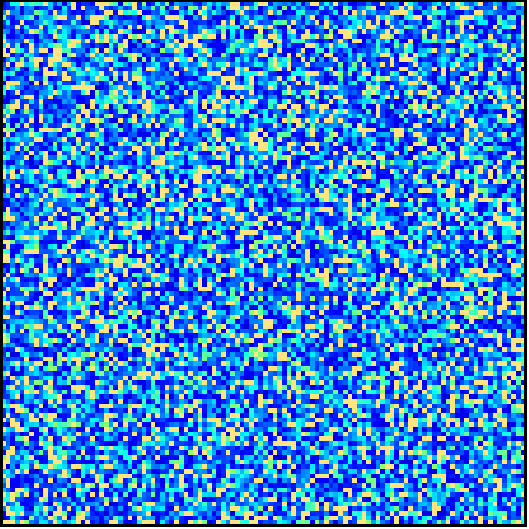
\includegraphics[width=\textwidth, keepaspectratio]{images/ch03/input-matrices/decomposition-benchmarks/Cejka558.pdf}
		\subcaption{Nonzero element pattern of the \textit{Cejka558} matrix.
The plot was generated using a Matlab script that utilizes the CSPY function from \citetitle{RYCUliMIt7YSqfnv} \cite{RYCUliMIt7YSqfnv, Davis2006}.
In the plot, the color of nonzero elements depends on their absolute value.
Small entries are light orange, large entries are black, and the color of mid-range entries ranges from light green to deep blue depending on the median of $\log_{10}$ of the nonzero values (with slight alterations) \cite{Davis2006}.
The color of zero entries is white.}
		\label{Figure:comparing-decomposers-and-solvers->decomposition-project-benchmarks->decomposers-benchmark->comparison-of-execution-times-on-subset-of-matrices->nonzero-element-pattern->Cejka558}
	\end{subfigure}\hspace{0.03\textwidth}
	\begin{subfigure}[t]{0.51\textwidth}
		\centering
		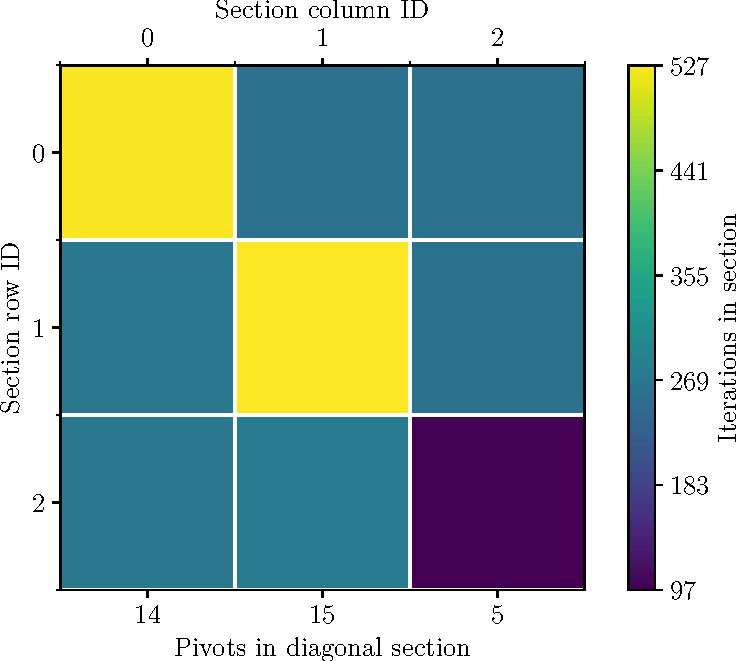
\includegraphics[width=\textwidth, keepaspectratio, clip]{images/ch03/input-matrices/decomposition-benchmarks/Cejka558_icm32pp_metrics.pdf}
		\subcaption{Iterative and pivoting metrics of ICM\_32PP collected during the decomposition of the \textit{Cejka558} matrix.
Each square represents a 256-by-256 section of the matrix.
The color in each square represents the number of iterations performed on that section.
The left and top axes show the section ID in each dimension, while the bottom axis shows the number of pivots performed in a diagonal section.
For example, the number of elements pivoted in section (0,0) was 14, while in section (1,1) it was 15.
The plot was generated using a Python script.}
		\label{Figure:comparing-decomposers-and-solvers->decomposition-project-benchmarks->decomposers-benchmark->comparison-of-execution-times-on-subset-of-matrices->ICMxPP-metrics->Cejka558}
	\end{subfigure}
	\caption{Nonzero element pattern of the \textit{Cejka558} matrix along with the iterative and pivoting metrics of ICM\_32PP.
		The scripts used to generate the plots are available on request or as an attachment to this thesis.
	}
	\label{Figure:comparing-decomposers-and-solvers->decomposition-project-benchmarks->decomposers-benchmark->comparison-of-execution-times-on-subset-of-matrices->matrix-with-metrics->Cejka558}
\end{figure}

As Figure~\ref{Figure:comparing-decomposers-and-solvers->decomposition-project-benchmarks->decomposers-benchmark->comparison-of-execution-times-on-subset-of-matrices->nonzero-element-pattern->Cejka558} shows, there are no zeros in the entire matrix except for some elements on the main diagonal which are not visible.
Furthermore, since the matrix values were randomly generated, there were no patterns that would enable ICM\_32PP to decompose the matrix rapidly.
This is also apparent from Figure~\ref{Figure:comparing-decomposers-and-solvers->decomposition-project-benchmarks->decomposers-benchmark->comparison-of-execution-times-on-subset-of-matrices->ICMxPP-metrics->Cejka558}, where it can be seen that the top-left and center sections were each computed in roughly 527 iterations.

In general, the number of iterations required to process a section of a \textit{Cejka} dense matrix depends on the type of the section.
In the case of a \textit{diagonal section}, the number of iterations can be estimated as $2s + p$, where $s$ represents the size of one dimension of a section and $p$ denotes the number of elements pivoted in the section.
This estimate comes from the observation that the number of iterations depends on the number of diagonal elements in a section.
Specifically, the number of iterations performed per diagonal element varies based on two cases.

The first case assumes that the diagonal element is the bottom-right-most element of the section, and in this case, two iterations are performed.
In the first iteration, the value of the diagonal element is computed.
In the second iteration, the value is recomputed to assure that it has not changed.
Note that the two iterations are performed regardless of whether the element requires pivoting or not.
If it does require pivoting, then the next steps involve processing the lower sections and pivoting the element.

The second case assumes the opposite, i.e., that the diagonal element is not the bottom-right-most element of the diagonal section.
In this case, either two or three iterations are performed:
%
\begin{tight_itemize}
	\item \textit{Two} iterations are performed if the diagonal element does not require pivoting.
In the first iteration, the diagonal element and the elements below it are computed.
In the second iteration, the elements to the right of the diagonal element are computed.
	\item \textit{Three} iterations are performed if the diagonal element requires pivoting.
In such a case, the following occurs:
	\begin{tight_enumerate}
		\item In the first iteration, the diagonal element and the values below it are computed.
		\item Then, the iteration is performed again to assure that the element still requires pivoting and that the values below it are processed, i.e., they can be used for pivoting.
		\item The lower sections are then processed and the diagonal element is pivoted.
		\item In the third iteration, the elements to the right of the diagonal element are computed.
	\end{tight_enumerate}
\end{tight_itemize}

Additionally, if the diagonal section is the top-left section of the matrix, then the estimate is adjusted to $2s + p - 1$ since the first column of \code{LU} is the same as \code{A}.
Therefore, in the first iteration, the values in the first column are already processed, which leads to the values to the right of the first diagonal element being finalized in the first iteration.
Thus, an iteration is saved, hence the adjustment.

Note that in the context of this explanation, the computing of elements only refers to the computation of elements within the diagonal section.

According to the adjusted formula proposed above, the number of iterations required to process the top-left diagonal section of the \textit{Cejka558} matrix is estimated to equal $2\cdot 256 + 14 - 1 = 525$, which corresponds to the number of iterations performed.
Similarly, according to the formula presented earlier ($2s + p$), the number of iterations required to process the center section was 527, which corresponds to the number of iterations performed.\\
In the case of the bottom-right diagonal section, the formula must be offset to account for the matrix bounds.
For example, when considering the 558-by-558 matrix \textit{Cejka558}, since each section represents a 256-by-256 block of elements, the bottom-right diagonal section would extend beyond the bounds of the matrix.
Therefore, its boundaries are adjusted to match the boundaries of the matrix, resulting in a 46-by-46 block of elements.
The processing of this section is expected to require $2\cdot 46 + 5 = 97$ iterations.
As shown in Figure~\ref{Figure:comparing-decomposers-and-solvers->decomposition-project-benchmarks->decomposers-benchmark->comparison-of-execution-times-on-subset-of-matrices->ICMxPP-metrics->Cejka558}, this estimate is correct.

Continuing the context of the \textit{Cejka} dense matrices, the number of iterations required to process a \textit{lower section} is estimated to equal $s + p$, where $s$ represents the size of one dimension of a section and $p$ denotes the number of elements pivoted in the diagonal section above the lower section.
Specifically, the number of iterations corresponds to the number of columns the section encompasses and the number of elements pivoted in the diagonal section above as described below:
%
\begin{tight_itemize}
	\item \textit{Number of columns} - This is due to the chain of dependencies of each element.
		In other words, for a value in the lower section to be computed, it depends on the values to its left and the values in its column above the main diagonal.
		Since the latter are processed before the computation of the lower section begins, only the values to the left of the element remain to be processed.
		In the first iteration on a lower section, the values in the first column are processed.
		To clarify, in the first iteration, multiple columns of values in the section are computed, however, only the values in the first column are processed, i.e., their values are finalized in the first iteration.
		In the second iteration, the values in the second column are processed as they depend on the values processed in the first iteration.
		In summary, with each iteration, one column is processed.
	\item \textit{Number of elements pivoted} - The addition of this value stems from the fact that before an element of a diagonal section is pivoted, the sections below the diagonal section are processed until, and including, the column containing the bad element.
		Thus, for every pivoted element, an extra iteration is performed to verify that the values up to and including the column are not changing, i.e., they are processed.
\end{tight_itemize}

Note that even if the lower section is adjusted to fit the boundaries of the matrix, the number of iterations remains the same as the number of columns is not changed.
For example, when considering the \textit{Cejka558} matrix, the sections below the top-left diagonal section were processed in 270 iterations, which aligns with the prediction mentioned earlier: $256 + 14$.
Similarly, the section below the center diagonal section was processed in 272 iterations, while the prediction was 271.

The prediction of the number of iterations required to process a \textit{right section} is similar to that of a lower section, except for the pivoting aspect.
In other words, the number of iterations required to process a right section is estimated to equal $s + 1$, where $s$ represents the number of rows the section encompasses.
The additional iteration is performed to assure that the values of the right section are not changing, i.e., that they are processed.
Similarly to the lower sections, the number of iterations required to process a right section is not affected if the section is adjusted to fit the boundaries of the matrix.
For example, in the context of the \textit{Cejka558} matrix, all right sections were processed in 257 iterations, which aligns with the prediction.

To show that the prediction is valid for other \textit{Cejka} matrices, the iterative and pivoting metrics for ICM\_32PP are presented in Figure~\ref{Figure:comparing-decomposers-and-solvers->decomposition-project-benchmarks->decomposers-benchmark->comparison-of-execution-times-on-subset-of-matrices->ICMxPP-metrics->Cejka3839-and-Cejka10135} for matrices \textit{Cejka3839} and \textit{Cejka10135}.

\begin{figure}[ht!]
	\centering
	\begin{subfigure}[t]{0.48\textwidth}
		\centering
		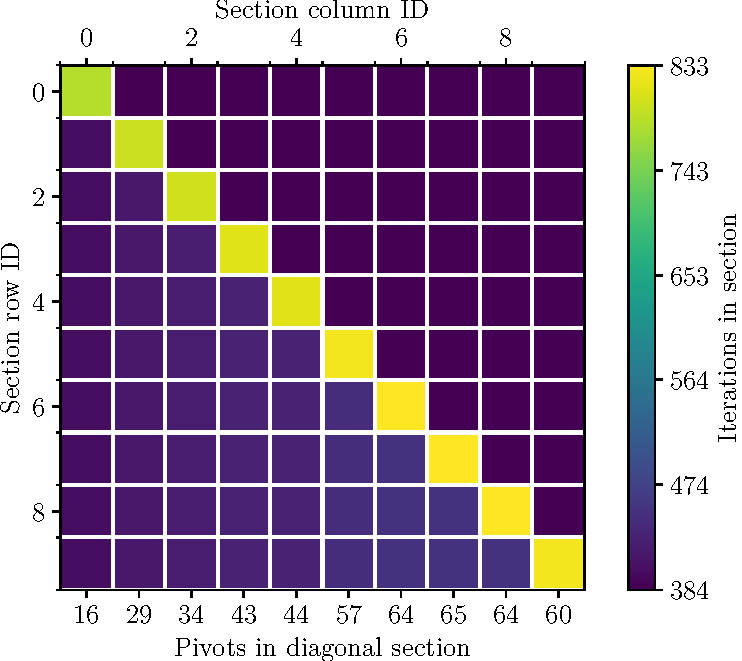
\includegraphics[width=\textwidth, keepaspectratio]{images/ch03/input-matrices/decomposition-benchmarks/Cejka3839_icm32pp_metrics.pdf}
		\subcaption{Iterative and pivoting metrics of ICM\_32PP collected during the decomposition of the \textit{Cejka3839} matrix.
Each square represents a 384-by-384 section of the matrix.}
		\label{Figure:comparing-decomposers-and-solvers->decomposition-project-benchmarks->decomposers-benchmark->comparison-of-execution-times-on-subset-of-matrices->ICMxPP-metrics->Cejka3839}
	\end{subfigure}\hspace{0.03\textwidth}
	\begin{subfigure}[t]{0.48\textwidth}
		\centering
		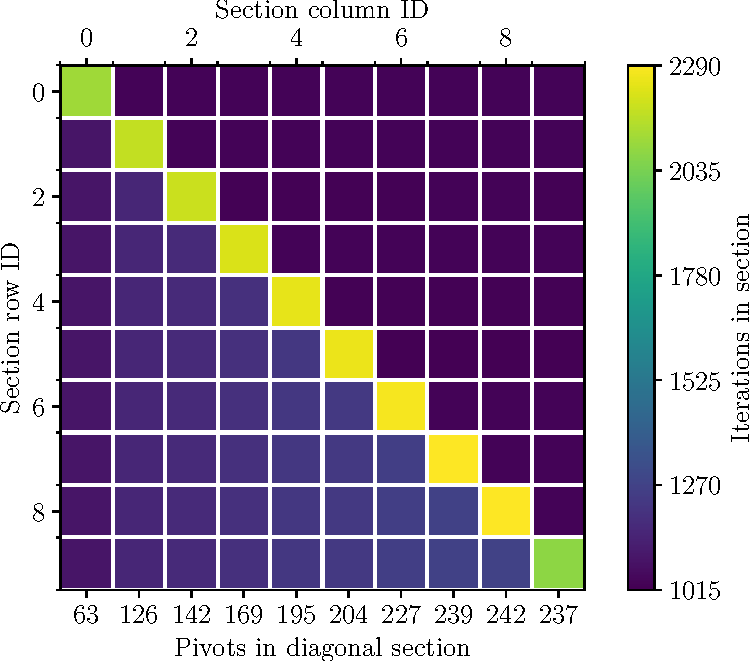
\includegraphics[width=\textwidth, keepaspectratio, clip]{images/ch03/input-matrices/decomposition-benchmarks/Cejka10135_icm32pp_metrics.pdf}
		\subcaption{Iterative and pivoting metrics of ICM\_32PP collected during the decomposition of the \textit{Cejka10135} matrix.
Each square represents a 1024-by-1024 section of the matrix.}
		\label{Figure:comparing-decomposers-and-solvers->decomposition-project-benchmarks->decomposers-benchmark->comparison-of-execution-times-on-subset-of-matrices->ICMxPP-metrics->Cejka10135}
	\end{subfigure}
	\caption{Iterative and pivoting metrics of ICM\_32PP collected during the decomposition of the \textit{Cejka3839} and \textit{Cejka10135} matrices.}
	\label{Figure:comparing-decomposers-and-solvers->decomposition-project-benchmarks->decomposers-benchmark->comparison-of-execution-times-on-subset-of-matrices->ICMxPP-metrics->Cejka3839-and-Cejka10135}
\end{figure}

For example, in the case of \textit{Cejka3839}, each right section took between 384 and 385 iterations to process, whereas the right sections of the \textit{Cejka10135} matrix were processed in 1024 to 1025 iterations.
The prediction for the former yields $384 + 1 = 385$ and the prediction for the latter yields $1024 + 1 = 1025$.
Note that the difference in one iteration is most likely caused by the values of two columns being finalized in one iteration due to a favorable pattern.
In Figures~\ref{Figure:comparing-decomposers-and-solvers->decomposition-project-benchmarks->decomposers-benchmark->comparison-of-execution-times-on-subset-of-matrices->ICMxPP-metrics->Cejka3839} and \ref{Figure:comparing-decomposers-and-solvers->decomposition-project-benchmarks->decomposers-benchmark->comparison-of-execution-times-on-subset-of-matrices->ICMxPP-metrics->Cejka10135}, it can be observed that the colors of the diagonal and lower sections become lighter as the number of elements pivoted in each diagonal section increases.
The only exception to this color lightening is the bottom-right-most diagonal section of the \textit{Cejka10135} matrix.
Similarly to the case with the last diagonal section of the \textit{Cejka558} matrix, the section was adjusted to match the boundaries of the matrix.
Therefore, instead of being a 1024-by-1024 section, it became a 919-by-919 section, requiring $2\cdot 919 + 237 = 2075$ iterations to process.

Dense matrices with randomly generated values offer practically negligible opportunities for ICM\_\textit{x}PP to skip the computation of elements.
Therefore, such matrices represent the worst-case scenario for the ICM\_\textit{x}PP decomposer, and the formulas derived from their decompositions can be considered as an inclusive upper bound estimate of the number of iterations required to process a section.
In summary, for dense matrices with randomly-generated values, ICM\_\textit{x}PP effectively becomes an inefficient adaption of PCM\_\textit{x}PP.

Steering away from instances of poor performance by ICM\_\textit{x}PP, there were three notable matrices out of the subset of 15 where ICM\_\textit{x}PP outperformed PCM\_\textit{x}PP using both double and single precision: \textit{poc-24\_2\_2}, \textit{poc-32\_2\_2}, and \textit{c-22}.
In general, it can be argued that ICM\_\textit{x}PP outperformed PCM\_\textit{x}PP on the aforementioned matrices, as they required minimal, if any, pivoting.
Seeing as the matrices prefixed with \textit{poc} were obtained from the "Poisson equation on a cube" problem implemented in BDDCML, they are discussed as part of Section~\ref{Section:comparing-decomposers-and-solvers->bddcml-benchmark}.

When using double precision, the best-performing variant of ICM\_\textit{x}PP, ICM\_32PP, decomposed the \textit{c-22} matrix in 1.313 seconds, while the best-performing variant of PCM\_\textit{x}PP, PCM\_8PP, decomposed it in 2.192 seconds.
When single precision was used, ICM\_32PP decomposed the matrix in 0.830 seconds, while PCM\_8PP decomposed it in 0.917 seconds.
The main reason why ICM\_\textit{x}PP performed well specifically on the \textit{c-22} matrix is that the initial estimate, \code{A}, allowed for the majority of the sections to be processed in one iteration, as shown in Figure~\ref{Figure:comparing-decomposers-and-solvers->decomposition-project-benchmarks->decomposers-benchmark->comparison-of-execution-times-on-subset-of-matrices->matrix->c-22}.
To provide context for the iterative metrics, the nonzero element pattern of \code{LU} is presented in Figure~\ref{Figure:comparing-decomposers-and-solvers->decomposition-project-benchmarks->decomposers-benchmark->comparison-of-execution-times-on-subset-of-matrices->matrix->c-22->icmxpp-LU-nonzero-element-pattern}.

\begin{figure}[ht!]
	\centering
	\begin{subfigure}[t]{0.45\textwidth}
		\centering
		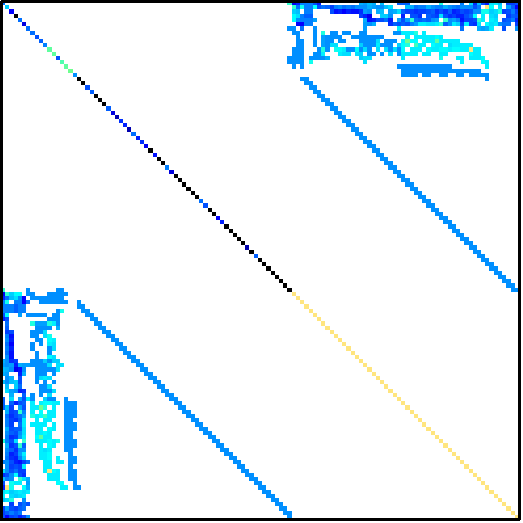
\includegraphics[width=\textwidth, keepaspectratio]{images/ch03/input-matrices/decomposition-benchmarks/c-22.pdf}
		\subcaption{Nonzero element pattern of the \textit{c-22} matrix.}
		\label{Figure:comparing-decomposers-and-solvers->decomposition-project-benchmarks->decomposers-benchmark->comparison-of-execution-times-on-subset-of-matrices->matrix->c-22->nonzero-element-pattern}
	\end{subfigure}\hspace{0.03\textwidth}
	\begin{subfigure}[t]{0.51\textwidth}
		\centering
		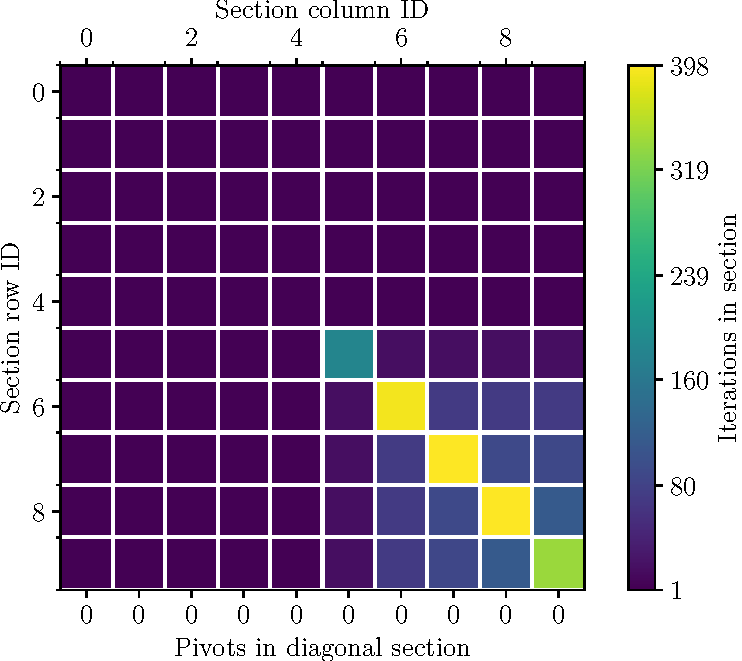
\includegraphics[width=\textwidth, keepaspectratio, clip]{images/ch03/input-matrices/decomposition-benchmarks/c-22_icm32pp_metrics.pdf}
		\subcaption{Iterative and pivoting metrics of ICM\_32PP collected during the decomposition of the \textit{c-22} matrix.
			Each square represents a 384-by-384 section of the matrix.
		}
		\label{Figure:comparing-decomposers-and-solvers->decomposition-project-benchmarks->decomposers-benchmark->comparison-of-execution-times-on-subset-of-matrices->matrix->c-22->icmxpp-metrics}
	\end{subfigure}
	\caption{Nonzero element pattern of the \textit{c-22} matrix along with the iterative and pivoting metrics of ICM\_32PP.
		In the metrics plot, the color in each square represents the number of iterations performed on that section.
		The left and top axes show the section ID in each dimension, while the bottom axis shows the number of pivots performed in a diagonal section.
		However, since no elements were pivoted, the values are all zero.
	}
	\label{Figure:comparing-decomposers-and-solvers->decomposition-project-benchmarks->decomposers-benchmark->comparison-of-execution-times-on-subset-of-matrices->matrix->c-22}
\end{figure}

\begin{figure}[ht!]
	\centering
	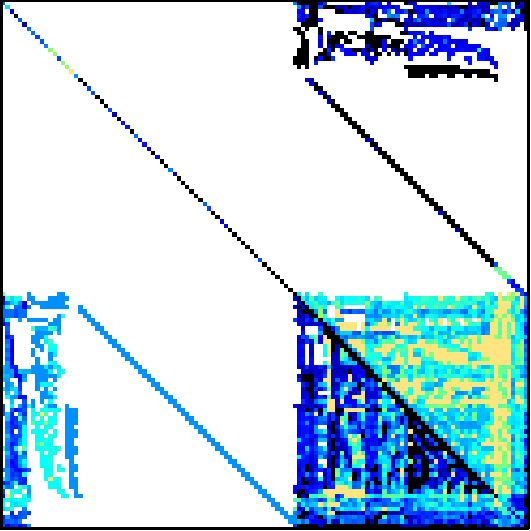
\includegraphics[width=0.45\textwidth, keepaspectratio, clip]{images/ch03/input-matrices/decomposition-benchmarks/c-22_icm32pp.pdf}
	\caption{Nonzero element pattern of the \code{LU} matrix produced by ICM\_32PP through the decomposition of the \textit{c-22} matrix.}
	\label{Figure:comparing-decomposers-and-solvers->decomposition-project-benchmarks->decomposers-benchmark->comparison-of-execution-times-on-subset-of-matrices->matrix->c-22->icmxpp-LU-nonzero-element-pattern}
\end{figure}

As Figure~\ref{Figure:comparing-decomposers-and-solvers->decomposition-project-benchmarks->decomposers-benchmark->comparison-of-execution-times-on-subset-of-matrices->matrix->c-22->nonzero-element-pattern} shows, the main diagonal comprises nonzero elements.
Therefore, the conditional partial pivoting of ICM\_\textit{x}PP was not required.
Furthermore, according to the iterative metrics in Figure~\ref{Figure:comparing-decomposers-and-solvers->decomposition-project-benchmarks->decomposers-benchmark->comparison-of-execution-times-on-subset-of-matrices->matrix->c-22->icmxpp-metrics} and the resulting \code{LU} matrix shown in Figure~\ref{Figure:comparing-decomposers-and-solvers->decomposition-project-benchmarks->decomposers-benchmark->comparison-of-execution-times-on-subset-of-matrices->matrix->c-22->icmxpp-LU-nonzero-element-pattern}, it can be seen that all sections until section (5, 5) took only one iteration to process.
Thus, as mentioned before, the initial estimate of \code{LU} in the form of \code{A}, described in Section~\ref{Subsection:implementation->decomposition-project->implemented-solutions->decomposers}, was instrumental in the efficient decomposition of the \textit{c-22} matrix.
In this case, the initial estimate was suitable since the input matrix mainly had elements on the main diagonal.
Therefore, ICM\_\textit{x}PP used the elements of the main diagonal of \code{A} in the main diagonal of \code{L}.
Then, the multiplication of \code{L} and \code{U}, which has a unit diagonal, essentially meant that \code{L} was multiplied by a matrix resembling the identity matrix.
As the figures further show, the elements in the bottom-left and top-right of \code{LU} disrupted the simple computation of the main diagonal.
Subsequently, the bottom-right part of \code{LU} required many iterations to account for the disturbance.
The claim that ICM\_\textit{x}PP performs well on matrices with most of their nonzero elements on the main diagonal corresponds to the findings presented in Chapter 3 of \citetitle{Cejka2022} \cite{Cejka2022}.

Next, the variants of ICM\_\textit{x}PP will be compared to each other.
While Figure~\ref{Figure:comparing-decomposers-and-solvers->decomposition-project-benchmarks->decomposers-benchmark->comparison-of-execution-times-on-subset-of-matrices->precisions} presents the execution times of all variants of ICM\_\textit{x}PP, it may be difficult to discern the differences in performance.
Thus, to compare the performance of the variants of ICM\_\textit{x}PP, Figure~\ref{Figure:comparing-decomposers-and-solvers->decomposition-project-benchmarks->decomposers-benchmark->comparison-of-execution-times-on-subset-of-matrices->ICMxPP-double-precision} shows their execution times on the subset of matrices when double precision was used.
Note that unlike in Figure~\ref{Figure:comparing-decomposers-and-solvers->decomposition-project-benchmarks->decomposers-benchmark->comparison-of-execution-times-on-subset-of-matrices->precisions}, the vertical axis in Figure~\ref{Figure:comparing-decomposers-and-solvers->decomposition-project-benchmarks->decomposers-benchmark->comparison-of-execution-times-on-subset-of-matrices->ICMxPP-double-precision} is not log-scaled to better portray the differences in performance among the variants.

\begin{figure}[ht!]
	\centering
	\tikzset{mark options={mark size=2.0, line width=0.5pt},font=\small}
	\begin{tikzpicture}
		\pgfplotstableread[col sep=comma]{resources/ch03/decomposition-benchmarks/decomposers/15-pivoting-matrices-double-precision.csv}\datatable
		\begin{axis}
			[
			,width=\textwidth
			,height=0.45\textwidth
			,axis x line*=bottom
			,axis y line*=left
			,xlabel=\textbf{Matrix}
			,x label style={at={(axis description cs:0.575,-0.35)}}
			,ylabel={\textbf{Execution time [s]}}
			,xmin=-.5, xmax=14.5
			,xtick=data
			,xticklabels={poc-8\_4\_2-1,Cejka558,poc-24\_2\_2,Cejka2599,poc-32\_2\_2,c-22,Cejka4156,freeFlyingRobot\_9,Cejka6574,fp,Cejka8385,nd3k,Cejka10135,msc10848,sinc15}
			,x tick label style={rotate=45,anchor=east,yshift=-6pt,align=right}
			,ymajorgrids
			,legend style={
				at={(0.5,1.025)},
				anchor=south,
				legend columns=4,
				/tikz/every even column/.append style={column sep=0.5cm},
				draw=black, % Remove legend border
				nodes={inner sep=3pt}, % Adjust the spacing between legend entries
				font=\small % Adjust the font size of the legend entries
			}
			]
			\addplot[blue,mark=triangle*] table [x=id, y=ICM_8PP-time] {\datatable};
			\addlegendentry{ICM\_8PP}
			\addplot[purple,mark=triangle*] table [x=id, y=ICM_16PP-time] {\datatable};
			\addlegendentry{ICM\_16PP}
			\addplot[teal,mark=triangle*] table [x=id, y=ICM_32PP-time] {\datatable};
			\addlegendentry{ICM\_32PP}
		\end{axis}
	\end{tikzpicture}	
	\caption{Execution times of the variants of ICM\_\textit{x}PP on the subset of matrices shown in Table~\ref{Table:comparing-decomposers-and-solvers->decomposition-project-benchmarks->matrices-used-for-benchmarks->15-selected-matrices} using double precision.}
	\label{Figure:comparing-decomposers-and-solvers->decomposition-project-benchmarks->decomposers-benchmark->comparison-of-execution-times-on-subset-of-matrices->ICMxPP-double-precision}
\end{figure}

Out of the three variants of ICM\_\textit{x}PP that were benchmarked on the subset of 15 matrices, ICM\_32PP performed the best and ICM\_8PP the worst, as can be seen in Figure~\ref{Figure:comparing-decomposers-and-solvers->decomposition-project-benchmarks->decomposers-benchmark->comparison-of-execution-times-on-subset-of-matrices->ICMxPP-double-precision}.

To determine the reason behind the differences in performance between the variants, it is necessary to consider different aspects of the implementations.
Since the section size is near-identical for all variants, and the difference in the number of threads performing a row swap in each variant does not affect the performance, the only remaining major factor is the kernels computing the iterations.\\
Disregarding the changes in the implementations of the kernels since they were benchmarked in \citetitle{Cejka2022} \cite{Cejka2022}, it can be argued that the difference in the performance of the variants of ICM\_\textit{x}PP is due to uncoalesced and inefficient global memory access.

First, the issue of uncoalesced global memory access will be described.
In the context of the Decomposition benchmark for decomposers, the matrices were stored in row-major order on the GPU for the ICM\_\textit{x}PP decomposer.
As a result, uncoalesced access to global memory occurs for ICM\_8PP and ICM\_16PP.

For example, in the case of ICM\_8PP, this is due to it using 8-by-8 thread blocks.
Since threads consecutive in their 1st dimension are grouped into warps of 32 threads, each block of threads in ICM\_8PP is made up of two warps.
The first warp consists of threads in the first four rows of the thread block, while the remaining threads belong to the second warp.
When these threads read matrix elements from global memory, the first row of eight threads reads neighboring elements, and the next row of threads also reads neighboring elements.
However, the second group of eight elements is not adjacent to the first group of eight elements.
In general, while each group of eight threads within a warp accesses neighboring global memory addresses, the accessed elements of each group are not adjacent to those accessed by the other groups of eight threads.
Therefore, instead of the threads within a warp all reading neighboring elements in parallel, i.e., in one read transaction, they perform $32/8 = 4$ sequential read transactions \cite{Cejka2022}.

Similarly, since ICM\_16PP uses 16-by-16 thread blocks, each warp performs $32/16 = 2$ sequential transactions when reading from global memory during kernel execution.
Conversely, this issue is not present for ICM\_32PP since each row of a thread block comprises one warp of threads.
Thus, the threads of each warp read 32 neighboring elements in one transaction.

The next issue, inefficient global memory access, describes a scenario where the smaller the thread blocks are, the more accesses to global memory they perform.
In Section~\ref{Subsection:implementation->decomposition-project->implemented-solutions->decomposers} the following was mentioned in terms of the computation kernels of ICM\_\textit{x}PP:

\begin{quoting}
\textit{... each block of threads is responsible for computing a block of elements in \code{LUnext}.
Thus, to use shared memory and avoid unnecessary accesses to global memory, the block of threads performs matrix multiplication by iterating over blocks of elements.
In other words, it loads a block of elements from global memory to shared memory, multiplies them, and then moves on to the next block.
The value a thread computes for each block of elements is added to a local variable, \code{sum}.
Matrix multiplication by blocks of elements using shared memory is depicted in Figure~\ref{Figure:implementation->decomposition-project->implemented-solutions->decomposers->ICMxPP->CUDA-matrix-multiplication-with-shared-memory}.}
\end{quoting}

When a block of threads performs matrix multiplication by iterating over blocks of elements, each iteration involves a 32-by-32 block of threads reading from global memory only once.
On the other hand, to cover the same block of elements, 16 8-by-8 blocks of threads are required.
Specifically, four 8-by-8 blocks of threads stacked on top of each other are required to compute eight columns, and there are four parts consisting of eight columns each in 32 columns.
Therefore, in each iteration, the four blocks stacked on top of each other will read the same 8-by-8 block of elements four times in total, since they cannot access the shared memory of the other thread blocks.
This means that when a 32-by-32 block of threads computes the values of a 32-by-32 block of elements in \code{LU}, it performs fewer read operations from global memory compared to using multiple 8-by-8 blocks of threads to compute the same block of elements.

The consequences of these inefficiencies are visible in Figure~\ref{Figure:comparing-decomposers-and-solvers->decomposition-project-benchmarks->decomposers-benchmark->comparison-of-execution-times-on-subset-of-matrices->ICMxPP-double-precision}, where, especially for matrices that take a long time to decompose, ICM\_32PP consistently outperforms ICM\_16PP, which in turn consistently outperforms ICM\_8PP.\label{Text:comparing-decomposers-and-solvers->decomposition-project-benchmarks->decomposers-benchmark->comparison-of-execution-times-on-subset-of-matrices->ICMxPP->performance-of-variants}

\paragraph{CMPP} As can be seen from Figure~\ref{Figure:comparing-decomposers-and-solvers->decomposition-project-benchmarks->decomposers-benchmark->comparison-of-execution-times-on-subset-of-matrices->precisions}, the CMPP decomposer performed worse than the other benchmarked decomposers on all matrices of the subset, except for the \textit{poc-8\_4\_2-1} and \textit{Cejka558} matrices.
The lack of performance can be attributed to two main reasons: the algorithm of CMPP is strictly sequential, and its implementation is not optimized.
The performance of CMPP greatly depends on the dimensions of the input matrix, therefore, only the execution times it achieved on the smallest and largest matrices of the subset will be mentioned.
When using double precision, CMPP decomposed the \textit{poc-8\_4\_2-1} matrix in 0.003 seconds and the \textit{sinc15} matrix in 536.824 seconds.
When using single precision, CMPP decomposed the matrices in 0.003 and 517.045 seconds, respectively.
For context, the slowest variant of ICM\_\textit{x}PP, ICM\_8PP, decomposed the \textit{sinc15} matrix in 494.174 seconds using double precision.
Ultimately, in the context of the Decomposition benchmark for decomposers, CMPP served as a baseline against which other decomposers were expected to perform better.
Additionally, it served as a means to verify the accuracy of results produced by the other decomposers.

\paragraph{PCM\_\textit{x}PP}\label{Paragraph:comparing-decomposers-and-solvers->decomposition-project-benchmarks->decomposers-benchmark->comparison-of-execution-times-on-subset-of-matrices->PCMxPP} Overall, on the subset of 15 matrices, PCM\_\textit{x}PP was the second fastest decomposer.
Since its algorithm is a parallelized version of CMPP's algorithm, its performance also heavily depends on the dimensions of the input matrix, as shown in Figure~\ref{Figure:comparing-decomposers-and-solvers->decomposition-project-benchmarks->decomposers-benchmark->comparison-of-execution-times-on-subset-of-matrices->precisions}.
For the analysis of PCM\_\textit{x}PP, Figure~\ref{Figure:comparing-decomposers-and-solvers->decomposition-project-benchmarks->decomposers-benchmark->comparison-of-execution-times-on-subset-of-matrices->PCMxPP-double-precision} displays the execution times of its variants when double precision was used.

\begin{figure}[ht!]
	\centering
	\tikzset{mark options={mark size=2.0, line width=0.5pt},font=\small}
	\begin{tikzpicture}
		\pgfplotstableread[col sep=comma]{resources/ch03/decomposition-benchmarks/decomposers/15-pivoting-matrices-double-precision.csv}\datatable
		\begin{axis}
			[
			,width=\textwidth
			,height=0.45\textwidth
			,axis x line*=bottom
			,axis y line*=left
			,xlabel=\textbf{Matrix}
			,x label style={at={(axis description cs:0.575,-0.35)}}
			,ylabel={\textbf{Execution time [s]}}
			,xmin=-.5, xmax=14.5
			,xtick=data
			,xticklabels={poc-8\_4\_2-1,Cejka558,poc-24\_2\_2,Cejka2599,poc-32\_2\_2,c-22,Cejka4156,freeFlyingRobot\_9,Cejka6574,fp,Cejka8385,nd3k,Cejka10135,msc10848,sinc15}
			,x tick label style={rotate=45,anchor=east,yshift=-6pt,align=right}
			,ymajorgrids
			,legend style={
				at={(0.5,1.025)},
				anchor=south,
				legend columns=4,
				/tikz/every even column/.append style={column sep=0.5cm},
				draw=black, % Remove legend border
				nodes={inner sep=3pt}, % Adjust the spacing between legend entries
				font=\small % Adjust the font size of the legend entries
			}
			]
			\addplot[red,mark=triangle*] table [x=id, y=PCM_8PP-time] {\datatable};
			\addlegendentry{PCM\_8PP}
			\addplot[nvidia,mark=triangle*] table [x=id, y=PCM_16PP-time] {\datatable};
			\addlegendentry{PCM\_16PP}
			\addplot[cyan,mark=triangle*] table [x=id, y=PCM_32PP-time] {\datatable};
			\addlegendentry{PCM\_32PP}
		\end{axis}
	\end{tikzpicture}	
	\caption{Execution times of the variants of PCM\_\textit{x}PP on the subset of matrices shown in Table~\ref{Table:comparing-decomposers-and-solvers->decomposition-project-benchmarks->matrices-used-for-benchmarks->15-selected-matrices} using double precision.}
	\label{Figure:comparing-decomposers-and-solvers->decomposition-project-benchmarks->decomposers-benchmark->comparison-of-execution-times-on-subset-of-matrices->PCMxPP-double-precision}
\end{figure}

As can be seen in Figure~\ref{Figure:comparing-decomposers-and-solvers->decomposition-project-benchmarks->decomposers-benchmark->comparison-of-execution-times-on-subset-of-matrices->PCMxPP-double-precision}, PCM\_8PP consistently outperforms PCM\_16PP, which in turn consistently outperforms PCM\_32PP.  Similarly to ICM\_\textit{x}PP, the difference in execution times increases with larger matrix dimensions.

In the context of the Decomposition benchmark for decomposers, the input matrix was stored in row-major order, which resulted in slightly lower execution times for the variants compared to when column-major ordering was used.
The higher performance of the decomposer with row-major ordering was unexpected since it meant that accesses to global memory were not coalesced.
As mentioned in Section~\ref{Subsection:implementation->decomposition-project->implemented-solutions->decomposers}, the thread blocks of PCM\_\textit{x}PP are one-dimensional and consist of $x^2$ threads.
In the context of PCM\_32PP, when the threads of a block read a column of elements from global memory in each iteration of the for loop shown in Listing~\ref{Listing:PCMxPP-implementation->kernels->column-compute-kernel}, the addresses accessed by the threads are not adjacent.
As a result, the global memory access of threads belonging to each warp is not coalesced.
This means that the read operations performed by the warp are divided into more memory transactions compared to coalesced global memory access.
Nevertheless, uncoalesced access to global memory did not seem to have a noticeable impact on the performance of PCM\_\textit{x}PP.

The differences in the performance of the variants of PCM\_\textit{x}PP can be attributed to idle resources.
This claim is based on the observation that the execution time of PCM\_32PP and PCM\_16PP consistently appears to be worse than that of PCM\_8PP for larger sparse matrices.
The GPU used for the benchmarks, Nvidia A100, has the following limitations per SM \cite{rfiOEXAGDlcAOxF3}:
%
\begin{tight_enumerate}
	\item maximum threads per SM: 2048,
	\item maximum warps per SM: 64, and
	\item maximum thread blocks per SM: 32.
\end{tight_enumerate}
%
Therefore, the PCM\_32PP decomposer, which uses blocks of 1024 threads, can only schedule two of its blocks per SM before the threads-per-SM limit is reached.
Moreover, a block of threads cannot be released from an SM until all of its warps have completed their work \cite{Cheng2014}.
Consequently, if one warp within the block takes longer to complete its work, it can potentially hold the entire block of 1024 threads in the SM, preventing the scheduling of another thread block.
This situation results in idle resources on the SM, as the other warps have already completed their work.
Notably, this scenario is more likely to occur with blocks consisting of a larger number of threads.

This congestion is less likely to occur for blocks with fewer threads since each SM can handle more blocks simultaneously.
For example, PCM\_16PP, which uses blocks of 256 threads, can schedule up to eight of its blocks per SM.
Similarly, PCM\_8PP can schedule up to 32 of its blocks, each consisting of 64 threads, per SM.

Earlier, it was mentioned that this behavior can be observed for larger sparse matrices.
This is due to larger matrices generally requiring more computing threads, thus necessitating more thread blocks.
Furthermore, the sparsity of the matrices increases the likelihood of an unequal distribution of work across warps, as the majority of elements are zero.
In other words, during the decomposition of sparse matrices, it is more likely for many warps to be working with zeros while other warps are working with nonzeros, which results in the latter requiring more time and causing the idleness of resources.

This behavior seems to occur in Figure~\ref{Figure:comparing-decomposers-and-solvers->decomposition-project-benchmarks->decomposers-benchmark->comparison-of-execution-times-on-subset-of-matrices->PCMxPP-double-precision}, where the execution time of PCM\_32PP appears to spike for larger sparse matrices such as \textit{nd3k} and \textit{msc10848}.
Additionally, the figure shows that the PCM\_16PP decomposer also exhibits a noticeable spike in execution time for the \textit{msc10848} sparse matrix.
In contrast, the PCM\_8PP decomposer, which employs smaller thread blocks compared to the other variants, shows the best performance.

It should be noted once again that the implementation of PCM\_\textit{x}PP was not optimized in any way.
This means that optimization techniques such as shared memory usage, block-level loop unrolling, and others were not employed.
Consequently, as mentioned in Section~\ref{Subsection:implementation->decomposition-project->implemented-solutions->decomposers}, PCM\_\textit{x}PP is highly inefficient and fails to fully exploit the computational power of the GPU.
However, despite its lack of optimization, PCM\_\textit{x}PP still demonstrates better performance compared to the complex implementation of ICM\_\textit{x}PP.
This suggests that ICM\_\textit{x}PP may be suitable for specific types of matrices, such as those encountered in the BDDCML benchmark discussed in Section~\ref{Section:comparing-decomposers-and-solvers->bddcml-benchmark}.

\paragraph{Performance Comparison Relative to CuSolverDnXgetrfPP}\label{Paragraph:comparing-decomposers-and-solvers->decomposition-project-benchmarks->decomposers-benchmark->comparison-of-execution-times-on-subset-of-matrices->performance-comparison-relative->to-CuSolverDnXgetrfPP} For completeness, this section presents the performance comparison of the decomposers listed in Table~\ref{Table:comparing-decomposers-and-solvers->decomposition-project-benchmarks->decomposers-benchmark->table-of-decomposers} relative to the CuSolverDnXgetrfPP decomposer.
First, the speedup relative to the CuSolverDnXgetrfPP decomposer, using both double and single precision, is presented in Figure~\ref{Figure:comparing-decomposers-and-solvers->decomposition-project-benchmarks->decomposers-benchmark->comparison-of-execution-times-on-subset-of-matrices->performance-comparison-relative->to-CuSolverDnXgetrfPP->speedup-comparison-with-other-decomposers}.
Then, the execution times of the decomposers for both double and single precision are presented in Tables~\ref{Table:comparing-decomposers-and-solvers->decomposition-project-benchmarks->decomposers-benchmark->comparison-of-execution-times-on-subset-of-matrices->execution-times->double-precision} and \ref{Table:comparing-decomposers-and-solvers->decomposition-project-benchmarks->decomposers-benchmark->comparison-of-execution-times-on-subset-of-matrices->execution-times->single-precision}, respectively.
Note that the tables only show the execution times of the best-performing variants of ICM\_\textit{x}PP and PCM\_\textit{x}PP.

% Speedup of decomposers relative to CuSolverDnXgetrfPP
\begin{figure}[ht!]
	\centering
	\tikzset{mark options={mark size=2.0, line width=0.5pt},font=\small}
	\begin{subfigure}{\textwidth}
		\begin{tikzpicture}
			\pgfplotstableread[col sep=comma]{resources/ch03/decomposition-benchmarks/decomposers/15-pivoting-matrices-double-precision.csv}\datatable
			\begin{axis}
				[
				,width=\textwidth
				,height=0.45\textwidth
				,axis x line*=bottom
				,axis y line*=left
				,xlabel=\textbf{Matrix}
				,x label style={at={(axis description cs:0.575,-0.35)}}
				,ylabel=\textbf{Speedup} ($\log$-scaled)
				,xmin=-.5, xmax=14.5
				,ymode=log
				,xtick=data
				,xticklabels={poc-8\_4\_2-1,Cejka558,poc-24\_2\_2,Cejka2599,poc-32\_2\_2,c-22,Cejka4156,freeFlyingRobot\_9,Cejka6574,fp,Cejka8385,nd3k,Cejka10135,msc10848,sinc15}
				,x tick label style={rotate=45,anchor=east,yshift=-6pt,align=right}
				,ymajorgrids
				,legend style={
					at={(0.5,1.025)},
					anchor=south,
					legend columns=4,
					/tikz/every even column/.append style={column sep=0.5cm},
					draw=black, % Remove legend border
					nodes={inner sep=3pt}, % Adjust the spacing between legend entries
					font=\small % Adjust the font size of the legend entries
				}
				]
				\addplot[black,mark=triangle*] table [x=id, y=CMPP-speedup] {\datatable};
				\addlegendentry{CMPP}
				\addplot[blue,mark=triangle*] table [x=id, y=ICM_8PP-speedup] {\datatable};
				\addlegendentry{ICM\_8PP}
				\addplot[purple,mark=triangle*] table [x=id, y=ICM_16PP-speedup] {\datatable};
				\addlegendentry{ICM\_16PP}
				\addplot[teal,mark=triangle*] table [x=id, y=ICM_32PP-speedup] {\datatable};
				\addlegendentry{ICM\_32PP}
				\addplot[green!60!black,mark=none,style={ultra thick}] table [x=id, y=CuSolverDnXgetrfWrapperPP-speedup] {\datatable};
				\addlegendentry{CuSolverDnXgetrfPP}
				\addplot[red,mark=triangle*] table [x=id, y=PCM_8PP-speedup] {\datatable};
				\addlegendentry{PCM\_8PP}
				\addplot[nvidia,mark=triangle*] table [x=id, y=PCM_16PP-speedup] {\datatable};
				\addlegendentry{PCM\_16PP}
				\addplot[cyan,mark=triangle*] table [x=id, y=PCM_32PP-speedup] {\datatable};
				\addlegendentry{PCM\_32PP}
			\end{axis}
		\end{tikzpicture}
		\subcaption{Double precision}
		\label{Figure:comparing-decomposers-and-solvers->decomposition-project-benchmarks->decomposers-benchmark->comparison-of-execution-times-on-subset-of-matrices->performance-comparison-relative->to-CuSolverDnXgetrfPP->speedup-comparison-with-other-decomposers->double-precision}
	\end{subfigure}
	\begin{subfigure}{\textwidth}
		\begin{tikzpicture}
			\pgfplotstableread[col sep=comma]{resources/ch03/decomposition-benchmarks/decomposers/15-pivoting-matrices-single-precision.csv}\datatable
			\begin{axis}
				[
				,width=\textwidth
				,height=0.45\textwidth
				,axis x line*=bottom
				,axis y line*=left
				,xlabel=\textbf{Matrix}
				,x label style={at={(axis description cs:0.575,-0.35)}}
				,ylabel=\textbf{Speedup} ($\log$-scaled)
				,xmin=-.5, xmax=14.5
				,ymode=log
				,xtick=data
				,xticklabels={poc-8\_4\_2-1,Cejka558,poc-24\_2\_2,Cejka2599,poc-32\_2\_2,c-22,Cejka4156,freeFlyingRobot\_9,Cejka6574,fp,Cejka8385,nd3k,Cejka10135,msc10848,sinc15}
				,x tick label style={rotate=45,anchor=east,yshift=-6pt,align=right}
				,ymajorgrids
				]
				\addplot[black,mark=none] table [x=id, y=CMPP-speedup] {\datatable};
				\addplot[blue,mark=triangle*] table [x=id, y=ICM_8PP-speedup] {\datatable};
				\addplot[purple,mark=triangle*] table [x=id, y=ICM_16PP-speedup] {\datatable};
				\addplot[teal,mark=triangle*] table [x=id, y=ICM_32PP-speedup] {\datatable};
				\addplot[green!60!black,mark=none,style={ultra thick}] table [x=id, y=CuSolverDnXgetrfWrapperPP-speedup] {\datatable};
				\addplot[red,mark=triangle*] table [x=id, y=PCM_8PP-speedup] {\datatable};
				\addplot[nvidia,mark=triangle*] table [x=id, y=PCM_16PP-speedup] {\datatable};
				\addplot[cyan,mark=triangle*] table [x=id, y=PCM_32PP-speedup] {\datatable};
			\end{axis}
		\end{tikzpicture}
		\subcaption{Single precision}
		\label{Figure:comparing-decomposers-and-solvers->decomposition-project-benchmarks->decomposers-benchmark->comparison-of-execution-times-on-subset-of-matrices->performance-comparison-relative->to-CuSolverDnXgetrfPP->speedup-comparison-with-other-decomposers->single-precision}
	\end{subfigure}
	\caption{Speedup comparison of the decomposers listed in Table~\ref{Table:comparing-decomposers-and-solvers->decomposition-project-benchmarks->decomposers-benchmark->table-of-decomposers} relative to CuSolverDnXgetrfPP on the subset of matrices shown in Table~\ref{Table:comparing-decomposers-and-solvers->decomposition-project-benchmarks->matrices-used-for-benchmarks->15-selected-matrices} using double and single precision.
		The vertical axis is log-scaled for improved visibility of differences between implementations.
	}
	\label{Figure:comparing-decomposers-and-solvers->decomposition-project-benchmarks->decomposers-benchmark->comparison-of-execution-times-on-subset-of-matrices->performance-comparison-relative->to-CuSolverDnXgetrfPP->speedup-comparison-with-other-decomposers}
\end{figure}

\begin{table}[ht!]
	\centering
	\begin{tabular}{|l|r|r|r|r|}
		\hline
		\rowcolor[HTML]{C0C0C0} \multicolumn{1}{|c|}{\textbf{Matrix}} & \multicolumn{1}{c|}{\textbf{CuSolverDnXgetrfPP}} & \multicolumn{1}{c|}{\textbf{CMPP}} & \multicolumn{1}{c|}{\textbf{ICM\_32PP}} & \multicolumn{1}{c|}{\textbf{PCM\_8PP}} \\ \hline
		poc-8\_4\_2-1      & 0.0012 &    0.0026 &   0.0028 &  0.0079 \\
		Cejka558           & 0.0025 &    0.0431 &   0.1536 &  0.0328 \\
		poc-24\_2\_2       & 0.0089 &    1.6072 &   0.1233 &  0.2498 \\
		Cejka2599          & 0.0138 &    4.9971 &   2.5359 &  0.7432 \\
		poc-32\_2\_2       & 0.0172 &   10.0834 &   0.3185 &  1.4109 \\
		c-22               & 0.0211 &   17.0976 &   1.3125 &  2.1916 \\
		Cejka4156          & 0.0252 &   22.8199 &   9.3951 &  2.7534 \\
		freeFlyingRobot\_9 & 0.0309 &   39.4910 &   7.5774 &  3.7317 \\
		Cejka6574          & 0.0536 &  102.0215 &  48.6333 &  7.3379 \\
		fp                 & 0.0613 &  149.0108 &  10.3767 & 10.0030 \\
		Cejka8385          & 0.0692 &  250.6601 & 123.9475 & 12.6962 \\
		nd3k               & 0.0728 &  261.3578 & 108.3278 & 13.9076 \\
		Cejka10135         & 0.0981 & 1282.0280 & 243.4973 & 18.8531 \\
		msc10848           & 0.1037 &  653.4609 & 231.3460 & 20.6770 \\
		sinc15             & 0.1237 &  536.8241 & 290.3724 & 24.3491 \\ \hline
	\end{tabular}
	\caption{Execution times (in seconds) of the decomposers listed in Table~\ref{Table:comparing-decomposers-and-solvers->decomposition-project-benchmarks->decomposers-benchmark->table-of-decomposers} on the set of matrices (Table~\ref{Table:comparing-decomposers-and-solvers->decomposition-project-benchmarks->matrices-used-for-benchmarks->15-selected-matrices}) using \textit{double} precision.
		Only the execution times of the best-performing variants of ICM\_\textit{x}PP and PCM\_\textit{x}PP are presented.
	}
	\label{Table:comparing-decomposers-and-solvers->decomposition-project-benchmarks->decomposers-benchmark->comparison-of-execution-times-on-subset-of-matrices->execution-times->double-precision}
\end{table}

\begin{table}[ht!]
	\centering
	\begin{tabular}{|l|r|r|r|r|}
		\hline
		\rowcolor[HTML]{C0C0C0} \multicolumn{1}{|c|}{\textbf{Matrix}} & \multicolumn{1}{c|}{\textbf{CuSolverDnXgetrfPP}} & \multicolumn{1}{c|}{\textbf{CMPP}} & \multicolumn{1}{c|}{\textbf{ICM\_32PP}} & \multicolumn{1}{c|}{\textbf{PCM\_8PP}} \\ \hline
		poc-8\_4\_2-1      & 0.0012 &   0.0028 &   0.0021 &  0.0065 \\
		Cejka558           & 0.0024 &   0.0441 &   0.1347 &  0.0244 \\
		poc-24\_2\_2       & 0.0079 &   1.6099 &   0.0684 &  0.1509 \\
		Cejka2599          & 0.0120 &   4.8680 &   1.8898 &  0.2926 \\
		poc-32\_2\_2       & 0.0221 &   8.7752 &   0.1594 &  0.4945 \\
		c-22               & 0.0199 &  15.2680 &   0.8297 &  0.9173 \\
		Cejka4156          & 0.0210 &  21.4828 &   6.4306 &  1.2250 \\
		freeFlyingRobot\_9 & 0.0276 &  36.1487 &   5.1294 &  1.7961 \\
		Cejka6574          & 0.0412 &  90.2590 &  32.6642 &  3.7836 \\
		fp                 & 0.0546 & 159.8940 &   6.0036 &  5.0968 \\
		Cejka8385          & 0.0727 & 276.4194 &  82.7072 &  6.2676 \\
		nd3k               & 0.0834 & 225.9154 &  70.8304 &  7.4513 \\
		Cejka10135         & 0.0859 & 374.2370 & 162.5578 &  9.5356 \\
		msc10848           & 0.0917 & 481.6722 & 155.3406 & 11.6422 \\
		sinc15             & 0.1075 & 517.0449 &        - & 12.6665 \\ \hline
	\end{tabular}
	\caption{Execution times (in seconds) of the decomposers listed in Table~\ref{Table:comparing-decomposers-and-solvers->decomposition-project-benchmarks->decomposers-benchmark->table-of-decomposers} on the set of matrices (Table~\ref{Table:comparing-decomposers-and-solvers->decomposition-project-benchmarks->matrices-used-for-benchmarks->15-selected-matrices}) using \textit{single} precision.
		Only the execution times of the best-performing variants of ICM\_\textit{x}PP and PCM\_\textit{x}PP are presented.
		The execution time of ICM\_32PP is missing for the \textit{sinc15} matrix as ICM\_\textit{x}PP failed to decompose the matrix using single precision.
	}
	\label{Table:comparing-decomposers-and-solvers->decomposition-project-benchmarks->decomposers-benchmark->comparison-of-execution-times-on-subset-of-matrices->execution-times->single-precision}
\end{table}

Figure~\ref{Figure:comparing-decomposers-and-solvers->decomposition-project-benchmarks->decomposers-benchmark->comparison-of-execution-times-on-subset-of-matrices->performance-comparison-relative->to-CuSolverDnXgetrfPP->speedup-comparison-with-other-decomposers}, and Tables~\ref{Table:comparing-decomposers-and-solvers->decomposition-project-benchmarks->decomposers-benchmark->comparison-of-execution-times-on-subset-of-matrices->execution-times->double-precision} and \ref{Table:comparing-decomposers-and-solvers->decomposition-project-benchmarks->decomposers-benchmark->comparison-of-execution-times-on-subset-of-matrices->execution-times->single-precision} suggest that CuSolverDnXgetrfPP is the fastest decomposer among those benchmarked in the Decomposition benchmark for decomposers.
However, the results presented only compare the decomposers on a subset of 15 matrices.
To provide further support for the claim, it is necessary to evaluate the performance of CuSolverDnXgetrfPP on the entire set of 50 matrices.


\subsubsection{Comparison of Execution Times on All Matrices}
This section presents a comparison of the execution times of the decomposers listed in Table~\ref{Table:comparing-decomposers-and-solvers->decomposition-project-benchmarks->decomposers-benchmark->table-of-decomposers} on the set of 50 matrices using both double and single precision.
The benchmarks were run on the platform specified in Section~\ref{Subsection:comparing-decomposers-and-solvers->decomposition-project-benchmarks->benchmark-platform-specifications}.
Similarly to the benchmark results presented in Section~\ref{Subsection:comparing-decomposers-and-solvers->decomposition-project-benchmarks->decomposers-benchmark->comparison-of-execution-times-on-subset-of-matrices}, the matrices were sorted according to their dimensions from smallest to largest.
The execution times are presented in Figure~\ref{Figure:comparing-decomposers-and-solvers->decomposition-project-benchmarks->decomposers-benchmark->comparison-of-execution-time-on-all-matrices->double-and-single-precision}.

\begin{figure}[ht!]
	\centering
	\tikzset{mark options={mark size=1.5},font=\small}
	\begin{subfigure}{\textwidth}
		\begin{tikzpicture}
			\pgfplotstableread[col sep=comma]{resources/ch03/decomposition-benchmarks/decomposers/50-pivoting-matrices-double-precision.csv}\datatable
			\begin{axis}
				[
				,width=0.975\textwidth % Slightly slimmer than \textwidth to avoid warning in console for overfull \hbox
				,height=0.45\textwidth
				,axis x line*=bottom
				,axis y line*=left
				,xlabel=\textbf{Matrix ID}
				,ylabel={\textbf{Execution time [s]} ($\log$ scale)}
				,x label style={at={(axis description cs:0.46,-.1)}}
				,xmin=-1, xmax=50
				,ymode=log
				,ymajorgrids
				,legend style={
					at={(0.5,1.025)},
					anchor=south,
					legend columns=4,
					/tikz/every even column/.append style={column sep=0.5cm},
					draw=black, % Remove legend border
					nodes={inner sep=3pt}, % Adjust the spacing between legend entries
					font=\small % Adjust the font size of the legend entries
				}
				]
				\addplot[black,mark=triangle*] table [x=id, y=CMPP-time] {\datatable};
				\addlegendentry{CMPP}
				\addplot[blue,mark=triangle*] table [x=id, y=ICM_8PP-time] {\datatable};
				\addlegendentry{ICM\_8PP}
				\addplot[purple,mark=triangle*] table [x=id, y=ICM_16PP-time] {\datatable};
				\addlegendentry{ICM\_16PP}
				\addplot[teal,mark=triangle*] table [x=id, y=ICM_32PP-time] {\datatable};
				\addlegendentry{ICM\_32PP}
				\addplot[green!60!black,mark=triangle*] table [x=id, y=CuSolverDnXgetrfWrapperPP-time] {\datatable};
				\addlegendentry{CuSolverDnXgetrfPP}
				\addplot[red,mark=triangle*] table [x=id, y=PCM_8PP-time] {\datatable};
				\addlegendentry{PCM\_8PP}
				\addplot[nvidia,mark=triangle*] table [x=id, y=PCM_16PP-time] {\datatable};
				\addlegendentry{PCM\_16PP}
				\addplot[cyan,mark=triangle*] table [x=id, y=PCM_32PP-time] {\datatable};
				\addlegendentry{PCM\_32PP}
			\end{axis}
		\end{tikzpicture}
		\subcaption{Double precision}
		\label{Figure:comparing-decomposers-and-solvers->decomposition-project-benchmarks->decomposers-benchmark->comparison-of-execution-time-on-all-matrices->double-precision}
	\end{subfigure}
	\begin{subfigure}{\textwidth}
		\begin{tikzpicture}
			\pgfplotstableread[col sep=comma]{resources/ch03/decomposition-benchmarks/decomposers/50-pivoting-matrices-single-precision.csv}\datatable
			\begin{axis}
				[
				,width=0.98\textwidth % Slightly slimmer than \textwidth to avoid warning in console for overfull \hbox
				,height=0.45\textwidth
				,axis x line*=bottom
				,axis y line*=left
				,xlabel=\textbf{Matrix ID}
				,ylabel={\textbf{Execution time [s]} ($ \log $ scale)}
				,x label style={at={(axis description cs:0.46,-.1)}}
				,xmin=-1, xmax=50
				,ymode=log
				,ymajorgrids
				]
				\addplot[black,mark=triangle*] table [x=id, y=CMPP-time] {\datatable};
				\addplot[blue,mark=triangle*] table [x=id, y=ICM_8PP-time] {\datatable};
				\addplot[purple,mark=triangle*] table [x=id, y=ICM_16PP-time] {\datatable};
				\addplot[teal,mark=triangle*] table [x=id, y=ICM_32PP-time] {\datatable};
				\addplot[green!60!black,mark=triangle*] table [x=id, y=CuSolverDnXgetrfWrapperPP-time] {\datatable};
				\addplot[red,mark=triangle*] table [x=id, y=PCM_8PP-time] {\datatable};
				\addplot[nvidia,mark=triangle*] table [x=id, y=PCM_16PP-time] {\datatable};
				\addplot[cyan,mark=triangle*] table [x=id, y=PCM_32PP-time] {\datatable};
			\end{axis}
		\end{tikzpicture}
		\subcaption{Single precision}
		\label{Figure:comparing-decomposers-and-solvers->decomposition-project-benchmarks->decomposers-benchmark->comparison-of-execution-time-on-all-matrices->single-precision}
	\end{subfigure}
	\caption{Execution times of decomposers listed in Table~\ref{Table:comparing-decomposers-and-solvers->decomposition-project-benchmarks->decomposers-benchmark->table-of-decomposers} on the entire set of 50 matrices using double and single precision.
		The vertical axis, representing execution time in seconds, is log-scaled for improved visibility of differences between implementations.
		Note that in the graph depicting the results for single precision, the data for the \textit{sinc15} matrix is not available for the ICM\_\textit{x}PP decomposer as it failed to decompose the matrix.
	}
	\label{Figure:comparing-decomposers-and-solvers->decomposition-project-benchmarks->decomposers-benchmark->comparison-of-execution-time-on-all-matrices->double-and-single-precision}
\end{figure}

As depicted in Figure~\ref{Figure:comparing-decomposers-and-solvers->decomposition-project-benchmarks->decomposers-benchmark->comparison-of-execution-time-on-all-matrices->double-and-single-precision}, CuSolverDnXgetrfPP exhibits the best performance among the benchmarked decomposers.
The only scenario where it was surpassed by all other decomposers was with a 4-by-4 testing matrix.
Additionally, for matrices with IDs 0 to 7, it exhibited slower performance compared to CMPP.
However, it is worth noting that the dimensions of matrices 0 to 7 range from 4-by-4 to 230-by-230; such matrices are not commonly encountered in real-life problems.

In general, PCM\_\textit{x}PP and ICM\_\textit{x}PP exhibited faster performance when using single precision compared to double precision.
On the other hand, CuSolverDnXgetrfPP demonstrated only minor differences in performance between double and single precision.

The figures provide additional support for the claim stated in the analysis of ICM\_\textit{x}PP in Section~\ref{Subsection:comparing-decomposers-and-solvers->decomposition-project-benchmarks->decomposers-benchmark->comparison-of-execution-times-on-subset-of-matrices} that larger thread blocks have a positive impact on its performance.
For instance, Figure~\ref{Figure:comparing-decomposers-and-solvers->decomposition-project-benchmarks->decomposers-benchmark->comparison-of-execution-time-on-all-matrices->double-precision} clearly illustrates the difference in performance between the variants of ICM\_\textit{x}PP.
Specifically, ICM\_32PP consistently outperforms ICM\_16PP, which in turn consistently outperforms ICM\_8PP.

Similarly, the figures provide additional support for the claim made in the analysis of PCM\_\textit{x}PP in Section~\ref{Subsection:comparing-decomposers-and-solvers->decomposition-project-benchmarks->decomposers-benchmark->comparison-of-execution-times-on-subset-of-matrices} that smaller thread blocks decrease resource idleness.
Specifically, PCM\_8PP consistently outperforms PCM\_16PP, which in turn consistently outperforms PCM\_32PP.
For example, when considering double precision, PCM\_32PP exhibited a significant spike in execution time for the sparse matrices listed in Table~\ref{Table:comparing-decomposers-and-solvers->decomposition-project-benchmarks->decomposers-benchmark->comparison-of-execution-time-on-all-matrices->sparse-matrices-that-execution-time-of-pcm32pp-spiked-on}.

\begin{table}[ht!]
	\centering
	\begin{tabular}{|c|l|r|r|r|}
		\hline
		\rowcolor[HTML]{C0C0C0} \textbf{ID} & \multicolumn{1}{|c|}{\textbf{Matrix}} & \multicolumn{1}{c|}{\textbf{Rows/Columns}} & \multicolumn{1}{c|}{\textbf{Nonzeros}} & \multicolumn{1}{c|}{\textbf{Avg. nonzeros per row}} \\ \hline
		25 & bayer06.mtx  &  3008 &   20715 &   6.887 \\
		30 & c-22.mtx     &  3792 &   28870 &   7.613 \\
		44 & nd3k.mtx     &  9000 & 3279690 & 364.410 \\
		48 & msc10848.mtx & 10848 & 1229776 & 113.364 \\ \hline
	\end{tabular}
	\caption{Sparse matrices for which the execution time of PCM\_32PP spiked compared to the other variants of PCM\_\textit{x}PP.
		The average number of nonzeros per row is rounded to three decimal places.
	}
	\label{Table:comparing-decomposers-and-solvers->decomposition-project-benchmarks->decomposers-benchmark->comparison-of-execution-time-on-all-matrices->sparse-matrices-that-execution-time-of-pcm32pp-spiked-on}
\end{table}

Note that, in Figure~\ref{Figure:comparing-decomposers-and-solvers->decomposition-project-benchmarks->decomposers-benchmark->comparison-of-execution-time-on-all-matrices->double-and-single-precision}, the spikes in execution time of PCM\_32PP are more pronounced for the larger matrices listed in Table~\ref{Table:comparing-decomposers-and-solvers->decomposition-project-benchmarks->decomposers-benchmark->comparison-of-execution-time-on-all-matrices->sparse-matrices-that-execution-time-of-pcm32pp-spiked-on}.
This was one of the key points of the claim made in the analysis of PCM\_\textit{x}PP.
However, Figure~\ref{Figure:comparing-decomposers-and-solvers->decomposition-project-benchmarks->decomposers-benchmark->comparison-of-execution-time-on-all-matrices->double-precision} also shows a spike in the execution time of PCM\_32PP for matrix 37 (\textit{Cejka6192}), which is a dense matrix.
Since this behavior does not occur for any of the other dense matrices, the reason for this sudden increase in execution time remains unclear.

To put the results of the entire set of matrices into perspective, Table~\ref{Table:comparing-decomposers-and-solvers->decomposition-project-benchmarks->decomposers-benchmark->comparison-of-execution-time-on-all-matrices->total-execution-of-decomposers-on-set-of-50-matrices} presents the total time taken by each decomposer to decompose the entire set of 50 matrices.

\begin{table}[ht!]
	\centering
	\begin{tabular}{|l|r|r|}
		\hline
		\rowcolor[HTML]{C0C0C0} 
		\multicolumn{1}{|c|}{\cellcolor[HTML]{C0C0C0}}                                      & \multicolumn{2}{c|}{\cellcolor[HTML]{C0C0C0}\textbf{Total execution time {[}s{]}}}                                                                        \\ \cline{2-3} 
		\rowcolor[HTML]{EFEFEF} 
		\multicolumn{1}{|c|}{\multirow{-2}{*}{\cellcolor[HTML]{C0C0C0}\textbf{Decomposer}}} & \multicolumn{1}{l|}{\cellcolor[HTML]{EFEFEF}\textbf{Double precision}} & \multicolumn{1}{l|}{\cellcolor[HTML]{EFEFEF}\textbf{Single Precision}} \\ \hline
		\multicolumn{1}{|l|}{CuSolverDnXgetrfPP} &    1.41 &    1.30 \\
		\multicolumn{1}{|l|}{CMPP}               & 5034.38 & 3742.05 \\
		\multicolumn{1}{|l|}{ICM\_8PP}           & 2751.50 & 1459.26 \\
		\multicolumn{1}{|l|}{ICM\_16PP}          & 2138.09 &  984.42 \\
		\multicolumn{1}{|l|}{ICM\_32PP}          & 1669.74 &  920.30 \\
		\multicolumn{1}{|l|}{PCM\_8PP}           &  221.59 &  113.10 \\
		\multicolumn{1}{|l|}{PCM\_16PP}          &  240.95 &  133.38 \\
		\multicolumn{1}{|l|}{PCM\_32PP}          &  387.39 &  275.34 \\ \hline
	\end{tabular}
	\caption{Total execution time (in seconds) taken by each decomposer to decompose the set of 50 matrices on the RCI cluster, specified in Section~\ref{Subsection:comparing-decomposers-and-solvers->decomposition-project-benchmarks->benchmark-platform-specifications}, using double and single precision.
		The execution times are rounded to three decimal places.}
	\label{Table:comparing-decomposers-and-solvers->decomposition-project-benchmarks->decomposers-benchmark->comparison-of-execution-time-on-all-matrices->total-execution-of-decomposers-on-set-of-50-matrices}
\end{table}

In terms of execution speed, both Figure~\ref{Figure:comparing-decomposers-and-solvers->decomposition-project-benchmarks->decomposers-benchmark->comparison-of-execution-time-on-all-matrices->double-and-single-precision} and Table~\ref{Table:comparing-decomposers-and-solvers->decomposition-project-benchmarks->decomposers-benchmark->comparison-of-execution-time-on-all-matrices->total-execution-of-decomposers-on-set-of-50-matrices} demonstrate that CuSolverDnXgetrfPP is the fastest decomposer.
Excluding CuSolverDnXgetrfPP, the fastest decomposer is PCM\_\textit{x}PP, specifically the PCM\_8PP variant.
Although the variants of ICM\_\textit{x}PP were generally slower than the variants of PCM\_\textit{x}PP for most matrices, they exhibited promising performance for specific matrix types, such as the \textit{poc} matrices obtained from the BDDCML benchmark.


\subsubsection{Accuracy of Results on All Matrices}\label{Subsection:comparing-decomposers-and-solvers->decomposition-project-benchmarks->decomposers-benchmark->accuracy-of-results-on-all-matrices}
Another important aspect in the performance of a decomposer is the accuracy of the results it produces.
The maximum absolute difference between the expected results and the actual results for the entire set of 50 matrices is shown in Figure~\ref{Figure:comparing-decomposers-and-solvers->decomposition-project-benchmarks->decomposers-benchmark->accuracy-of-results-on-all-matrices->double-and-single-precision}.
For context, the maximum absolute difference for decomposers was defined in Equation~\ref{Equation:implementation->decomposition-project->benchmarks->decomposers->maximum-difference} as $\max \left| \mathbf{A} - \mathbf{LUP} \right|$, where $\mathbf{A}$ is the input matrix, $\mathbf{L}$ and $\mathbf{U}$ are the results of the decomposition operation, and $\mathbf{P}$ is the permutation matrix.
Note that the permutation matrix was represented by a vector in the implementations.
This section mentions decomposers ICM\_\textit{x}PP and PCM\_\textit{x}PP instead of their variants, as the variations of the decomposers did not differ in terms of accuracy, i.e., there was no need to specifically address each variant.

\begin{figure}[ht!]
	\centering
	\tikzset{mark options={mark size=1.5},font=\small}
	\begin{subfigure}{\textwidth}
		\begin{tikzpicture}
			\pgfplotstableread[col sep=comma]{resources/ch03/decomposition-benchmarks/decomposers/50-pivoting-matrices-double-precision.csv}\datatable
			\begin{axis}
				[
				,width=0.975\textwidth % Slightly slimmer than \textwidth to avoid warning in console for overfull \hbox
				,height=0.45\textwidth
				,axis x line*=bottom
				,axis y line*=left
				,xlabel=\textbf{Matrix ID}
				,ylabel=\textbf{Max. abs. difference} ($\log$ scale)
				,x label style={at={(axis description cs:0.46,-.1)}}
				,xmin=-1, xmax=50
				,ymode=log
				,ymajorgrids
				,legend style={
					at={(0.5,1.025)},
					anchor=south,
					legend columns=4,
					/tikz/every even column/.append style={column sep=0.5cm},
					draw=black, % Remove legend border
					nodes={inner sep=3pt}, % Adjust the spacing between legend entries
					font=\small % Adjust the font size of the legend entries
				}
				]
				\addplot[black,mark=triangle*] table [x=id, y=CMPP-maxAbsDiff] {\datatable};
				\addlegendentry{CMPP}
				\addplot[blue,mark=triangle*] table [x=id, y=ICM_32PP-maxAbsDiff] {\datatable};
				\addlegendentry{ICM\_\textit{x}PP}
				\addplot[green!60!black,mark=triangle*] table [x=id, y=CuSolverDnXgetrfWrapperPP-maxAbsDiff] {\datatable};
				\addlegendentry{CuSolverDnXgetrfPP}
				\addplot[red,mark=triangle*] table [x=id, y=PCM_32PP-maxAbsDiff] {\datatable};
				\addlegendentry{PCM\_\textit{x}PP}
			\end{axis}
		\end{tikzpicture}
		\subcaption{Double precision}
		\label{Figure:comparing-decomposers-and-solvers->decomposition-project-benchmarks->decomposers-benchmark->accuracy-of-results-on-all-matrices->double-precision}
	\end{subfigure}
	\begin{subfigure}{\textwidth}
		\begin{tikzpicture}
			\pgfplotstableread[col sep=comma]{resources/ch03/decomposition-benchmarks/decomposers/50-pivoting-matrices-single-precision.csv}\datatable
			\begin{axis}
				[
				,width=0.98\textwidth % Slightly slimmer than \textwidth to avoid warning in console for overfull \hbox
				,height=0.45\textwidth
				,axis x line*=bottom
				,axis y line*=left
				,xlabel=\textbf{Matrix ID}
				,ylabel=\textbf{Max. abs. difference} ($ \log $ scale)
				,x label style={at={(axis description cs:0.46,-.1)}}
				,xmin=-1, xmax=50
				,ymode=log
				,ymajorgrids
				]
				\addplot[black,mark=triangle*] table [x=id, y=CMPP-maxAbsDiff] {\datatable};
				\addplot[blue,mark=triangle*] table [x=id, y=ICM_32PP-maxAbsDiff] {\datatable};
				\addplot[green!60!black,mark=triangle*] table [x=id, y=CuSolverDnXgetrfWrapperPP-maxAbsDiff] {\datatable};
				\addplot[red,mark=triangle*] table [x=id, y=PCM_32PP-maxAbsDiff] {\datatable};
			\end{axis}
		\end{tikzpicture}
		\subcaption{Single precision}
		\label{Figure:comparing-decomposers-and-solvers->decomposition-project-benchmarks->decomposers-benchmark->accuracy-of-results-on-all-matrices->single-precision}
	\end{subfigure}
	\caption{Accuracy of results achieved by the decomposers listed in Table~\ref{Table:comparing-decomposers-and-solvers->decomposition-project-benchmarks->decomposers-benchmark->table-of-decomposers} (excluding the different variants) on the entire set of 50 matrices using both double and single precision.
		The matrix ID signifies the ID of the matrices after they have been sorted according to their dimension from smallest to largest.
		The vertical axis is log-scaled for improved visibility.
		Note that the accuracy values for the first matrix for CMPP, ICM\_\textit{x}PP, and PCM\_\textit{x}PP are not plotted as their results matched the expected results, i.e., the plotted values would be equal to $\log0$.
		Additionally, it is important to mention that the vertical axes of both graphs do not cover the same range.
	}
	\label{Figure:comparing-decomposers-and-solvers->decomposition-project-benchmarks->decomposers-benchmark->accuracy-of-results-on-all-matrices->double-and-single-precision}
\end{figure}

As depicted in Figure~\ref{Figure:comparing-decomposers-and-solvers->decomposition-project-benchmarks->decomposers-benchmark->accuracy-of-results-on-all-matrices->double-and-single-precision}, the decomposers implemented by the author of this thesis exhibited an acceptable level of accuracy in comparison to the established CuSolverDnXgetrfPP when double precision was used.
However, when it came to single precision, the accuracy of the decomposers was found to be inferior to that of CuSolverDnXgetrfPP.
Given the large discrepancy in result accuracy between double and single precision, they will be analyzed separately.

\paragraph{Double Precision} In addition to the accuracy of results shown in Figure~\ref{Figure:comparing-decomposers-and-solvers->decomposition-project-benchmarks->decomposers-benchmark->accuracy-of-results-on-all-matrices->double-precision}, a selection of statistical indices is presented in Table~\ref{Table:comparing-decomposers-and-solvers->decomposition-project-benchmarks->decomposers-benchmark->accuracy-of-results-on-all-matrices->double-precision->statistical-indices} to offer additional insights into the performance of the decomposers.

\begin{table}[ht!]
	\centering
	\begin{tabular}{|l|r|r|r|r|r|r|}
		\hline
		\rowcolor[HTML]{C0C0C0} \multicolumn{1}{|c|}{\textbf{Decomposer}} & \multicolumn{1}{c|}{\textbf{Mean}} & \multicolumn{1}{c|}{\textbf{Std. dev.}} & \multicolumn{1}{c|}{\textbf{Q1}} & \multicolumn{1}{c|}{\textbf{Q2}} & \multicolumn{1}{c|}{\textbf{Q3}} & \multicolumn{1}{c|}{\textbf{Max.}}  \\ \hline
		CMPP               & \num{1.27e-03} & \num{8.84e-03} & \num{1.14e-13} & \num{2.40e-09} & \num{1.18e-07} &          0.063 \\
		CuSolverDnXgetrfPP & \num{1.02e-06} & \num{5.74e-06} & \num{2.27e-13} & \num{4.27e-11} & \num{3.52e-10} & \num{4.01e-05} \\
		ICM\_\textit{x}PP  &          0.023 &          0.163 & \num{1.06e-11} & \num{7.12e-08} & \num{1.42e-06} &          1.152 \\
		PCM\_\textit{x}PP  &          0.948 &          6.705 & \num{1.06e-11} & \num{6.11e-08} & \num{8.96e-07} &         47.414 \\ \hline
	\end{tabular}
	\caption{Statistical indices of the accuracy of results achieved by the decomposers in the Decomposition benchmark using double precision.
		Columns Q1, Q2, and Q3 represent the first, second, and third quartiles, respectively.
		The indices were computed using LibreOffice Calc, a spreadsheet software.
	}
	\label{Table:comparing-decomposers-and-solvers->decomposition-project-benchmarks->decomposers-benchmark->accuracy-of-results-on-all-matrices->double-precision->statistical-indices}
\end{table}

The statistical indices in Table~\ref{Table:comparing-decomposers-and-solvers->decomposition-project-benchmarks->decomposers-benchmark->accuracy-of-results-on-all-matrices->double-precision->statistical-indices} show that the CuSolverDnXgetrfPP decomposer produced the most accurate results followed by CMPP.
However, cases where the CuSolverDnXgetrfPP decomposer produced less accurate results than all remaining decomposers have been observed, e.g., for matrices 35 (\textit{exdata\_1}) and 40 (\textit{fp}).
For these matrices, the relative inaccuracy of CuSolverDnXgetrfPP is present for both double and single precision, as Figures~\ref{Figure:comparing-decomposers-and-solvers->decomposition-project-benchmarks->decomposers-benchmark->accuracy-of-results-on-all-matrices->double-precision} and \ref{Figure:comparing-decomposers-and-solvers->decomposition-project-benchmarks->decomposers-benchmark->accuracy-of-results-on-all-matrices->single-precision} show, respectively.
The reasons for the relative inaccuracy are unclear as there is no consistent pattern that would indicate a matrix characteristic unfavorable to CuSolverDnXgetrfPP.

For example, it was theorized that ICM\_\textit{x}PP produced more accurate results when decomposing matrices 35 and 40 due to their higher condition numbers, \num{1.06e+12} and \num{4.78e+12}, respectively.
In other words, the iterative approach of ICM\_\textit{x}PP was theorized to produce accurate results when decomposing numerically unstable matrices.
However, this theory was disproved by a counterexample, as the ICM\_\textit{x}PP decomposer produced less accurate results than CuSolverDnXgetrfPP on matrix 26 (\textit{bayer09}), which has a condition number equal to \num{2.63e+021}.
Note that the condition numbers were computed using a Matlab script that utilizes the approach presented in \citetitle{Davis2010} \cite{Davis2010, Amestoy1996, Amestoy2004}.
The script is available on request or as an attachment to this thesis.

In the description of the implementation of the ICM\_\textit{x}PP decomposer in Section~\ref{Subsection:implementation->decomposition-project->implemented-solutions->decomposers}, it was mentioned that the processing tolerance was specifically chosen to be zero.
The reasoning behind this claim was that setting the tolerance to even a small nonzero value, e.g., \num{1e-05}, could potentially decrease the accuracy.
To support this claim, the accuracy of results for various processing tolerances is presented in Figure~\ref{Figure:comparing-decomposers-and-solvers->decomposition-project-benchmarks->decomposers-benchmark->accuracy-of-results-on-all-matrices->double-precision->ICM32PP->various-processing-tolerances}.

\begin{figure}[ht!]
	\centering
	\tikzset{mark options={mark size=2.0, line width=0.5pt},font=\small}
	\begin{tikzpicture}
		\pgfplotstableread[col sep=comma]{resources/ch03/decomposition-benchmarks/decomposers/ICMxPP_various_processing_tol/50-pivoting-matrices-double-precision-ICMxPP-various-processing-tol.csv}\datatable
		\begin{axis}
			[
			,width=0.975\textwidth % Slightly slimmer than \textwidth to avoid warning in console for overfull \hbox
			,height=0.45\textwidth
			,axis x line*=bottom
			,axis y line*=left
			,xlabel=\textbf{Matrix ID}
			,x label style={at={(axis description cs:0.46,-.1)}}
			,ylabel=\textbf{Max. abs. difference} ($ \log $ scale)
			,xmin=-1, xmax=50
			,ymode=log
			,ymajorgrids
			,legend style={
				at={(0.5,1.025)},
				anchor=south,
				legend columns=3,
				/tikz/every even column/.append style={column sep=0.5cm},
				draw=black, % Remove legend border
				nodes={inner sep=3pt}, % Adjust the spacing between legend entries
				font=\small % Adjust the font size of the legend entries
			}
			]
			\addplot[teal,mark=triangle*] table [x=id, y=ICM_32PP-maxAbsDiff] {\datatable};
			\addlegendentry{ICM\_\textit{x}PP 0}
			\addplot[nvidia,mark=triangle*] table [x=id, y=ICM_32PP1e-10-maxAbsDiff] {\datatable};
			\addlegendentry{ICM\_\textit{x}PP \num{1e-10}}
			\addplot[red,mark=triangle*] table [x=id, y=ICM_32PP1e-5-maxAbsDiff] {\datatable};
			\addlegendentry{ICM\_\textit{x}PP \num{1e-05}}
			\addplot[cyan,mark=triangle*] table [x=id, y=ICM_32PP1e-2-maxAbsDiff] {\datatable};
			\addlegendentry{ICM\_\textit{x}PP \num{1e-02}}
			\addplot[purple,mark=triangle*] table [x=id, y=ICM_32PP1e-1-maxAbsDiff] {\datatable};
			\addlegendentry{ICM\_\textit{x}PP \num{1e-01}}
		\end{axis}
	\end{tikzpicture}	
	\caption{Accuracy of the results achieved by ICM\_\textit{x}PP with various processing tolerances on the entire set of 50 matrices using double precision.
		The name of each decomposer follows the naming pattern \textit{decomposer <processing\_tolernace>}.
		The vertical axis is log-scaled for improved visibility.
		Note that the accuracy values for the first matrix are not plotted as the decomposers produced results produced that matched the expected results, i.e., the plotted value would be equal to $\log0$.
		Additionally, certain accuracy values are missing as their decomposers failed to decompose those particular matrices.
		Specifically, ICM\_\textit{x}PP \num{1e-02} failed to decompose matrices 6 (\textit{west0156}), 27 (\textit{garon1}), and 47 (\textit{TSOPF\_FS\_b162\_c1}), while ICM\_\textit{x}PP \num{1e-01} failed to decompose matrices 6 (\textit{west0156}), 17 (\textit{b2\_ss}), 27 (\textit{garon1}), 33 (\textit{freeFlyingRobot\_9}), and 47 (\textit{TSOPF\_FS\_b162\_c1}).
	}
	\label{Figure:comparing-decomposers-and-solvers->decomposition-project-benchmarks->decomposers-benchmark->accuracy-of-results-on-all-matrices->double-precision->ICM32PP->various-processing-tolerances}
\end{figure}

\label{Text:comparing-decomposers-and-solvers->decomposition-project-benchmarks->decomposers-benchmark->accuracy-of-results-on-all-matrices->double-precision->ICM32PP->various-processing-tolerances->description-of-figure-with-accuracy-results}
As can be seen in Figure~\ref{Figure:comparing-decomposers-and-solvers->decomposition-project-benchmarks->decomposers-benchmark->accuracy-of-results-on-all-matrices->double-precision->ICM32PP->various-processing-tolerances}, ICM\_\textit{x}PP with its processing tolerance set to zero is the most accurate among the explored processing tolerances.
It is noteworthy that ICM\_\textit{x}PP with its processing tolerance set to \num{1e-10} also produces accurate results.
Interestingly, for four matrices, it produced marginally more accurate results compared to the zero-tolerance variant.
The reason behind this behavior is unclear.
Nevertheless, the accuracy of the \num{1e-10} variant was inferior to that of the zero-tolerance variant in multiple cases.\\
For the remaining processing tolerances, ICM\_\textit{x}PP produced less accurate results compared to the \num{1e-10} variant.
However, the variants with looser processing tolerances may still be useful if ICM\_\textit{x}PP is employed as a preconditioner, particularly in scenarios where high accuracy may not be necessary.
An example of such a scenario is the "Poisson equation on a cube" problem, whose benchmark results are discussed in Section~\ref{Section:comparing-decomposers-and-solvers->bddcml-benchmark}.

With regard to the ICM\_\textit{x}PP decomposer with its processing tolerance set to zero, the obtained data seems to contradict the theory proposed in \citetitle{Cejka2022} \cite{Cejka2022}: "\textit{Since Crout’s method is direct, it can be theorized that rounding errors may result in it providing less accurate results compared to its numerical modification}".
However, it is important to note that the theory was formulated without considering partial pivoting.
Therefore, the results of this benchmark indicate that combining the iterative approach of ICM\textit{x} and partial pivoting is not a viable approach for LU decomposition in terms of accuracy.

When considering the CMPP and PCM\_\textit{x}PP decomposers, the values in Table~\ref{Table:comparing-decomposers-and-solvers->decomposition-project-benchmarks->decomposers-benchmark->accuracy-of-results-on-all-matrices->double-precision->statistical-indices} highlight occasional inaccuracies.
For example, in Figure~\ref{Figure:comparing-decomposers-and-solvers->decomposition-project-benchmarks->decomposers-benchmark->accuracy-of-results-on-all-matrices->double-precision}, it can be seen that both decomposers exhibit large discrepancies between the expected and actual results for matrix 50 (\textit{sinc15}).
This inaccuracy is reflected in their mean values, as shown in Table~\ref{Table:comparing-decomposers-and-solvers->decomposition-project-benchmarks->decomposers-benchmark->accuracy-of-results-on-all-matrices->double-precision->statistical-indices}, deviating significantly.
Additionally, the relatively small value of the third quartile further supports this observation.
The inaccuracy of CMPP, a naive and strictly sequential implementation, can be attributed to conditional partial pivoting as the accuracy of CMPP was higher when every element was pivoted regardless of its value.
The comparison of the accuracy of results between CMPP and PCM\_\textit{x}PP, considering both conditional partial pivoting and \textit{full partial pivoting}, is presented in Figure~\ref{Figure:comparing-decomposers-and-solvers->decomposition-project-benchmarks->decomposers-benchmark->accuracy-of-results-on-all-matrices->double-precision->cmpp-pcmpp-conditional-vs-full-partial-pivoting}.
The term \textit{full partial pivoting} represents partial pivoting where every element of the main diagonal is pivoted, regardless of its value.

\begin{figure}[ht!]
	\centering
	\tikzset{mark options={mark size=2.0, line width=0.5pt},font=\small}
	\begin{tikzpicture}
		\pgfplotstableread[col sep=comma]{resources/ch03/decomposition-benchmarks/decomposers/50-pivoting-matrices-double-precision.csv}\datatableConditionalPP
		\pgfplotstableread[col sep=comma]{resources/ch03/decomposition-benchmarks/decomposers/cmpp_pcmpp_pivot_every_element/50-pivoting-matrices-double-precision-cmpp-pcmpp-pivot-every-element.csv}\datatableFullPP
		\begin{axis}
			[
			,width=0.975\textwidth % Slightly slimmer than \textwidth to avoid warning in console for overfull \hbox
			,height=0.45\textwidth
			,axis x line*=bottom
			,axis y line*=left
			,xlabel=\textbf{Matrix ID}
			,x label style={at={(axis description cs:0.46,-.1)}}
			,ylabel=\textbf{Max. abs. difference} ($ \log $ scale)
			,xmin=-1, xmax=50
			,ymode=log
			,ymajorgrids
			,legend style={
				at={(0.5,1.025)},
				anchor=south,
				legend columns=2,
				/tikz/every even column/.append style={column sep=0.5cm},
				draw=black, % Remove legend border
				nodes={inner sep=3pt}, % Adjust the spacing between legend entries
				font=\small % Adjust the font size of the legend entries
			}
			]
			\addplot[teal,mark=triangle*] table [x=id, y=CMPP-maxAbsDiff] {\datatableConditionalPP};
			\addlegendentry{CMPP conditionalPP}
			\addplot[nvidia,mark=triangle*] table [x=id, y=PCM_8PP-maxAbsDiff] {\datatableConditionalPP};
			\addlegendentry{PCM\_\textit{x}PP conditionalPP}
			\addplot[red,mark=triangle*] table [x=id, y=CMPP-all-maxAbsDiff] {\datatableFullPP};
			\addlegendentry{CMPP fullPP}
			\addplot[cyan,mark=triangle*] table [x=id, y=PCM_8PP-all-maxAbsDiff] {\datatableFullPP};
			\addlegendentry{PCM\_\textit{x}PP fullPP}
		\end{axis}
	\end{tikzpicture}	
	\caption{Accuracy of results achieved by CMPP and PCM\_\textit{x}PP with different types of partial pivoting on the entire set of 50 matrices using double precision.
		The name of each decomposer follows the naming pattern \textit{decomposer <type\_of\_pivoting>}.
		The vertical axis is log-scaled for improved visibility.
		Note that the accuracy values for the first matrix are excluded from the plot as the results produced by the decomposers matched the expected results.
	}
	\label{Figure:comparing-decomposers-and-solvers->decomposition-project-benchmarks->decomposers-benchmark->accuracy-of-results-on-all-matrices->double-precision->cmpp-pcmpp-conditional-vs-full-partial-pivoting}
\end{figure}

As shown in Figure~\ref{Figure:comparing-decomposers-and-solvers->decomposition-project-benchmarks->decomposers-benchmark->accuracy-of-results-on-all-matrices->double-precision->cmpp-pcmpp-conditional-vs-full-partial-pivoting}, CMPP and PCM\_\textit{x}PP produced less accurate results with conditional partial pivoting than with full partial pivoting.
This decrease in accuracy would be concerning if CMPP and PCM\_\textit{x}PP were intended to be fully-functional decomposers.
However, as previously mentioned, both decomposers primarily served as a proof-of-concept for conditional partial pivoting and as a baseline comparison for ICM\_\textit{x}PP.

\label{Text:comparing-decomposers-and-solvers->decomposition-project-benchmarks->decomposers-benchmark->accuracy-of-results-on-all-matrices->double-precision->ICMxPP-nan-values-explanation-beginning}
In the introduction of \namerefItalics{Subparagrah:implementation->decomposition-project->implemented-solutions->decomposers->ICMxPP->processing-by-sections} in Section~\ref{Subsection:implementation->decomposition-project->implemented-solutions->decomposers}, the upper bound for conditional partial pivoting was introduced.
It was explained that the upper bound is necessary only for ICM\_\textit{x}PP, as without it, the decomposer would decompose certain matrices incorrectly.
In this context, the version of ICM\_\textit{x}PP without the upper bound for conditional partial pivoting will be referred to as ICM\_\textit{x}PP\_NaN.
Specifically, ICM\_\textit{x}PP\_NaN would produce results that contained \code{-NaN} values in seven of the 50 matrices.
The only common characteristic of the matrices was that they were all sparse.
To illustrate this issue, Figure~\ref{Figure:comparing-decomposers-and-solvers->decomposition-project-benchmarks->decomposers-benchmark->accuracy-of-results-on-all-matrices->double-precision->matrix-with-metrics->ICM32PP-with-nan-results->msc10848} depicts the nonzero element pattern of the \code{LU} matrix produced by ICM\_32PP\_NaN through the decomposition of the \textit{msc10848} matrix.
The figure also displays the iterative and pivoting metrics of the decomposer that were collected during the decomposition of the aforementioned matrix.

\begin{figure}[ht!]
	\centering
	\begin{subfigure}[t]{0.45\textwidth}
		\centering
		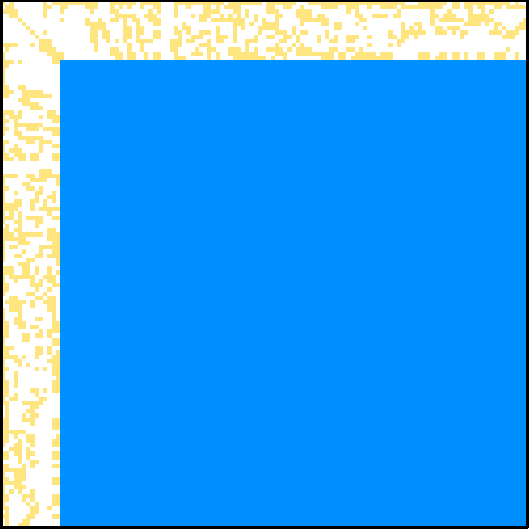
\includegraphics[width=\textwidth, keepaspectratio]{images/ch03/input-matrices/decomposition-benchmarks/msc10848_icm32pp_nan.pdf}
		\subcaption{Nonzero element pattern of the \code{LU} matrix produced by ICM\_32PP\_NaN through the decomposition of the \textit{msc10848} matrix.
The blue square indicates the presence of \code{NaN} values (\code{-NaN} in absolute value).}
		\label{Figure:comparing-decomposers-and-solvers->decomposition-project-benchmarks->decomposers-benchmark->accuracy-of-results-on-all-matrices->double-precision->matrix-with-metrics->ICM32PP-with-nan-results->msc10848->nonzero-element-pattern}
	\end{subfigure}\hspace{0.03\textwidth}
	\begin{subfigure}[t]{0.51\textwidth}
		\centering
		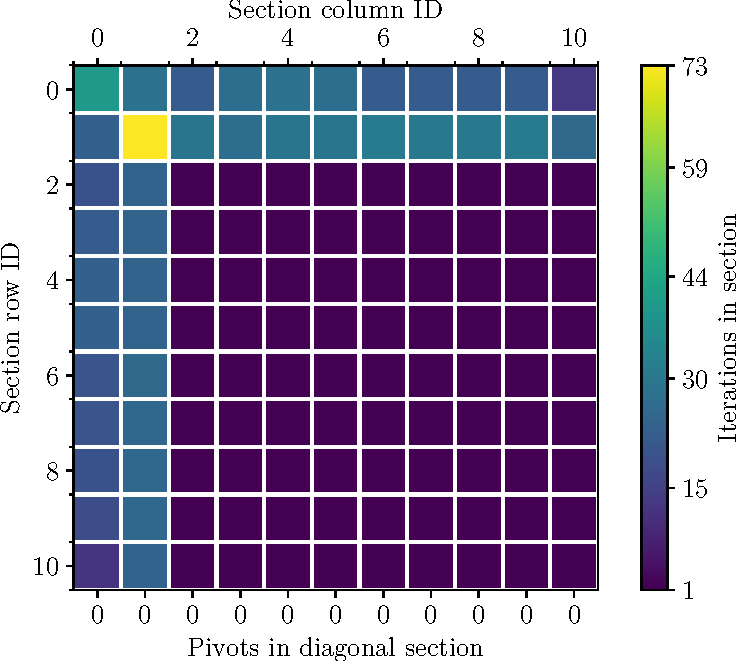
\includegraphics[width=\textwidth, keepaspectratio, clip]{images/ch03/input-matrices/decomposition-benchmarks/msc10848_icm32pp_nan_metrics.pdf}
		\subcaption{Iterative and pivoting metrics of ICM\_32PP\_NaN collected during the decomposition of the \textit{msc10848} matrix.
Each square represents a 1024-by-1024 section of the matrix.
The color in each square represents the number of iterations performed on that section.
The left and top axes show the section ID in each dimension, while the bottom axis shows the number of pivots performed in a diagonal section.}
		\label{Figure:comparing-decomposers-and-solvers->decomposition-project-benchmarks->decomposers-benchmark->accuracy-of-results-on-all-matrices->double-precision->matrix-with-metrics->ICM32PP-with-nan-results->msc10848->metrics}
	\end{subfigure}
	\caption{Nonzero element pattern of the \code{LU} matrix produced by ICM\_32PP\_NaN through the decomposition of the \textit{msc10848} matrix.
		The corresponding iterative and pivoting metrics of ICM\_32PP\_NaN are included.
	}
	\label{Figure:comparing-decomposers-and-solvers->decomposition-project-benchmarks->decomposers-benchmark->accuracy-of-results-on-all-matrices->double-precision->matrix-with-metrics->ICM32PP-with-nan-results->msc10848}
\end{figure}

As depicted in Figure~\ref{Figure:comparing-decomposers-and-solvers->decomposition-project-benchmarks->decomposers-benchmark->accuracy-of-results-on-all-matrices->double-precision->matrix-with-metrics->ICM32PP-with-nan-results->msc10848->nonzero-element-pattern}, the resulting matrix consisted mostly of \code{-NaN} values.
When considering the metrics presented in Figure~\ref{Figure:comparing-decomposers-and-solvers->decomposition-project-benchmarks->decomposers-benchmark->accuracy-of-results-on-all-matrices->double-precision->matrix-with-metrics->ICM32PP-with-nan-results->msc10848->metrics}, it can be seen that ICM\_32PP\_NaN erroneously classified the sections containing \code{-NaN} values as processed.

This issue was discovered while plotting the nonzero element patterns of the \code{LU} matrices produced by ICM\_32PP\_NaN.
The unit tests and benchmark results did not reveal any indications of invalid values.
The maximum absolute difference was calculated as follows: \code{TNL::max( TNL::abs( A - A\_res ) )}, where \code{A\_res} represents the result of \code{L*U}.
The value of the maximum absolute difference did not indicate the presence of \code{-NaN} values, as the \code{TNL::abs()} function returned \code{-NaN}.

Furthermore, as depicted in Figure~\ref{Figure:comparing-decomposers-and-solvers->decomposition-project-benchmarks->decomposers-benchmark->accuracy-of-results-on-all-matrices->double-precision->matrix-with-metrics->ICM32PP-with-nan-results->msc10848->metrics}, the dark blue sections were processed in a single iteration.
This implies that during the processing check, as shown on
Page~\pageref{Listing:implementation->decomposition-project->implemented-solutions->decomposers->ICMxPP->kernels->diagonal-compute} in Listing~\ref{Listing:implementation->decomposition-project->implemented-solutions->decomposers->ICMxPP->kernels->diagonal-compute} on Line~\ref{Line:implementation->decomposition-project->implemented-solutions->decomposers->ICMxPP->kernels->diagonal-compute->processing-check}, the \code{-NaN} values were incorrectly evaluated as processed.
Specifically, the condition \code{( abs( val - NaN ) > process\_tol )} was evaluated as \code{false} due to the \code{abs()} function also returning \code{-NaN}.

Nevertheless, how ICM\_\textit{x}PP\_NaN computed the \code{-NaN} values remains unclear.
However, it was observed that the introduction of the upper bound for conditional partial pivoting resolved the issue in all affected matrices.
Although the inclusion of the upper bound had a negative impact on the performance of ICM\_\textit{x}PP on those particular matrices, it did not affect the performance of the decomposer on the remaining matrices.
It is hypothesized that the use of the upper bound for conditional partial pivoting serves as a temporary checkpoint in the computation, effectively eliminating any potential issues that could result in the computation of \code{-NaN} values.
However, it is also possible that the introduction of the upper bound inadvertently masks another underlying issue in the implementation.

While the issue seems to have been resolved by introducing the upper bound for conditional partial pivoting, further investigation should be conducted to gain a better understanding of the underlying causes.
Additionally, to prevent similar issues from going unnoticed in the future, the result verification process for the Decomposition benchmark for decomposers ought to be revised.
The discovery of this issue revealed that the maximum absolute difference is not a reliable measure of accuracy, as it does not consider the relative accuracy of results.
For example, a maximum absolute difference of \num{1e-4} may appear reasonable, however, if the values in the input matrix are small, such as \num{1e-8}, then the resulting decomposition is highly inaccurate.

\paragraph{Single Precision} The statistical indices of the accuracy of the results obtained using single precision are presented in Table~\ref{Table:comparing-decomposers-and-solvers->decomposition-project-benchmarks->decomposers-benchmark->accuracy-of-results-on-all-matrices->single-precision->statistical-indices}.

\begin{table}[ht!]
	\centering
	\begin{tabular}{|l|r|r|r|r|r|r|}
		\hline
		\rowcolor[HTML]{C0C0C0} \multicolumn{1}{|c|}{\textbf{Decomposer}} & \multicolumn{1}{c|}{\textbf{Mean}} & \multicolumn{1}{c|}{\textbf{Std. dev.}} & \multicolumn{1}{c|}{\textbf{Q1}} & \multicolumn{1}{c|}{\textbf{Q2}} & \multicolumn{1}{c|}{\textbf{Q3}} & \multicolumn{1}{c|}{\textbf{Max.}} \\ \hline
		CMPP               & \num{6.35e+3} & \num{3.73e+4} & \num{6.10e-5} &  1.717 &  64.000 & \num{2.62e+5} \\
		CuSolverDnXgetrfPP & \num{7.49e+2} & \num{4.66e+3} & \num{9.01e-5} &  0.016 &   0.227 & \num{3.28e+4} \\
		ICM\_\textit{x}PP  & \num{6.37e+4} & \num{3.29e+5} & \num{2.08e-3} & 15.671 & 299.311 & \num{2.10e+6} \\
		PCM\_\textit{x}PP  & \num{4.96e+5} & \num{2.67e+6} &         0.002 & 27.828 & 565.789 & \num{1.84e+7} \\ \hline
	\end{tabular}
	\caption{Statistical indices of the accuracy of the results produced by the decomposers in this benchmark using single precision.
		Columns Q1, Q2, and Q3 represent the first, second, and third quartiles, respectively.
		The indices were computed using LibreOffice Calc, a spreadsheet software.
	}
	\label{Table:comparing-decomposers-and-solvers->decomposition-project-benchmarks->decomposers-benchmark->accuracy-of-results-on-all-matrices->single-precision->statistical-indices}
\end{table}

Overall, the decomposers were less accurate when using single precision.
From Table~\ref{Table:comparing-decomposers-and-solvers->decomposition-project-benchmarks->decomposers-benchmark->accuracy-of-results-on-all-matrices->single-precision->statistical-indices}, it can be seen that the mean maximum absolute difference was higher for the majority of decomposers compared to when double precision was used.
However, the values of the first and third quartiles suggest that the mean values are heavily influenced by 12 to 13 of the 50 matrices.

When using single precision, the most accurate results were produced by the CuSolverDnXgetrfPP decomposer.
Conversely, the remaining decomposers produced relatively highly inaccurate results.
Excluding CuSolverDnXgetrfPP, the most accurate decomposer was CMPP.
However, similar to double precision, the accuracy of the results produced by CMPP suffered due to conditional partial pivoting.
The accuracy of the decomposer was higher when full partial pivoting was used.
The comparison of the accuracy of results between CMPP and PCM\_\textit{x}PP, considering both conditional partial pivoting and full partial pivoting, is presented in Figure~\ref{Figure:comparing-decomposers-and-solvers->decomposition-project-benchmarks->decomposers-benchmark->accuracy-of-results-on-all-matrices->single-precision->cmpp-pcmpp-conditional-vs-full-partial-pivoting}.

\begin{figure}[ht!]
	\centering
	\tikzset{mark options={mark size=2.0, line width=0.5pt},font=\small}
	\begin{tikzpicture}
		\pgfplotstableread[col sep=comma]{resources/ch03/decomposition-benchmarks/decomposers/50-pivoting-matrices-single-precision.csv}\datatableConditionalPP
		\pgfplotstableread[col sep=comma]{resources/ch03/decomposition-benchmarks/decomposers/cmpp_pcmpp_pivot_every_element/50-pivoting-matrices-single-precision-cmpp-pcmpp-pivot-every-element.csv}\datatableFullPP
		\begin{axis}
			[
			,width=0.98\textwidth % Slightly slimmer than \textwidth to avoid warning in console for overfull \hbox
			,height=0.45\textwidth
			,axis x line*=bottom
			,axis y line*=left
			,xlabel=\textbf{Matrix ID}
			,x label style={at={(axis description cs:0.46,-.1)}}
			,ylabel=\textbf{Max. abs. difference} ($ \log $ scale)
			,xmin=-1, xmax=50
			,ymode=log
			,ymajorgrids
			,legend style={
				at={(0.5,1.025)},
				anchor=south,
				legend columns=2,
				/tikz/every even column/.append style={column sep=0.5cm},
				draw=black, % Remove legend border
				nodes={inner sep=3pt}, % Adjust the spacing between legend entries
				font=\small % Adjust the font size of the legend entries
			}
			]
			\addplot[teal,mark=triangle*] table [x=id, y=CMPP-maxAbsDiff] {\datatableConditionalPP};
			\addlegendentry{CMPP conditionalPP}
			\addplot[nvidia,mark=triangle*] table [x=id, y=PCM_8PP-maxAbsDiff] {\datatableConditionalPP};
			\addlegendentry{PCM\_\textit{x}PP conditionalPP}
			\addplot[red,mark=triangle*] table [x=id, y=CMPP-all-maxAbsDiff] {\datatableFullPP};
			\addlegendentry{CMPP fullPP}
			\addplot[cyan,mark=triangle*] table [x=id, y=PCM_8PP-all-maxAbsDiff] {\datatableFullPP};
			\addlegendentry{PCM\_\textit{x}PP fullPP}
		\end{axis}
	\end{tikzpicture}	
	\caption{Accuracy of results achieved by CMPP and PCM\_\textit{x}PP with different types of partial pivoting on the entire set of 50 matrices using single precision.
		The naming pattern for each decomposer is \textit{decomposer <type\_of\_pivoting>}.
		The vertical axis is log-scaled for better visibility.
		Note that the accuracy values for the first matrix are excluded from the plot as the results produced by the decomposers matched the expected results.
	}
	\label{Figure:comparing-decomposers-and-solvers->decomposition-project-benchmarks->decomposers-benchmark->accuracy-of-results-on-all-matrices->single-precision->cmpp-pcmpp-conditional-vs-full-partial-pivoting}
\end{figure}

Figure~\ref{Figure:comparing-decomposers-and-solvers->decomposition-project-benchmarks->decomposers-benchmark->accuracy-of-results-on-all-matrices->single-precision->cmpp-pcmpp-conditional-vs-full-partial-pivoting} highlights the instability of conditional partial pivoting.
Specifically, it demonstrates that the difference in accuracy between CMPP conditionalPP and PCM\_xPP conditionalPP is much greater with single precision compared to double precision.
These results indicate that conditional partial pivoting, when combined with lower precision, leads to an unstable approach that produces inaccurate results.

To summarize the accuracy of results on all matrices, the decomposer that consistently produced the most accurate results regardless of the precision used was CuSolverDnXgetrfPP.
Excluding CuSolverDnXgetrfPP, CMPP is recommended for both double and single precision in terms of accuracy.
However, if high accuracy is required, then CMPP with full partial pivoting is more suitable compared to CMPP with conditional partial pivoting.

\paragraph{Summary of Decomposers Benchmark} The fastest and most accurate decomposer on the set of 50 matrices was CuSolverDnXgetrfPP.
Among the decomposers implemented by the author of this thesis, PCM\_8PP is a suitable choice if execution speed is the primary requirement, as it consistently performs well.
However, for sparse matrices with most of their elements on the main diagonal, ICM\_32PP can be a suitable alternative.
Furthermore, for specific problems, such as the "Poisson equation on a cube" problem implemented in BDDCML, ICM\_32PP may outperform PCM\_8PP.
On the other hand, if highly accurate results are required, CMPP is recommended, even at the cost of execution speed.



\subsection{Solvers Benchmark}\label{Subsection:comparing-decomposers-and-solvers->decomposition-project-benchmarks->solvers-benchmark}
This section presents benchmark results obtained by solving systems of linear equations that originated from the set of 50 matrices.
The benchmark for solvers consists of each matrix being used as a coefficient matrix $\mathbf{A}$ in $\mathbf{AX} = \mathbf{B}$.
Specifically, the benchmark comprises the following steps:

\begin{tight_enumerate}
	\item The matrix is decomposed either by CMPP or GEM depending on which of the two matrices, \code{L} or \code{U}, is expected by the solver to contain a unit diagonal.
If the unit diagonal is expected in \code{U}, then CMPP is used, whereas if it is expected in \code{L}, then GEM is used.
	\item To mitigate possible inaccuracies caused by the decomposer, matrices \code{L} and \code{U} are multiplied to create \code{A\_res} which is later used instead of \code{A} for the verification of results.
	\item The matrix of 10 right-hand sides, \code{B}, is filled with ones.
	\item The solver receives the decomposed matrices, \code{L} and \code{U}, the pivoting vector \code{piv}, the matrix of unknowns, \code{X}, and the matrix of right-hand sides, \code{B}.
	\item The system is solved 10 times by the solver, and the collected metrics are subsequently averaged and logged.
\end{tight_enumerate}

The solvers compared in this benchmark are listed in Table~\ref{Table:comparing-decomposers-and-solvers->decomposition-project-benchmarks->solvers-benchmark->table-of-solvers}.

\begin{table}[ht!]
	\centering
	\begin{tabular}{|ll|c|c|}
		\hline
		\rowcolor[HTML]{C0C0C0} 
		\multicolumn{2}{|c|}{\cellcolor[HTML]{C0C0C0}\textbf{Solver}} & \cellcolor[HTML]{C0C0C0} & \multicolumn{1}{c|}{\cellcolor[HTML]{C0C0C0}} \\
		\rowcolor[HTML]{EFEFEF} 
		\multicolumn{1}{|c|}{\cellcolor[HTML]{EFEFEF}\textbf{Name}} & \multicolumn{1}{c|}{\cellcolor[HTML]{EFEFEF}\textbf{Abbreviation}} & \multirow{-2}{*}{\cellcolor[HTML]{C0C0C0}\textbf{Variants}} & \multicolumn{1}{c|}{\multirow{-2}{*}{\cellcolor[HTML]{C0C0C0}\textbf{Performer}}} \\ \hline
		\multicolumn{1}{|l|}{Sequential Solver with Partial Piv.} & SSPP               &         -          & CPU \\
		\multicolumn{1}{|l|}{CuBLAStrsm with Partial Piv.}        & CuBLAStrsmPP       &         -          & GPU \\
		\multicolumn{1}{|l|}{CuSolverDnXgetrs with Partial Piv.}  & CuSolverDnXgetrsPP &         -          & GPU \\
		\multicolumn{1}{|l|}{Iterative Solver with Partial Piv.}  & IS\_\textit{x}PP   & 8, 16, 32, 64, 128 & GPU \\ \hline
	\end{tabular}
	\caption{Solvers compared in the benchmark: SSPP (described in \namerefItalics{Paragraph:implementation->decomposition-project->implemented-solutions->solvers->SSPP} in Section~\ref{Subsection:implementation->decomposition-project->implemented-solutions->solvers}), CuBLAStrsmPP (mentioned in Section~\ref{Subsection:implementation->libraries-used->CUDA-libraries->cuBLAS}), CuSolverDnXgetrsPP (mentioned in Section~\ref{Subsection:implementation->libraries-used->CUDA-libraries->cuSOLVER}), and IS\_\textit{x}PP (described in \namerefItalics{Paragraph:implementation->decomposition-project->implemented-solutions->solvers->ISxPP} in Section~\ref{Subsection:implementation->decomposition-project->implemented-solutions->solvers}).
		The \textit{Variants} column indicates the different configurations of each solver.
		The IS\_\textit{x}PP solver was benchmarked as five separate solvers depending on the CUDA thread block configuration.
		The \textit{x} in IS\_\textit{x}PP represents the number of threads per block in the 1st dimension.
		The \textit{Performer} column specifies the primary device used by each solver.
		The CuBLAStrsmPP solver assumed that the unit diagonal was present in matrix \code{U}.
	}
	\label{Table:comparing-decomposers-and-solvers->decomposition-project-benchmarks->solvers-benchmark->table-of-solvers}
\end{table}

Note that the processing tolerance of IS\_\textit{x}PP was set to zero, as higher accuracy of the produced results is required.
As mentioned in Section~\ref{Subsection:implementation->decomposition-project->implemented-solutions->solvers}, the implementation of solvers was not part of the diploma thesis assignment.
Furthermore, neither SSPP nor IS\_\textit{x}PP were prioritized in terms of optimization.
Therefore, the benchmark results of the solvers will only be presented briefly for the entire set of 50 matrices.

First, the execution times of the solvers listed in Table~\ref{Table:comparing-decomposers-and-solvers->decomposition-project-benchmarks->solvers-benchmark->table-of-solvers} on the set of 50 matrices are presented for both double and single precision.
Then, the accuracy of the results is discussed.


\subsubsection{Comparison of Execution Times on All Matrices}
The comparison of execution times of the solvers listed in Table~\ref{Table:comparing-decomposers-and-solvers->decomposition-project-benchmarks->solvers-benchmark->table-of-solvers} on the set of 50 matrices using both double and single precision is presented in Figure~\ref{Figure:comparing-decomposers-and-solvers->decomposition-project-benchmarks->solvers-benchmark->comparison-of-execution-times-on-all-matrices->double-and-single-precision}.

\begin{figure}[ht!]
	\centering
	\tikzset{mark options={mark size=1.5},font=\small}
	\begin{subfigure}{\textwidth}
		\begin{tikzpicture}
			\pgfplotstableread[col sep=comma]{resources/ch03/decomposition-benchmarks/solvers/50-pivoting-matrices-double-precision.csv}\datatable
			\begin{axis}
				[
				,width=0.975\textwidth % Slightly slimmer than \textwidth to avoid warning in console for overfull \hbox
				,height=0.45\textwidth
				,axis x line*=bottom
				,axis y line*=left
				,xlabel=\textbf{Matrix ID}
				,ylabel={\textbf{Execution time [s]} ($\log$ scale)}
				,x label style={at={(axis description cs:0.46,-.1)}}
				,xmin=-1, xmax=50
				,ymode=log
				,ymajorgrids
				,legend style={
					at={(0.5,1.025)},
					anchor=south,
					legend columns=4,
					/tikz/every even column/.append style={column sep=0.5cm},
					draw=black, % Remove legend border
					nodes={inner sep=3pt}, % Adjust the spacing between legend entries
					font=\small % Adjust the font size of the legend entries
				}
				]
				\addplot[red,mark=triangle*] table [x=id, y=CuBLAStrsmPP-time] {\datatable};
				\addlegendentry{CuBLAStrsmPP}
				\addplot[black,mark=triangle*] table [x=id, y=SSPP-time] {\datatable};
				\addlegendentry{SSPP}
				\addplot[blue,mark=triangle*] table [x=id, y=IS_8PP-time] {\datatable};
				\addlegendentry{IS\_8PP}
				\addplot[purple,mark=triangle*] table [x=id, y=IS_16PP-time] {\datatable};
				\addlegendentry{IS\_16PP}
				\addplot[teal,mark=triangle*] table [x=id, y=IS_32PP-time] {\datatable};
				\addlegendentry{IS\_32PP}
				\addplot[green!60!black,mark=triangle*] table [x=id, y=CuSolverDnXgetrsPP-time] {\datatable};
				\addlegendentry{CuSolverDnXgetrsPP}
				\addplot[nvidia,mark=triangle*] table [x=id, y=IS_64PP-time] {\datatable};
				\addlegendentry{IS\_64PP}
				\addplot[cyan,mark=triangle*] table [x=id, y=IS_128PP-time] {\datatable};
				\addlegendentry{IS\_128PP}
			\end{axis}
		\end{tikzpicture}
		\subcaption{Double precision}
		\label{Figure:comparing-decomposers-and-solvers->decomposition-project-benchmarks->solvers-benchmark->comparison-of-execution-times-on-all-matrices->double-precision}
	\end{subfigure}
	\begin{subfigure}{\textwidth}
		\begin{tikzpicture}
			\pgfplotstableread[col sep=comma]{resources/ch03/decomposition-benchmarks/solvers/50-pivoting-matrices-single-precision.csv}\datatable
			\begin{axis}
				[
				,width=0.975\textwidth % Slightly slimmer than \textwidth to avoid warning in console for overfull \hbox
				,height=0.45\textwidth
				,axis x line*=bottom
				,axis y line*=left
				,xlabel=\textbf{Matrix ID}
				,ylabel={\textbf{Execution time [s]} ($\log$ scale)}
				,x label style={at={(axis description cs:0.46,-.1)}}
				,xmin=-1, xmax=50
				,ymode=log
				,ymajorgrids
				]
				\addplot[red,mark=triangle*] table [x=id, y=CuBLAStrsmPP-time] {\datatable};
				\addplot[black,mark=triangle*] table [x=id, y=SSPP-time] {\datatable};
				\addplot[blue,mark=triangle*] table [x=id, y=IS_8PP-time] {\datatable};
				\addplot[purple,mark=triangle*] table [x=id, y=IS_16PP-time] {\datatable};
				\addplot[teal,mark=triangle*] table [x=id, y=IS_32PP-time] {\datatable};
				\addplot[green!60!black,mark=triangle*] table [x=id, y=CuSolverDnXgetrsPP-time] {\datatable};
				\addplot[nvidia,mark=triangle*] table [x=id, y=IS_64PP-time] {\datatable};
				\addplot[cyan,mark=triangle*] table [x=id, y=IS_128PP-time] {\datatable};
			\end{axis}
		\end{tikzpicture}
		\subcaption{Single precision}
		\label{Figure:comparing-decomposers-and-solvers->decomposition-project-benchmarks->solvers-benchmark->comparison-of-execution-times-on-all-matrices->single-precision}
	\end{subfigure}
	\caption{Execution times (in seconds) of solvers listed in Table~\ref{Table:comparing-decomposers-and-solvers->decomposition-project-benchmarks->solvers-benchmark->table-of-solvers} on the set of 50 matrices using double and single precision.
		The vertical axis is log-scaled for improved visibility.
	}
	\label{Figure:comparing-decomposers-and-solvers->decomposition-project-benchmarks->solvers-benchmark->comparison-of-execution-times-on-all-matrices->double-and-single-precision}
\end{figure}

As depicted in Figure~\ref{Figure:comparing-decomposers-and-solvers->decomposition-project-benchmarks->solvers-benchmark->comparison-of-execution-times-on-all-matrices->double-and-single-precision}, CuBLAStrsmPP and CuSolverDnXgetrsPP were the fastest solvers overall, regardless of the precision used.
The results indicate that, similar to ICM\_\textit{x}PP, the performance of the iterative approach of IS\_\textit{x}PP depends on the characteristics of the matrix.
For example, when double precision was used, IS\_\textit{x}PP outperformed SSPP on 26 out of the 50 matrices.
These 26 matrices were made up of 19 sparse matrices from \citetitle{Davis2011} \cite{Davis2011} and seven dense matrices from the "Poisson equation on cube" problem implemented in BDDCML.
When considering matrices with dimensions up to approximately 3600-by-3600 (matrices 0 to 29), it can be seen that the execution times of IS\_\textit{x}PP are closer to those of the established CUDA solvers compared to matrices with larger dimensions.
This suggests that the performance of IS\_\textit{x}PP and SSPP does not scale well.

Additionally, when examining the variants of IS\_\textit{x}PP, it is evident that IS\_128PP is consistently surpassed by variants with a smaller number of threads per block, for both double and single precision.
To confirm this observation, Figure~\ref{Figure:comparing-decomposers-and-solvers->decomposition-project-benchmarks->solvers-benchmark->comparison-of-execution-times-on-all-matrices->ISxPP-double-precision} presents a comparison of execution times for the IS\_\textit{x}PP variants on the set of matrices when double precision was used.

\begin{figure}[ht!]
	\centering
	\tikzset{mark options={mark size=2.0, line width=0.5pt},font=\small}
	\begin{tikzpicture}
		\pgfplotstableread[col sep=comma]{resources/ch03/decomposition-benchmarks/solvers/50-pivoting-matrices-double-precision.csv}\datatable
		\begin{axis}
			[
			,width=0.98\textwidth
			,height=0.45\textwidth
			,axis x line*=bottom
			,axis y line*=left
			,xlabel=\textbf{Matrix ID}
			,ylabel={\textbf{Execution time [s]} ($\log$ scale)}
			,x label style={at={(axis description cs:0.46,-.1)}}
			,xmin=-1, xmax=50
			,ymode=log
			,ymajorgrids
			,legend style={
				at={(0.5,1.025)},
				anchor=south,
				legend columns=5,
				/tikz/every even column/.append style={column sep=0.5cm},
				draw=black, % Remove legend border
				nodes={inner sep=3pt}, % Adjust the spacing between legend entries
				font=\small % Adjust the font size of the legend entries
			}
			]
			\addplot[blue,mark=triangle*] table [x=id, y=IS_8PP-time] {\datatable};
			\addlegendentry{IS\_8PP}
			\addplot[purple,mark=triangle*] table [x=id, y=IS_16PP-time] {\datatable};
			\addlegendentry{IS\_16PP}
			\addplot[teal,mark=triangle*] table [x=id, y=IS_32PP-time] {\datatable};
			\addlegendentry{IS\_32PP}
			\addplot[nvidia,mark=triangle*] table [x=id, y=IS_64PP-time] {\datatable};
			\addlegendentry{IS\_64PP}
			\addplot[cyan,mark=triangle*] table [x=id, y=IS_128PP-time] {\datatable};
			\addlegendentry{IS\_128PP}
		\end{axis}
	\end{tikzpicture}	
	\caption{Execution times (in seconds) of the variants of IS\_\textit{x}PP on the set of 50 matrices using double precision.
		The vertical axis is log-scaled for improved visibility.
	}
	\label{Figure:comparing-decomposers-and-solvers->decomposition-project-benchmarks->solvers-benchmark->comparison-of-execution-times-on-all-matrices->ISxPP-double-precision}
\end{figure}

As depicted in Figure~\ref{Figure:comparing-decomposers-and-solvers->decomposition-project-benchmarks->solvers-benchmark->comparison-of-execution-times-on-all-matrices->ISxPP-double-precision}, IS\_8PP consistently demonstrated better performance compared to IS\_16PP, which in turn consistently outperformed IS\_32P, and so on.
These findings suggest that IS\_\textit{x}PP is also affected by the resource idleness issue described on Page~\pageref{Paragraph:comparing-decomposers-and-solvers->decomposition-project-benchmarks->decomposers-benchmark->comparison-of-execution-times-on-subset-of-matrices->PCMxPP} for PCM\_\textit{x}PP.
In IS\_\textit{x}PP, the thread blocks comprise \textit{x}-by-8 threads, as shown in Listing~\ref{Listing:ISxPP-implementation-excerpt} on Line~\ref{Line:ISxPP-implementation-excerpt->num-threads-per-block}.
Each row of threads within the eight rows of threads in the thread block is responsible for computing values for one right-hand side.
The number of rows in the thread block has remained constant since the initial implementation of the solver.
As solvers were not a part of the diploma thesis assignment, the implementation of thread blocks that would dynamically adapt to the number of right-hand sides was not prioritized.
Each thread in the 1st dimension is responsible for computing one element of a right-hand side.
For example, thread \code{(x = 10, y = 5)} is responsible for computing the 10th element of the 5th right-hand side.

To aid the explanation of the resource idleness that arises in IS\_\textit{x}PP as a result of its thread block structure, the visualizations of forward and backward substitution are shown in Figure~\ref{Figure:comparing-decomposers-and-solvers->decomposition-project-benchmarks->solvers-benchmark->comparison-of-execution-times-on-all-matrices->visualization-of-substitutions}.

\begin{figure}[ht!]
	\centering
	\begin{subfigure}[b]{0.48\textwidth}
		\centering
		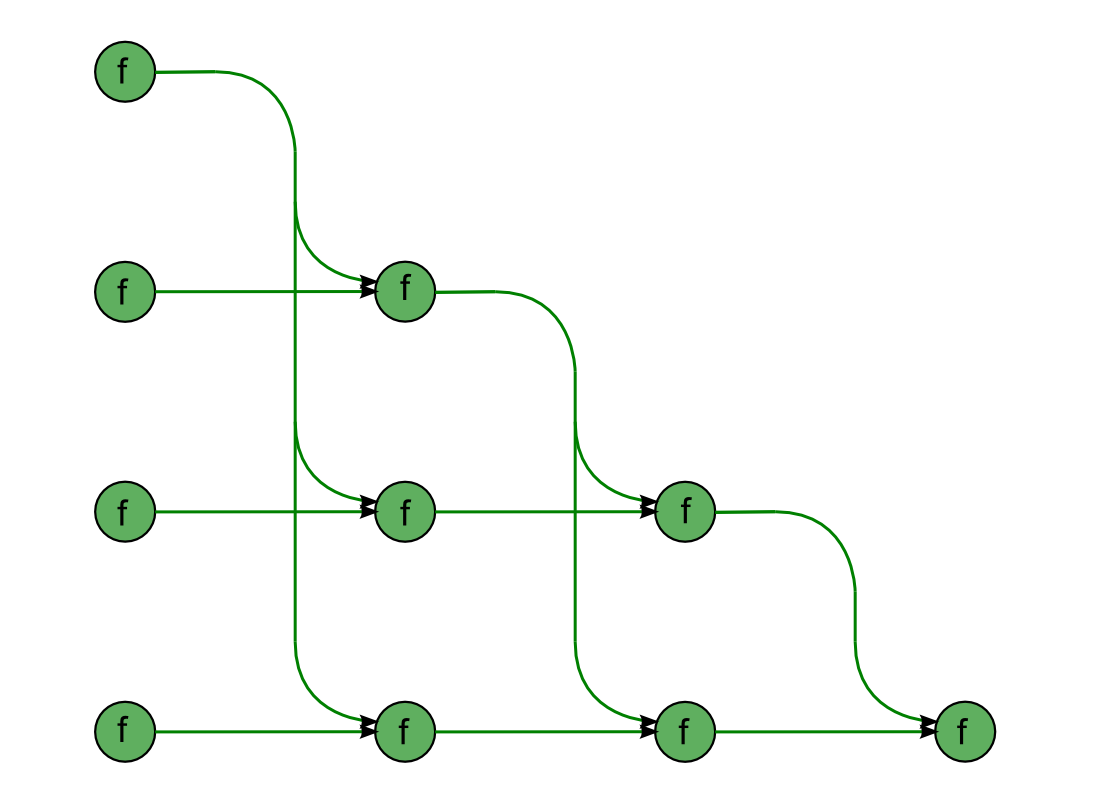
\includegraphics[width=\textwidth]{images/ch03/procedures/forward-substitution.png}
		\caption{Forward substitution}
		\label{Figure:comparing-decomposers-and-solvers->decomposition-project-benchmarks->solvers-benchmark->comparison-of-execution-times-on-all-matrices->visualization-of-substitutions->forward}
	\end{subfigure}\hspace{0.03\textwidth}
	\begin{subfigure}[b]{0.48\textwidth}
		\centering
		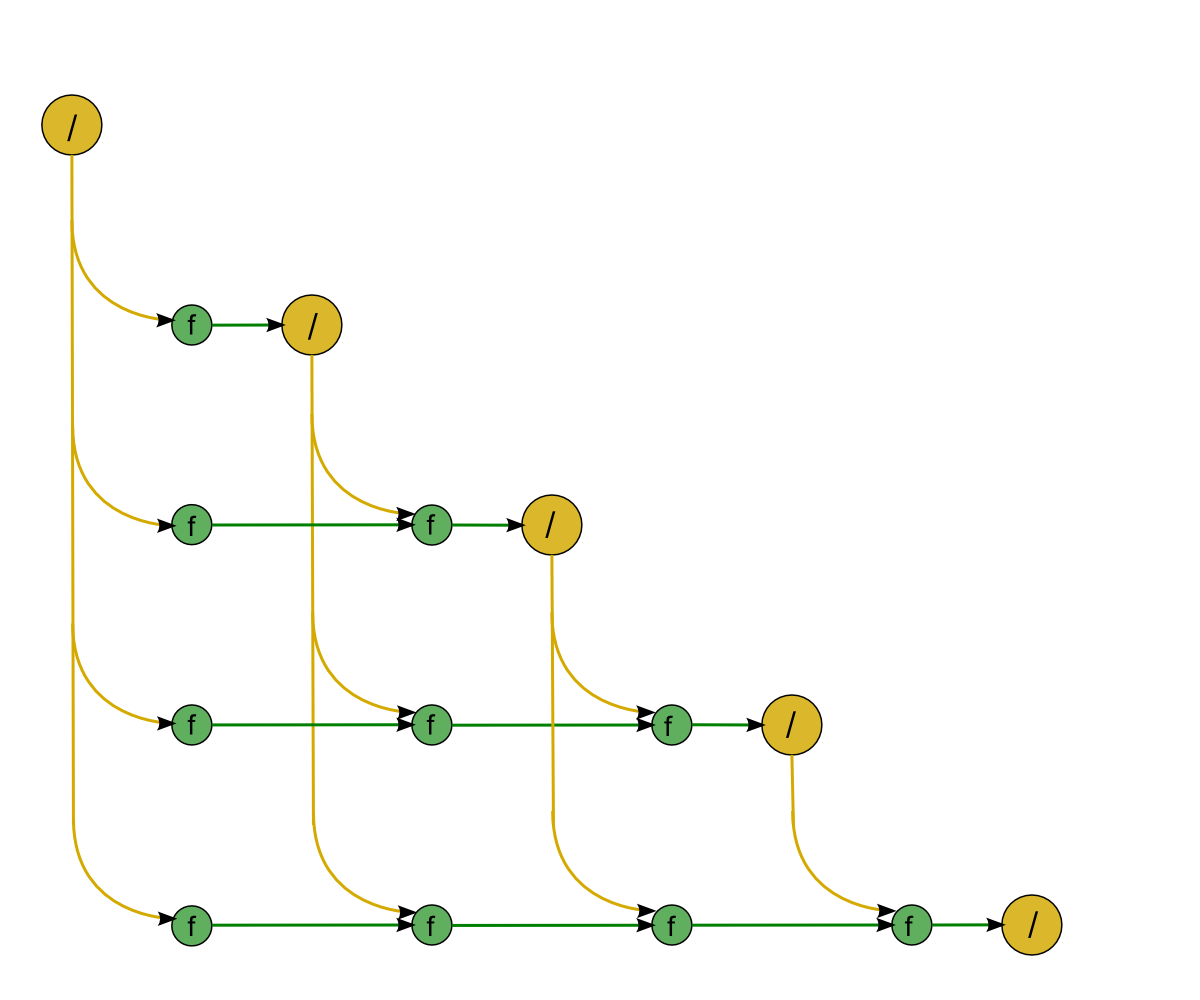
\includegraphics[width=\textwidth]{images/ch03/procedures/backward-substitution.png}
		\caption{Backward substitution}
		\label{Figure:comparing-decomposers-and-solvers->decomposition-project-benchmarks->solvers-benchmark->comparison-of-execution-times-on-all-matrices->visualization-of-substitutions->backward}
	\end{subfigure}
	\caption{Visualizations of the forward and backward substitution algorithms.
		The visualizations assume a single right-hand side.
		Each row in both figures represents the computation of one value in the output vector of the substitution.
		The arrows indicate the use of previously-computed values in the computation of succeeding values.
		Taken from \citetitle{Frolov18July2022} \cite{Frolov18July2022} and \citetitle{Frolov17July2022} \cite{Frolov17July2022}.
	}
	\label{Figure:comparing-decomposers-and-solvers->decomposition-project-benchmarks->solvers-benchmark->comparison-of-execution-times-on-all-matrices->visualization-of-substitutions}
\end{figure}

For simplicity, hereafter, the substitutions are assumed to work with only one right-hand side, unless stated otherwise.
In Figures~\ref{Figure:comparing-decomposers-and-solvers->decomposition-project-benchmarks->solvers-benchmark->comparison-of-execution-times-on-all-matrices->visualization-of-substitutions->forward} and \ref{Figure:comparing-decomposers-and-solvers->decomposition-project-benchmarks->solvers-benchmark->comparison-of-execution-times-on-all-matrices->visualization-of-substitutions->backward}, each row represents the computation of a value by its assigned thread.
Since a warp comprises 32 threads, each warp is responsible for computing 32 adjacent elements.
Starting with the first thread of the warp, each subsequent thread performs an additional calculation.
For example, thread \code{0} computes the value with one calculation, while thread \code{1} computes the value with two calculations, and so on.
Therefore, the time it takes for each warp to complete its work depends on the thread with the most calculations to perform, i.e., the last thread.

The number of threads per block for IS\_8PP, IS\_16PP, IS\_32PP, IS\_64PP, and IS\_128PP is 64, 128, 256, 512, and 1024, respectively.
The maximum number of thread blocks per SM for each variant is 32, 16, 8, 4, and 2, respectively.
For example, IS\_128PP can only allocate two thread blocks per SM.
Since each thread block covers the computation of 128 elements, the thread computing the last element has to perform an additional 128 calculations compared to the first thread of the block.
Therefore, while the threads of the last warp are still computing their elements, the warps preceding the last warp are idle as they will have completed their work earlier.
In other words, the last warp of each thread block holds the thread block in an SM, preventing the scheduling of another thread block.

As with PCM\_\textit{x}PP, the variants of IS\_\textit{x}PP with fewer threads per block were able to utilize SMs more efficiently, as more of their smaller blocks could be allocated per SM.
It can be argued that the idleness of resources is further exacerbated by the fixed size of the 2nd dimension of the thread block, which is set to eight.
If the number of threads per block were to adapt to the number of right-hand sides, the number of threads in each block would decrease, enabling the allocation of more blocks per SM.

To put the results into perspective, Table~\ref{Table:comparing-decomposers-and-solvers->decomposition-project-benchmarks->solvers-benchmark->comparison-of-execution-times-on-all-matrices->total-execution-time-of-solvers-on-set-of-50-matrices} displays the total time taken by each solver to solve systems derived from the entire set of 50 matrices.

\begin{table}[ht!]
	\centering
	\begin{tabular}{|l|r|r|}
		\hline
		\rowcolor[HTML]{C0C0C0} 
		\multicolumn{1}{|c|}{\cellcolor[HTML]{C0C0C0}}                                      & \multicolumn{2}{c|}{\cellcolor[HTML]{C0C0C0}\textbf{Total execution time {[}s{]}}}                                                                        \\ \cline{2-3} 
		\rowcolor[HTML]{EFEFEF} 
		\multicolumn{1}{|c|}{\multirow{-2}{*}{\cellcolor[HTML]{C0C0C0}\textbf{Solver}}} & \multicolumn{1}{l|}{\cellcolor[HTML]{EFEFEF}\textbf{Double precision}} & \multicolumn{1}{l|}{\cellcolor[HTML]{EFEFEF}\textbf{Single Precision}} \\ \hline
		\multicolumn{1}{|l|}{SSPP}               & 120.963 & 114.645 \\
		\multicolumn{1}{|l|}{CuBLAStrsmPP}       &   0.479 &   0.209 \\
		\multicolumn{1}{|l|}{CuSolverDnXgetrsPP} &   0.505 &   0.274 \\
		\multicolumn{1}{|l|}{IS\_128PP}          & 561.879 & 414.728 \\
		\multicolumn{1}{|l|}{IS\_16PP}           & 282.535 & 156.937 \\
		\multicolumn{1}{|l|}{IS\_32PP}           & 351.020 & 279.547 \\
		\multicolumn{1}{|l|}{IS\_64PP}           & 415.793 & 334.692 \\
		\multicolumn{1}{|l|}{IS\_8PP}            & 224.219 & 115.321 \\ \hline
	\end{tabular}
	\caption{Total execution time (in seconds) taken by each solver to solve systems derived from the set of 50 matrices using double and single precision.
		The execution times are rounded to three decimal places.
	}
	\label{Table:comparing-decomposers-and-solvers->decomposition-project-benchmarks->solvers-benchmark->comparison-of-execution-times-on-all-matrices->total-execution-time-of-solvers-on-set-of-50-matrices}
\end{table}

As demonstrated in Figure~\ref{Figure:comparing-decomposers-and-solvers->decomposition-project-benchmarks->solvers-benchmark->comparison-of-execution-times-on-all-matrices->double-and-single-precision} and confirmed in Table~\ref{Table:comparing-decomposers-and-solvers->decomposition-project-benchmarks->solvers-benchmark->comparison-of-execution-times-on-all-matrices->total-execution-time-of-solvers-on-set-of-50-matrices}, the fastest solver for the set of 50 matrices was CuBLAStrsmPP.
Excluding the solvers from CUDA libraries, SSPP was the fastest solver, even though it outperformed IS\_8PP on only 24 out of 50 matrices.


\subsubsection{Accuracy of Results on All Matrices}\label{Subsection:comparing-decomposers-and-solvers->decomposition-project-benchmarks->solvers-benchmark->accuracy-of-results-on-all-matrices}
The accuracy of the values of unknowns produced by solvers is a crucial performance indicator.
The maximum absolute difference between the expected results and the actual results for the set of 50 matrices using both double and single precision is presented in Figure~\ref{Figure:comparing-decomposers-and-solvers->decomposition-project-benchmarks->solvers-benchmark->accuracy-of-results-on-all-matrices->double-and-single-precision}.
For context, the maximum absolute difference for solvers was defined in Equation~\ref{Equation:implementation->decomposition-project->benchmarks->solvers->maximum-difference} as $\max \left| \mathbf{LUPX} - \mathbf{B} \right|$, where $\mathbf{L}$ (lower-triangular matrix), $\mathbf{U}$ (unit upper-triangular matrix), and $\mathbf{P}$ (permutation matrix) are the results of the decomposition operation performed on the input matrix; $\mathbf{X}$ represents the matrix of unknowns whose values are computed by a solver, and $\mathbf{B}$ denotes the matrix of right-hand sides (with all values equal to 1).
Note that the permutation matrix was represented by a vector in the implementations.
This section mentions the IS\_\textit{x}PP solver instead of its variants, as they did not differ in terms of accuracy, i.e., there was no need to specifically address each variant.

\begin{figure}[ht!]
	\centering
	\tikzset{mark options={mark size=1.5},font=\small}
	\begin{subfigure}{\textwidth}
		\begin{tikzpicture}
			\pgfplotstableread[col sep=comma]{resources/ch03/decomposition-benchmarks/solvers/50-pivoting-matrices-double-precision.csv}\datatable
			\begin{axis}
				[
				,width=0.975\textwidth % Slightly slimmer than \textwidth to avoid warning in console for overfull \hbox
				,height=0.45\textwidth
				,axis x line*=bottom
				,axis y line*=left
				,xlabel=\textbf{Matrix ID}
				,ylabel=\textbf{Max. abs. difference} ($\log$ scale)
				,x label style={at={(axis description cs:0.46,-.1)}}
				,xmin=-1, xmax=50
				,ymode=log
				,ymajorgrids
				,legend style={
					at={(0.5,1.025)},
					anchor=south,
					legend columns=4,
					/tikz/every even column/.append style={column sep=0.5cm},
					draw=black, % Remove legend border
					nodes={inner sep=3pt}, % Adjust the spacing between legend entries
					font=\small % Adjust the font size of the legend entries
				}
				]
				% Matrices for which IS_xPP computed invalid values: 23, 44, 47, 49
				% Must use \pgfplotsinvokeforeach since 'axis' is for pgfplots and foreach is for tikz? - see https://tex.stackexchange.com/a/170670/182615
				\pgfplotsinvokeforeach{23, 44, 47, 49}{
					\draw[blue,thick] ({axis cs:#1,0}|-{rel axis cs:0,0}) -- ({axis cs:#1,0}|-{rel axis cs:0,1});
				}
				
				\addplot[red,mark=triangle*] table [x=id, y=CuBLAStrsmPP-maxAbsDiff] {\datatable};
				\addlegendentry{CuBLAStrsmPP}
				\addplot[black,mark=triangle*] table [x=id, y=SSPP-maxAbsDiff] {\datatable};
				\addlegendentry{SSPP}
				\addplot[blue,mark=triangle*] table [x=id, y=IS_8PP-maxAbsDiff] {\datatable};
				\addlegendentry{IS\_\textit{x}PP}
				\addplot[green!60!black,mark=triangle*] table [x=id, y=CuSolverDnXgetrsPP-maxAbsDiff] {\datatable};
				\addlegendentry{CuSolverDnXgetrsPP}
			\end{axis}
		\end{tikzpicture}
		\subcaption{Double precision}
		\label{Figure:comparing-decomposers-and-solvers->decomposition-project-benchmarks->solvers-benchmark->accuracy-of-results-on-all-matrices->double-precision}
	\end{subfigure}
	\begin{subfigure}{\textwidth}
		\begin{tikzpicture}
			\pgfplotstableread[col sep=comma]{resources/ch03/decomposition-benchmarks/solvers/50-pivoting-matrices-single-precision.csv}\datatable
			\begin{axis}
				[
				,width=0.975\textwidth % Slightly slimmer than \textwidth to avoid warning in console for overfull \hbox
				,height=0.45\textwidth
				,axis x line*=bottom
				,axis y line*=left
				,xlabel=\textbf{Matrix ID}
				,ylabel=\textbf{Max. abs. difference} ($\log$ scale)
				,x label style={at={(axis description cs:0.46,-.1)}}
				,xmin=-1, xmax=50
				,ymode=log
				,ymajorgrids
				]
				% Matrices for which IS_xPP computed invalid values: 10, 15, 21, 23, 25, 33, 34, 35, 42, 44, 47, 49
				% Must use \pgfplotsinvokeforeach since 'axis' is for pgfplots and foreach is for tikz? - see https://tex.stackexchange.com/a/170670/182615
				\pgfplotsinvokeforeach{10, 15, 21, 23, 25, 33, 34, 35, 42, 44, 47, 49}{
					\draw[blue,thick] ({axis cs:#1,0}|-{rel axis cs:0,0}) -- ({axis cs:#1,0}|-{rel axis cs:0,1});
				}
				
				\addplot[red,mark=triangle*] table [x=id, y=CuBLAStrsmPP-maxAbsDiff] {\datatable};
				\addplot[black,mark=triangle*] table [x=id, y=SSPP-maxAbsDiff] {\datatable};
				\addplot[blue,mark=triangle*] table [x=id, y=IS_8PP-maxAbsDiff] {\datatable};
				\addplot[green!60!black,mark=triangle*] table [x=id, y=CuSolverDnXgetrsPP-maxAbsDiff] {\datatable};
			\end{axis}
		\end{tikzpicture}
		\subcaption{Single precision}
		\label{Figure:comparing-decomposers-and-solvers->decomposition-project-benchmarks->solvers-benchmark->accuracy-of-results-on-all-matrices->single-precision}
	\end{subfigure}
	\caption{Accuracy of results achieved by the solvers listed in Table~\ref{Table:comparing-decomposers-and-solvers->decomposition-project-benchmarks->solvers-benchmark->table-of-solvers} (excluding the different variants) on the entire set of 50 matrices using both double and single precision.
		The matrix ID represents the ID of the matrices after they have been sorted according to their dimensions from smallest to largest.
		The vertical axis is log-scaled for improved visibility.
		The blue vertical lines indicate matrices for which IS\_\textit{x}PP produced invalid results.
		The accuracy values for the invalid results were not plotted to avoid distorting the vertical axis and allow for comparison of the remaining accuracy values.
		Additionally, it is important to mention that the vertical axes of both graphs do not cover the same range.
	}
	\label{Figure:comparing-decomposers-and-solvers->decomposition-project-benchmarks->solvers-benchmark->accuracy-of-results-on-all-matrices->double-and-single-precision}
\end{figure}

As mentioned in the caption of Figure~\ref{Figure:comparing-decomposers-and-solvers->decomposition-project-benchmarks->solvers-benchmark->accuracy-of-results-on-all-matrices->double-and-single-precision}, IS\_\textit{x}PP occasionally produced invalid results.
Specifically, when using double precision, for four matrices, the solver produced results that resulted in the maximum absolute difference being equal to \num{1.797693e+308}, which is the highest possible value that a variable of type \code{double} can store.
In the case of single precision, the solver produced invalid results for twelve matrices, with the maximum absolute difference equal to -\num{3.402823E+038} which is close to the lowest possible value that a variable of type \code{float} can store.
Among the twelve matrices, eleven were sparse, and one was dense.
Additionally, it is worth noting that the CPU version of IS\_\textit{x}PP also produced the same invalid results, indicating that the issue lies with the algorithm itself rather than the GPU implementation.
The reason behind IS\_\textit{x}PP computing invalid values in the mentioned cases is currently unclear.
One possible hypothesis is that the computation of certain values is being skipped, leading to a cascade of erroneous calculations.

For completeness, the statistical indices of the accuracy of the results produced by the solvers are presented in Table~\ref{Table:comparing-decomposers-and-solvers->decomposition-project-benchmarks->solvers-benchmark->accuracy-of-results-on-all-matrices->statistical-indices->double-precision} for double precision and in Table~\ref{Table:comparing-decomposers-and-solvers->decomposition-project-benchmarks->solvers-benchmark->accuracy-of-results-on-all-matrices->statistical-indices->single-precision} for single precision.
Note that both tables contain two instances of IS\_\textit{x}PP: IS\_\textit{x}PP and IS\_\textit{x}PP\_inv.
The former does not consider the invalid values in its indices, while the latter does.

\begin{table}[ht!]
	\centering
	\begin{tabular}{|l|r|r|r|r|r|r|}
		\hline
		\rowcolor[HTML]{C0C0C0} \multicolumn{1}{|c|}{\textbf{Solver}} & \multicolumn{1}{c|}{\textbf{Mean}} & \multicolumn{1}{c|}{\textbf{Std. dev.}} & \multicolumn{1}{c|}{\textbf{Q1}} & \multicolumn{1}{c|}{\textbf{Q2}} & \multicolumn{1}{c|}{\textbf{Q3}} & \multicolumn{1}{c|}{\textbf{Max.}} \\ \hline
		SSPP                  &   \num{4.20e+4} &   \num{2.97e+5} & \num{5.82e-11} &  \num{4.38e-8} &  \num{4.99e-6} &   \num{2.10e+6} \\
		CBLAStrsmPP           &   \num{4.20E+4} &   \num{2.97e+5} & \num{4.08e-11} &  \num{8.75e-8} &  \num{6.70e-6} &   \num{2.10e+6} \\
		CSDnXgetsfPP          &   \num{4.19e+4} &   \num{2.97e+5} & \num{1.96e-12} & \num{4.63e-11} & \num{4.39e-10} &   \num{2.10e+6} \\
		IS\_\textit{x}PP      &   \num{1.82E+5} &   \num{1.24E+6} & \num{3.55E-11} &  \num{2.20E-8} &  \num{2.16E-6} &   \num{8.39E+6} \\
		IS\_\textit{x}PP\_inv & \num{1.43e+307} & \num{4.93e+307} & \num{1.56E-11} &  \num{7.12E-9} &  \num{1.49E-6} & \num{1.80e+308} \\ \hline
	\end{tabular}
	\caption{Statistical indices of the accuracy of the results produced by the solvers in this benchmark using \textit{double} precision.
		Columns Q1, Q2, and Q3 represent the first, second, and third quartiles, respectively.
		To avoid formatting issues, the names of the CuSolverDnXgetrsPP and CuBLAStrsmPP solvers are abbreviated.
		The indices were computed using LibreOffice Calc, a spreadsheet software.
	}
	\label{Table:comparing-decomposers-and-solvers->decomposition-project-benchmarks->solvers-benchmark->accuracy-of-results-on-all-matrices->statistical-indices->double-precision}
\end{table}

\begin{table}[ht!]
	\centering
	\begin{tabular}{|l|r|r|r|r|r|r|}
		\hline
		\rowcolor[HTML]{C0C0C0} \multicolumn{1}{|c|}{\textbf{Solver}} & \multicolumn{1}{c|}{\textbf{Mean}} & \multicolumn{1}{c|}{\textbf{Std. dev.}} & \multicolumn{1}{c|}{\textbf{Q1}} & \multicolumn{1}{c|}{\textbf{Q2}} & \multicolumn{1}{c|}{\textbf{Q3}} & \multicolumn{1}{c|}{\textbf{Max.}} \\ \hline
		SSPP                  & \num{9.01e+13} & \num{6.37e+14} &   \num{0.025} & \num{23.018} & \num{1.37e+3} & \num{4.50e+15} \\
		CuBLAStrsmPP          & \num{9.01e+13} & \num{6.37e+14} &   \num{0.023} & \num{13.568} & \num{672.659} & \num{4.50e+15} \\
		CuSolverDnXgetrsPP    & \num{2.25e+13} & \num{1.59e+14} & \num{6.57e-4} &  \num{0.016} &   \num{0.155} & \num{1.13e+15} \\
		IS\_\textit{x}PP      & \num{1.19E+14} & \num{7.31E+14} &   \num{0.009} &  \num{0.484} & \num{112.875} & \num{4.50E+15} \\
		IS\_\textit{x}PP\_inv & \num{8.17e+37} & \num{1.47e+38} & \num{3.98e-6} &  \num{0.030} &  \num{43.327} & \num{8.17e+37} \\ \hline
	\end{tabular}
	\caption{Statistical indices of the accuracy of the results produced by the solvers in this benchmark using \textit{single} precision.}
	\label{Table:comparing-decomposers-and-solvers->decomposition-project-benchmarks->solvers-benchmark->accuracy-of-results-on-all-matrices->statistical-indices->single-precision}
\end{table}

As observed in Tables~\ref{Table:comparing-decomposers-and-solvers->decomposition-project-benchmarks->solvers-benchmark->accuracy-of-results-on-all-matrices->statistical-indices->double-precision} and \ref{Table:comparing-decomposers-and-solvers->decomposition-project-benchmarks->solvers-benchmark->accuracy-of-results-on-all-matrices->statistical-indices->single-precision}, the accuracy of the results decreased significantly from double to single precision.
Specifically, focusing on double precision and excluding IS\_\textit{x}PP\_inv, it can be seen from the 3rd quartiles and the maximum values that the mean values were heavily offset by 12 to 13 matrices.
For example, except for IS\_\textit{x}PP\_inv, the maximum inaccuracy among all solvers was consistently observed with the 156-by-156 matrix \textit{west0156}.
This can be attributed to the matrix's high condition number of approximately \num{6.09e+19}, which indicates its sensitivity to numerical errors and makes it more challenging for the solvers to achieve accurate results.

Both Table~\ref{Table:comparing-decomposers-and-solvers->decomposition-project-benchmarks->solvers-benchmark->accuracy-of-results-on-all-matrices->statistical-indices->double-precision} and Table~\ref{Table:comparing-decomposers-and-solvers->decomposition-project-benchmarks->solvers-benchmark->accuracy-of-results-on-all-matrices->statistical-indices->single-precision} show that the accuracy of IS\_\textit{x}PP, i.e., excluding the invalid results, is not poor relative to the other solvers.
However, as the issue with its implementation causes it to produce invalid values, its actual performance in terms of accuracy renders it unusable.
This conclusion is supported by the statistical indices of IS\_\textit{x}PP\_inv.

To summarize, the most accurate solver for both double and single precision on the set of 50 matrices was CuSolverDnXgetrsPP, followed by CuBLAStrsmPP.
The current implementation of IS\_\textit{x}PP cannot be recommended for use as it contains an unknown issue.

Taking into account both execution time and the accuracy of the results, the best-performing solver is CuSolverDnXgetrsPP.
It exhibits only a marginal increase in execution time compared to CuBLAStrsmPP while producing more accurate results.

\subsection{Summary of the Results of the Decomposition Benchmarks}\label{Subsection:comparing-decomposers-and-solvers->decomposition-project-benchmarks->solvers-benchmark->summary-of-results-of-decomposition-benchmarks}
Overall, in terms of both execution speed and accuracy, the decomposers and solvers provided by the CUDA libraries outperformed the others.
Specifically, the CuSolverDnXgetrfPP decomposer demonstrated the fastest execution speed while producing the most accurate results.
Although the CuSolverDnXgetrsPP solver was marginally slower than CuBLAStrsmPP, it produced more accurate results.
Among the decomposers implemented by the author of this thesis, PCM\_\textit{x}PP emerged as the fastest and most accurate overall.
However, for specific types of matrices, the ICM\_\textit{x}PP decomposer may be more suitable compared to PCM\_\textit{x}PP.
Additionally, the processing tolerance of ICM\_\textit{x}PP may prove useful if the decomposer is used as a preconditioner that is not expected to produce highly accurate results.
While the benchmark results of the IS\_\textit{x}PP solver confirmed that the iterative approach can save time for certain matrix types, its implementation contains an unidentified issue and thus it was disqualified.




\section{BDDCML Benchmark}\label{Section:comparing-decomposers-and-solvers->bddcml-benchmark}
This section presents the benchmark results of the "Poisson equation on a cube" problem implemented within BDDCML, as introduced in Section~\ref{Section:implementation->BDDCML}.
The benchmark was conducted only using double precision, as single precision was not supported by the problem at the time.
Additionally, the benchmark was run only for a selection of decomposers, i.e., the performance of solvers was not compared.
This decision was made based on two reasons: firstly, the solvers implemented by the author of this thesis for the GPU were deemed unusable, and secondly, comparing the performance of solvers from CUDA libraries with the naive CPU implementation of SSPP would not bring any meaningful insights.\\
For each decomposer, the benchmark involved the following steps:
%
\begin{tight_enumerate}
	\item Perform a warm-up by running the \code{poisson\_on\_cube} executable with undemanding parameters.
	\item For each value in the set $\left\{\, 5, 10, 15, 20, 25, 30, 35, 40, 45, 50\,\right\}$, run the \code{poisson\_on\_cube} executable 10 times, providing the value as the first parameter (\code{poisson\_on\_cube <value> <arg2> <arg3>}).
		Note that the decomposer is called multiple times within each run.
	\item Collect and save the logs generated by each run, as they contain the metrics relevant to this benchmark.
\end{tight_enumerate}

The logs are then parsed to obtain the metrics which are subsequently averaged using the Python script mentioned in Section~\ref{Section:implementation->BDDCML}.
While the \code{poisson\_on\_cube} executable accepts three parameters, only the value of the first parameter varied throughout the benchmark.
The parameters of the executable are as follows:
%
\begin{tight_enumerate}
	\item \code{num\_el\_per\_sub\_edge} - The number of elements per sub-edge of the cube.
In terms of BDDCML, it is denoted by $H/h$, where $H$ is the size of an edge and $h$ represents the size of the edge of an element \cite{6ZBqOb318XgFqC5W}. $H/h$ is also referred to as the \textit{subdomain size} \cite{6ZBqOb318XgFqC5W}.
	\item \code{num\_sub\_per\_cube\_edge} - The number of sub-edges per cube edge.
For this benchmark, the value was set to 4.
	\item \code{nlevels} - The number of levels in the BDDC method.
For this benchmark, the value was set to 2.
\end{tight_enumerate}

In brief, the "Poisson equation on a cube" problem in BDDCML is divided into three stages that are timed separately\label{Text:comparing-decomposers-and-solvers->bddcml-benchmark->poisson-on-cube-stages}:
%
\begin{tight_enumerate}
	\item \textit{loading} - This stage involves loading the data for the problem.
	\item \textit{pc\_setup} - The \textit{Preconditioner Setup} stage includes the utilization of a decomposer as a preconditioner along with a solver.
	\item \textit{Krylov method} - This stage involves employing matrix-vector multiplication alongside a solver to iteratively improve the solution.
The number of iterations required for the Krylov method to reach the desired relative residual serves as an indicator of accuracy for the decomposer utilized in the \textit{pc\_setup} stage, as the matrices used in this stage are provided by the preconditioner.
\end{tight_enumerate}

In this section, only the last two stages will be mentioned as they utilize the procedures (decomposers and solvers) provided by the Decomposition project.
Similar to the Decomposition project benchmarks, only the variants of the procedures with partial pivoting were employed.

Firstly, the specifications of the platform on which the benchmark was executed are provided, as they slightly differ from those of the system used for the Decomposition project benchmarks.
Then, the types of matrices encountered by the decomposers in the benchmarks are described.
Finally, the performance of decomposers is analyzed.

\subsection{Benchmark Platform Specifications}\label{Subsection:comparing-decomposers-and-solvers->bddcml-benchmark->benchmark-platform-specifications}
Similarly to the benchmarks of the Decomposition project, the BDDCML benchmark was also run on the RCI cluster.
However, due to the higher GPU memory requirements of the problem, particularly with larger values of $H/h$, a different compute node was used.
Although the node also contained an AMD CPU and an Nvidia GPU, the hardware configuration differed.
Furthermore, adjustments had to be made to the configuration since BDDCML relies on multiple other libraries.
Refer to Table~\ref{Table:comparing-decomposers-and-solvers->bddcml-benchmark->benchmark-platform-specifications->RCI-node-hardware-software-specifications} for the hardware and software configuration.

\begin{table}[ht!]
	\centering
	\begin{tabular}{|llll}
		\hline
		\rowcolor[HTML]{C0C0C0} 
		\multicolumn{4}{|c}{\cellcolor[HTML]{C0C0C0}\textbf{Hardware}}                                                                                       \\ \hline
		\rowcolor[HTML]{C0C0C0} 
		\textbf{Component}            & \multicolumn{3}{l|}{\cellcolor[HTML]{C0C0C0}\textbf{Specification}}                                                  \\
		\cellcolor[HTML]{EFEFEF}CPU                           & \multicolumn{3}{l|}{AMD EPYC 7763 @ 2.45GHz (32 cores, 64 threads)}                                                  \\
		\cellcolor[HTML]{EFEFEF}Memory                        & \multicolumn{3}{l|}{1000GB}                                                                                          \\
		\cellcolor[HTML]{EFEFEF}GPU                           & \multicolumn{3}{l|}{8x Nvidia Tesla A100 40GB}                                                                       \\ \hline
		\rowcolor[HTML]{C0C0C0} 
		\multicolumn{4}{|c|}{\cellcolor[HTML]{C0C0C0}\textbf{Software}}                                                                                      \\ \hline
		\rowcolor[HTML]{C0C0C0} 
		\textbf{Library/Tool}         & \textbf{Version} & \textbf{Library/Tool}             & \multicolumn{1}{l|}{\cellcolor[HTML]{C0C0C0}\textbf{Version}} \\
		\cellcolor[HTML]{EFEFEF}CMake\tablefootnote{CMake website URL: \url{https://cmake.org}} & 3.24.3           & \cellcolor[HTML]{EFEFEF}MUMPS\tablefootnote{MUMPS website URL: \url{https://mumps-solver.org/index.php}}     & \multicolumn{1}{l|}{5.6.0}                                    \\
		\cellcolor[HTML]{EFEFEF}GCC\tablefootnote{GCC website URL: \url{https://gcc.gnu.org}}   & 12.2.0           & \cellcolor[HTML]{EFEFEF}OpenBLAS\tablefootnote{OpenBLAS website URL: \url{https://www.openblas.net}}  & \multicolumn{1}{l|}{0.3.21}                                   \\
		\cellcolor[HTML]{EFEFEF}CUDA\tablefootnote{CUDA website URL: \url{https://developer.nvidia.com/cuda-toolkit}}  & 12.0.0           & \cellcolor[HTML]{EFEFEF}Open MPI\tablefootnote{Open MPI website URL: \url{https://www.open-mpi.org}}  & \multicolumn{1}{l|}{4.1.4}                                    \\
		\cellcolor[HTML]{EFEFEF}MAGMA\tablefootnote{MAGMA website URL: \url{https://icl.utk.edu/magma}} & 2.7.1            & \cellcolor[HTML]{EFEFEF}ParMETIS\tablefootnote{ParMETIS website URL: \url{https://github.com/KarypisLab/ParMETIS}}  & \multicolumn{1}{l|}{4.0.3}                                    \\
		\cellcolor[HTML]{EFEFEF}METIS\tablefootnote{METIS GitHub repository URL: \url{https://github.com/KarypisLab/METIS}} & 5.1.0            & \cellcolor[HTML]{EFEFEF}ScaLAPACK\tablefootnote{ScaLAPACK website URL: \url{https://netlib.org/scalapack}} & \multicolumn{1}{l|}{2.2.0}                                    \\ \hline
	\end{tabular}
	\caption{Hardware and software configuration of the RCI cluster node on which the BDDCML benchmark was run.
		The information is sourced from \citetitle{9V4RBlLGVAweD9V9} \cite{9V4RBlLGVAweD9V9} and from the computation job's configuration.
		The hardware configuration is specified in a \textit{batch} script, which includes SLURM-specific job settings and Bash code for the compute node to execute.
		The dependencies were either specified in the batch file as modules or provided as directories.
		The benchmark scripts are available on request or as an attachment to this thesis.
	}
	\label{Table:comparing-decomposers-and-solvers->bddcml-benchmark->benchmark-platform-specifications->RCI-node-hardware-software-specifications}
\end{table}

It is important to mention that the executable was run using \code{srun} with \code{pmix}\footnote{PMIX website URL: \url{https://pmix.github.io}}, which is the standard SLURM command to start an MPI program.
In particular, the number of MPI ranks launched to execute the \code{poisson\_on\_cube} program was 32.
Furthermore, the ranks were distributed equally across the eight GPUs available using the modulo operation: \code{my\_device = my\_rank \% 8}.



\subsection{Matrices in the Benchmark}\label{Subsection:comparing-decomposers-and-solvers->bddcml-benchmark->matrices-used-for-benchmarks}
As mentioned before, the set of values used for $H/h$ was limited to the interval $\left[5, 50\right]$.
The values in the set determine the size of the matrices passed to the decomposer.
The largest value in the interval, 50, was chosen as the ICM\_\textit{x}PP decomposer would run out of GPU memory for higher values of $H/h$ since the matrices were stored in column-major order on the GPU.

Given the values of $H/h$, the dimensions of the matrices that decomposers factorized during the \textit{pc\_setup} stage ranged from 104-by-104 to 15,028-by-15,028.
As mentioned earlier, the decomposer can be called multiple times during the execution of \code{poisson\_on\_cube}.
The dimensions of the matrices provided to the decomposer can vary slightly within the same run.
For example, for \code{poisson\_on\_cube 5 4 2}, the dimensions of the matrices ranged from 104-by-104 to 178-by-178.
The nonzero element pattern of the matrices was similar even with different values of $H/h$.
While the matrices were mostly dense, they occasionally contained patches of zeros, as shown in Figure~\ref{Figure:comparing-decomposers-and-solvers->bddcml-benchmark->matrices-used-for-benchmarks->examples-of-element-patterns-in-matrices}.

\begin{figure}[ht!]
	\centering
	\begin{subfigure}[b]{0.48\textwidth}
		\centering
		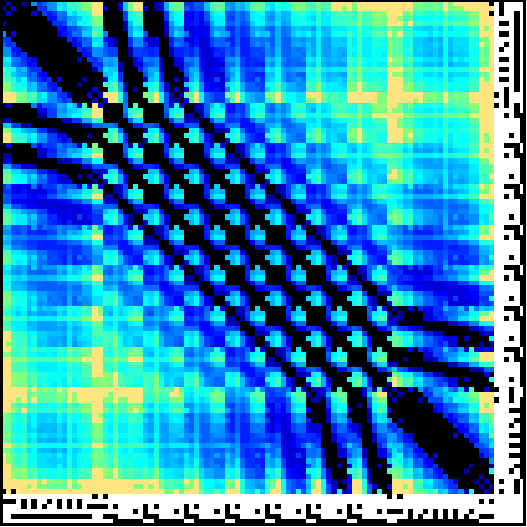
\includegraphics[width=\textwidth]{images/ch03/input-matrices/bddcml-benchmark/poc-8_4_2-1.pdf}
		\caption{\code{poisson\_on\_cube 8 4 2}}
		\label{Figure:comparing-decomposers-and-solvers->bddcml-benchmark->matrices-used-for-benchmarks->examples-of-element-patterns-in-matrices->8-4-2-1}
	\end{subfigure}%
	\hfill
	\begin{subfigure}[b]{0.48\textwidth}
		\centering
		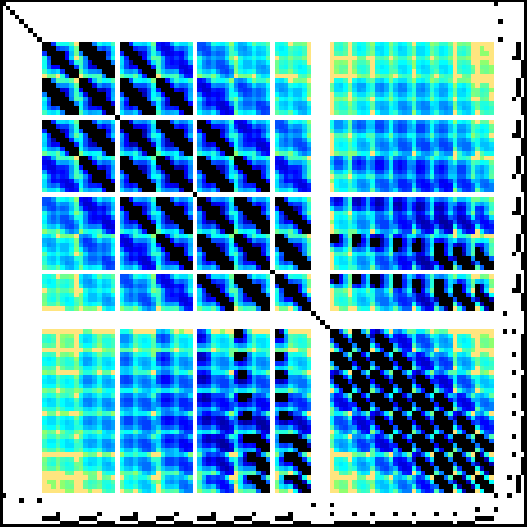
\includegraphics[width=\textwidth]{images/ch03/input-matrices/bddcml-benchmark/poc-8_4_2-2.pdf}
		\caption{\code{poisson\_on\_cube 8 4 2}}
		\label{Figure:comparing-decomposers-and-solvers->bddcml-benchmark->matrices-used-for-benchmarks->examples-of-element-patterns-in-matrices->8-4-2-2}
	\end{subfigure}
	
	\begin{subfigure}[b]{0.48\textwidth}
		\centering
		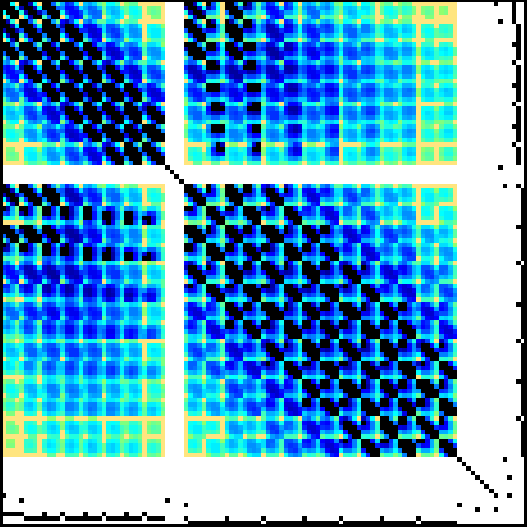
\includegraphics[width=\textwidth]{images/ch03/input-matrices/bddcml-benchmark/poc-8_4_2-3.pdf}
		\caption{\code{poisson\_on\_cube 8 4 2}}
		\label{Figure:comparing-decomposers-and-solvers->bddcml-benchmark->matrices-used-for-benchmarks->examples-of-element-patterns-in-matrices->8-4-2-3}
	\end{subfigure}%
	\hfill
	\begin{subfigure}[b]{0.48\textwidth}
		\centering
		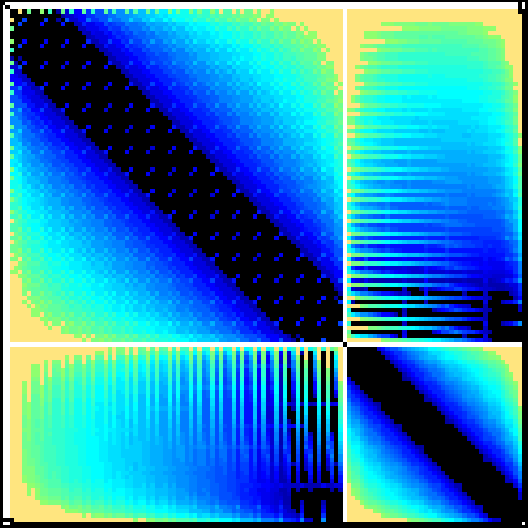
\includegraphics[width=\textwidth]{images/ch03/input-matrices/bddcml-benchmark/poc-32_4_2.pdf}
		\caption{\code{poisson\_on\_cube 32 4 2}}
		\label{Figure:comparing-decomposers-and-solvers->bddcml-benchmark->matrices-used-for-benchmarks->examples-of-element-patterns-in-matrices->32-4-2}
	\end{subfigure}
	
	\caption{Visualization of the nonzero element patterns in matrices encountered in the BDDCML benchmark.
		The captions indicate the configuration in which each matrix appeared.
	}
	\label{Figure:comparing-decomposers-and-solvers->bddcml-benchmark->matrices-used-for-benchmarks->examples-of-element-patterns-in-matrices}
\end{figure}

In Figure~\ref{Figure:comparing-decomposers-and-solvers->bddcml-benchmark->matrices-used-for-benchmarks->examples-of-element-patterns-in-matrices}, matrices with different element patterns can be observed in the same configuration: \code{poisson\_on\_cube 8 4 2}.
Furthermore, while the nonzero element pattern in Figure~\ref{Figure:comparing-decomposers-and-solvers->bddcml-benchmark->matrices-used-for-benchmarks->examples-of-element-patterns-in-matrices->32-4-2} appeared in \code{poisson\_on\_cube 32 4 2}, it seems to be a denser representation of the nonzero element pattern displayed in Figure~\ref{Figure:comparing-decomposers-and-solvers->bddcml-benchmark->matrices-used-for-benchmarks->examples-of-element-patterns-in-matrices->8-4-2-2}, which appeared in \code{poisson\_on\_cube 8 4 2}.



\subsection{Benchmark Results}\label{Subsection:comparing-decomposers-and-solvers->bddcml-benchmark->benchmark-results}
This section presents the benchmark results obtained by running the BDDCML benchmark using the decomposers listed in Table~\ref{Table:comparing-decomposers-and-solvers->bddcml-benchmark->benchmark-results->table-of-decomposers}, paired with the CuBLAStrsmPP solver (except for the MAGMA decomposer, which uses its own solver).
CuBLAStrsmPP was chosen as it supports the unit diagonal both in $\mathbf{L}$ and $\mathbf{U}$.

\begin{table}[ht!]
	\centering
	\begin{tabular}{|ll|c|c|}
		\hline
		\rowcolor[HTML]{C0C0C0} 
		\multicolumn{2}{|c|}{\cellcolor[HTML]{C0C0C0}\textbf{Decomposer}} & \cellcolor[HTML]{C0C0C0} & \multicolumn{1}{c|}{\cellcolor[HTML]{C0C0C0}} \\
		\rowcolor[HTML]{EFEFEF} 
		\multicolumn{1}{|c|}{\cellcolor[HTML]{EFEFEF}\textbf{Name}} & \multicolumn{1}{c|}{\cellcolor[HTML]{EFEFEF}\textbf{Abbreviation}} & \multirow{-2}{*}{\cellcolor[HTML]{C0C0C0}\textbf{Variants}} & \multicolumn{1}{c|}{\multirow{-2}{*}{\cellcolor[HTML]{C0C0C0}\textbf{Performer}}} \\ \hline
		\multicolumn{1}{|l|}{CuSolverDnXgetrf with Partial Piv.}         & CuSolverDnXgetrfPP &     -     &    GPU    \\
		\multicolumn{1}{|l|}{Iterative Crout's Method with Partial Piv.} & ICM\_\textit{x}PP  & 8, 16, 32 &    GPU    \\
		\multicolumn{1}{|l|}{magma\_dgetrf\_gpu}                         & MAGMAgetrf         &     -     & CPU + GPU \\
		\multicolumn{1}{|l|}{Parallel Crout's Method with Partial Piv.}  & PCM\_\textit{x}PP  & 8, 16, 32 &    GPU    \\ \hline
	\end{tabular}
	\caption{Decomposers compared in the benchmark: CuSolverDnXgetrfPP (mentioned in Section~\ref{Subsection:implementation->libraries-used->CUDA-libraries->cuSOLVER}), ICM\_\textit{x}PP (described in \namerefItalics{Paragraph:implementation->decomposition-project->implemented-solutions->decomposers->ICMxPP} in Section~\ref{Subsection:implementation->decomposition-project->implemented-solutions->decomposers}), MAGMAgetrf (description available in the MAGMA documentation\tablefootnote{MAGMA Documentation for getrf URL: \url{https://icl.utk.edu/projectsfiles/magma/doxygen/group__magma__getrf.html}}), and PCM\_\textit{x}PP (described in \namerefItalics{Paragraph:implementation->decomposition-project->implemented-solutions->decomposers->PCMxPP} in Section~\ref{Subsection:implementation->decomposition-project->implemented-solutions->decomposers}).
		The \textit{Variants} column indicates the different configurations of the decomposer.
		For example, ICM\_\textit{x}PP was benchmarked as three separate decomposers depending on the CUDA thread block configuration.
		In the case of PCM\_\textit{x}PP, the thread blocks are one-dimensional, and the number of threads per block is $x^2$.
		Unless stated otherwise, the processing tolerance for ICM\_\textit{x}PP was set to zero, and the lower bound and upper bound of conditional partial pivoting tolerance were set to \num{1e-5} and \num{1e+5}, respectively.
		For PCM\_\textit{x}PP, the conditional partial pivoting tolerance was set to \num{1e-5}.
		Note that the \code{magmaf\_dgetrf\_gpu()} function was already used in BDDCML prior to this thesis and it is not available in the Decomposition project.
		The \textit{Performer} column specifies the primary device used by each decomposer.
	}
	\label{Table:comparing-decomposers-and-solvers->bddcml-benchmark->benchmark-results->table-of-decomposers}
\end{table}

First, the speedup comparison in the \textit{Preconditioner Setup} stage between the baseline implementation in BDDCML, MAGMAgetrf, and the other decomposers listed in Table~\ref{Table:comparing-decomposers-and-solvers->bddcml-benchmark->benchmark-results->table-of-decomposers} is presented.
Then, a comparison of the highest-performing decomposers is provided.
Finally, the accuracy of the results is mentioned.


\subsubsection{Speedup Comparison of Decomposers in the Preconditioner Setup Stage}\label{Subsection:comparing-decomposers-and-solvers->bddcml-benchmark->benchmark-results->speedup-comparison-of-decomposers-in-pc-setup-stage}
This section presents the speedup comparison of the decomposers listed in Table~\ref{Table:comparing-decomposers-and-solvers->bddcml-benchmark->benchmark-results->table-of-decomposers} relative to MAGMAgetrf.
For clarity, the times discussed in this section represent the total time taken by the \textit{pc\_setup} stage.
Specifically, for each benchmark, the \code{poisson\_on\_cube} executable was run ten times for each value of $H/h$.
The recorded times from all runs were subsequently averaged and logged.
The speedup comparison is shown in Figure~\ref{Figure:comparing-decomposers-and-solvers->bddcml-benchmark->benchmark-results->speedup-comparison-of-decomposers-in-pc-setup-stage->speedup-comparison}.

\begin{figure}[ht!]
	\centering
	\tikzset{mark options={mark size=2.0, line width=0.5pt},font=\small}
	\begin{tikzpicture}
		\pgfplotstableread[col sep=comma]{resources/ch03/bddcml-benchmarks/decomposers_benchmark_results_5_to_50_allDecomposers.csv}\datatable
		\begin{axis}
			[
			,width=0.98\textwidth
			,height=0.45\textwidth
			,axis x line*=bottom
			,axis y line*=left
			,xlabel=\textbf{$H/h$}
			,ylabel=\textbf{Speedup rel. to MAGMAgetrf}
			,x label style={at={(axis description cs:0.46,-.1)}}
			,xmin=0, xmax=55
			,ymajorgrids
			,legend style={
				at={(0.5,1.025)},
				anchor=south,
				legend columns=4,
				/tikz/every even column/.append style={column sep=0.5cm},
				draw=black, % Remove legend border
				nodes={inner sep=3pt}, % Adjust the spacing between legend entries
				font=\small % Adjust the font size of the legend entries
			}
			]
			\addplot[black,mark=triangle*] table [x=Num. el. per sub-edge, y={MAGMAdgetrf_gpu - PC Setup Speedup rel. to MAGMAdgetrf_gpu}] {\datatable};
			\addlegendentry{MAGMAgetrf}
			\addplot[blue,mark=triangle*] table [x=Num. el. per sub-edge, y={ICM_8 PP - PC Setup Speedup rel. to MAGMAdgetrf_gpu}] {\datatable};
			\addlegendentry{ICM\_8PP}
			\addplot[purple,mark=triangle*] table [x=Num. el. per sub-edge, y={ICM_16 PP - PC Setup Speedup rel. to MAGMAdgetrf_gpu}] {\datatable};
			\addlegendentry{ICM\_16PP}
			\addplot[teal,mark=triangle*] table [x=Num. el. per sub-edge, y={ICM_32 PP - PC Setup Speedup rel. to MAGMAdgetrf_gpu}] {\datatable};
			\addlegendentry{ICM\_32PP}
			\addplot[green!60!black,mark=triangle*] table [x=Num. el. per sub-edge, y={CuSolverDnXgetrfWrapper PP - PC Setup Speedup rel. to MAGMAdgetrf_gpu}] {\datatable};
			\addlegendentry{CuSolverDnXgetrfPP}
			\addplot[red,mark=triangle*] table [x=Num. el. per sub-edge, y={PCM_8 PP - PC Setup Speedup rel. to MAGMAdgetrf_gpu}] {\datatable};
			\addlegendentry{PCM\_8PP}
			\addplot[green,mark=triangle*] table [x=Num. el. per sub-edge, y={PCM_16 PP - PC Setup Speedup rel. to MAGMAdgetrf_gpu}] {\datatable};
			\addlegendentry{PCM\_16PP}
			\addplot[cyan,mark=triangle*] table [x=Num. el. per sub-edge, y={PCM_32 PP - PC Setup Speedup rel. to MAGMAdgetrf_gpu}] {\datatable};
			\addlegendentry{PCM\_32PP}
		\end{axis}
	\end{tikzpicture}
	\caption{Speedup comparison of the \textit{pc\_setup} stage for the decomposers listed in Table~\ref{Table:comparing-decomposers-and-solvers->bddcml-benchmark->benchmark-results->table-of-decomposers} relative to MAGMAgetrf.}
	\label{Figure:comparing-decomposers-and-solvers->bddcml-benchmark->benchmark-results->speedup-comparison-of-decomposers-in-pc-setup-stage->speedup-comparison}
\end{figure}

As depicted in Figure~\ref{Figure:comparing-decomposers-and-solvers->bddcml-benchmark->benchmark-results->speedup-comparison-of-decomposers-in-pc-setup-stage->speedup-comparison}, the \textit{pc\_setup} stage was completed in the shortest time when either MAGMAgetrf or CuSolverDnXgetrfPP were used.
Specifically, with MAGMAgetrf, the execution of the stage was faster for smaller values of $H/h$, whereas for larger values, it was faster with CuSolverDnXgetrfPP.
In general, the use of the decomposers implemented by the author of this thesis resulted in the \textit{pc\_setup} stage taking longer to complete.
Out of the author's decomposers, ICM\_\textit{x}PP achieved the best performance.

\paragraph{ICM\_\textit{x}PP} The best-performing variant of ICM\_\textit{x}PP was ICM\_32PP.
Specifically, ICM\_32PP consistently outperformed ICM\_16PP, which in turn consistently outperformed ICM\_8PP.
This performance difference among the variants aligns with the results obtained by the variants of ICM\_\textit{x}PP in the Decomposition benchmark for decomposers, as mentioned on Page~\pageref{Text:comparing-decomposers-and-solvers->decomposition-project-benchmarks->decomposers-benchmark->comparison-of-execution-times-on-subset-of-matrices->ICMxPP->performance-of-variants}.
To further analyze ICM\_32PP, Figure~\ref{Figure:comparing-decomposers-and-solvers->bddcml-benchmark->benchmark-results->speedup-comparison-of-decomposers-in-pc-setup-stage->speedup-comparison->ICM_32PP->LU-and-metrics-examples} presents the \code{LU} matrices ICM\_32PP produced, along with its iterative and pivoting metrics for $H/h \in \left\{25, 50\right\}$.
The matrices presented in Figure~\ref{Figure:comparing-decomposers-and-solvers->bddcml-benchmark->benchmark-results->speedup-comparison-of-decomposers-in-pc-setup-stage->speedup-comparison->ICM_32PP->LU-and-metrics-examples} were chosen at random, as ICM\_32PP was called multiple times within each run of the \code{poisson\_on\_cube} executable.
Incidentally, the nonzero element pattern of both matrices was similar.

\begin{figure}[ht!]
	\centering
	\begin{subfigure}[t]{0.45\textwidth}
		\centering
		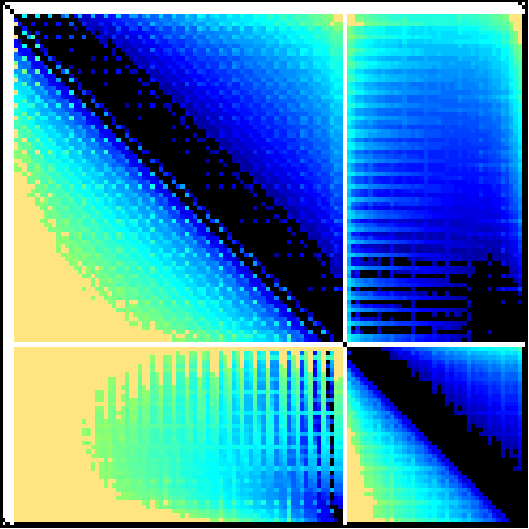
\includegraphics[width=\textwidth]{images/ch03/input-matrices/bddcml-benchmark/poc-25_4_2-LU_ICM32PP.pdf}
		\caption{Nonzero element pattern of the \code{LU} matrix produced by ICM\_32PP for a 1,964-by-1,964 matrix when $H/h$ was set to 25.}
		\label{Figure:comparing-decomposers-and-solvers->bddcml-benchmark->benchmark-results->speedup-comparison-of-decomposers-in-pc-setup-stage->speedup-comparison->ICM_32PP->25-4-2->LU}
	\end{subfigure}%
	\hspace{0.03\textwidth}
	\begin{subfigure}[t]{0.51\textwidth}
		\centering
		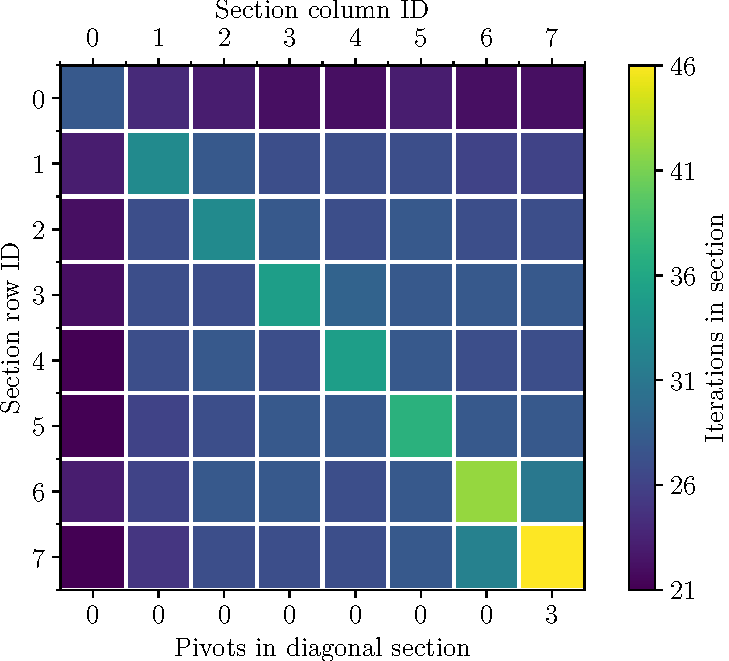
\includegraphics[width=\textwidth]{images/ch03/input-matrices/bddcml-benchmark/poc-25_4_2_icm32pp_metrics.pdf}
		\caption{Iterative and pivoting metrics of ICM\_32PP collected during the decomposition of a 1,964-by-1,964 matrix when $H/h$ was set to 25.
			Each square represents a 256-by-256 section of the matrix.
		}
		\label{Figure:comparing-decomposers-and-solvers->bddcml-benchmark->benchmark-results->speedup-comparison-of-decomposers-in-pc-setup-stage->speedup-comparison->ICM_32PP->25-4-2->metrics}
	\end{subfigure}
	
	\begin{subfigure}[t]{0.45\textwidth}
		\centering
		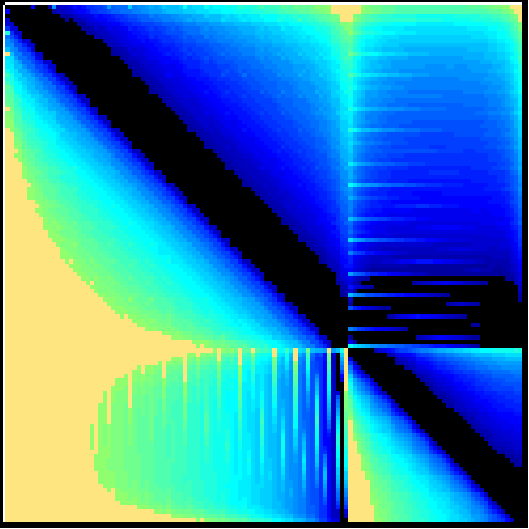
\includegraphics[width=\textwidth]{images/ch03/input-matrices/bddcml-benchmark/poc-50_4_2-LU_ICM32PP.pdf}
		\caption{Nonzero element pattern of the \code{LU} matrix produced by ICM\_32PP for a 7,664-by-7,664 matrix when $H/h$ was set to 50.}
		\label{Figure:comparing-decomposers-and-solvers->bddcml-benchmark->benchmark-results->speedup-comparison-of-decomposers-in-pc-setup-stage->speedup-comparison->ICM_32PP->50-4-2->LU}
	\end{subfigure}%
	\hspace{0.03\textwidth}
	\begin{subfigure}[t]{0.51\textwidth}
		\centering
		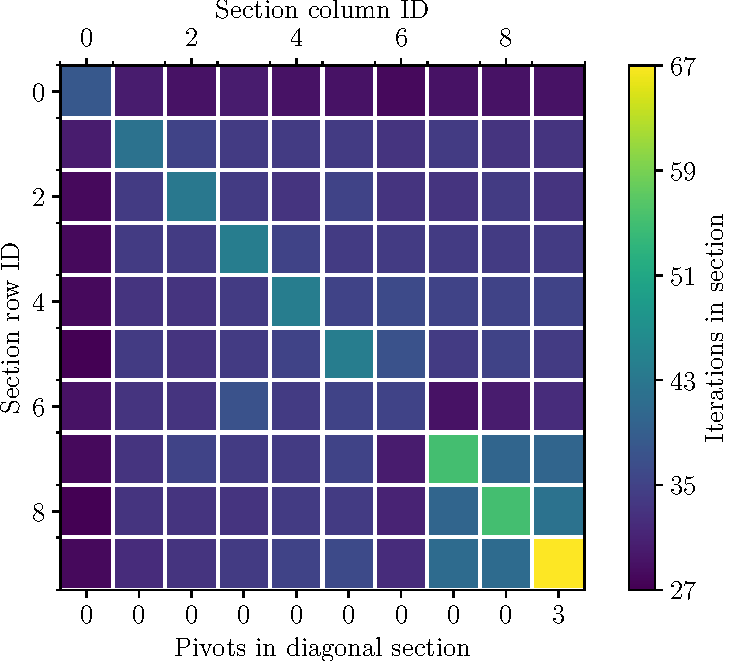
\includegraphics[width=\textwidth]{images/ch03/input-matrices/bddcml-benchmark/poc-50_4_2_icm32pp_metrics.pdf}
		\caption{Iterative and pivoting metrics of ICM\_32PP collected during the decomposition of a 7,664-by-7,664 matrix when $H/h$ was set to 50.
			Each square represents a 768-by-768 section of the matrix.
		}
		\label{Figure:comparing-decomposers-and-solvers->bddcml-benchmark->benchmark-results->speedup-comparison-of-decomposers-in-pc-setup-stage->speedup-comparison->ICM_32PP->50-4-2->metrics}
	\end{subfigure}

	\caption{Visualization of the nonzero element patterns of \code{LU} matrices produced by ICM\_32PP in the \textit{pc\_setup} stage for $H/h \in \left\{25, 50\right\}$.
		The figure includes the iterative and pivoting metrics of ICM\_32PP.
		In the \code{LU} plot, the color of nonzero elements depends on their absolute value.
		Small entries are light orange, large entries are black, and the color of mid-range entries ranges from light green to deep blue depending on the median of $\log_{10}$ of the nonzero values (with slight alterations) \cite{Davis2006}.
		The color of zero entries is white.
		In the metrics plot, the color in each square represents the number of iterations performed on that section.
		The left and top axes indicate the section ID in each dimension, and the bottom axis displays the number of pivots performed in a diagonal section.
	}
	\label{Figure:comparing-decomposers-and-solvers->bddcml-benchmark->benchmark-results->speedup-comparison-of-decomposers-in-pc-setup-stage->speedup-comparison->ICM_32PP->LU-and-metrics-examples}
\end{figure}

The iterative and pivoting metrics of ICM\_32PP presented in Figures~\ref{Figure:comparing-decomposers-and-solvers->bddcml-benchmark->benchmark-results->speedup-comparison-of-decomposers-in-pc-setup-stage->speedup-comparison->ICM_32PP->25-4-2->metrics} and \ref{Figure:comparing-decomposers-and-solvers->bddcml-benchmark->benchmark-results->speedup-comparison-of-decomposers-in-pc-setup-stage->speedup-comparison->ICM_32PP->50-4-2->metrics} indicate that the performance can be attributed to three factors:
%
\begin{tight_enumerate}
	\item Firstly, the initial estimate of \code{LU} (the input matrix) was suitable, as indicated by the lower number of iterations for sections with column and row IDs equal to 0.
However, the low number of iterations can also be attributed to the patches of zeros, as mentioned in the following point.
	\item Secondly, the matrices contained patches of zeros, which are known to reduce the number of iterations required to process sections.
For example, in Figure~\ref{Figure:comparing-decomposers-and-solvers->bddcml-benchmark->benchmark-results->speedup-comparison-of-decomposers-in-pc-setup-stage->speedup-comparison->ICM_32PP->50-4-2->metrics}, the sections below and to the right of section (6, 6) required fewer iterations compared to the surrounding sections, as they computed patches of zeros.
While the patches are not visible in Figure~\ref{Figure:comparing-decomposers-and-solvers->bddcml-benchmark->benchmark-results->speedup-comparison-of-decomposers-in-pc-setup-stage->speedup-comparison->ICM_32PP->50-4-2->LU} due to the matrix dimensions, they are visible in Figure~\ref{Figure:comparing-decomposers-and-solvers->bddcml-benchmark->benchmark-results->speedup-comparison-of-decomposers-in-pc-setup-stage->speedup-comparison->ICM_32PP->25-4-2->LU}, where the nonzero element pattern is similar.
	\item Thirdly, despite the matrices being dense, the individual sections did not require many iterations to be processed.
For example, approximately 86\% of the elements in the input matrix for $H/h = 25$ were nonzero, while for $H/h = 50$, the percentage increased to 92\%.
\end{tight_enumerate}

The summary of the decomposition benchmarks in Section~\ref{Subsection:comparing-decomposers-and-solvers->decomposition-project-benchmarks->solvers-benchmark->summary-of-results-of-decomposition-benchmarks} suggested that using a higher processing tolerance for ICM\_\textit{x}PP may be suitable when the decomposer is employed as a preconditioner that is not expected to be highly accurate.
As mentioned earlier on Page~\pageref{Text:comparing-decomposers-and-solvers->bddcml-benchmark->poisson-on-cube-stages}, the \textit{Krylov method} stage uses the \code{LU} matrices produced by the decomposer to iteratively improve the solution.
Hence, an inaccurate decomposition could potentially benefit the overall execution time of the problem.
To investigate this claim, ICM\_32PP with various processing tolerances was utilized as a decomposer in the \textit{pc\_setup} stage.
Only the ICM\_32PP variant is presented since it consistently outperformed the other variants of ICM\_\textit{x}PP.
Figure~\ref{Figure:comparing-decomposers-and-solvers->bddcml-benchmark->benchmark-results->speedup-comparison-of-decomposers-in-pc-setup-stage->speedup-comparison->ICMxPP-with-varying-processing-tolerances->speedup-comparison-relative-to-MAGMAgetrf} illustrates the speedups of ICM\_32PP with various processing tolerances relative to MAGMAgetrf.
Furthermore, the figure also displays the execution times of the \textit{pc\_setup} stage for ICM\_32PP with various processing tolerances and MAGMAgetrf.

\begin{figure}[ht!]
	\centering
	\tikzset{mark options={mark size=2.0, line width=0.5pt},font=\small}
	\begin{subfigure}{\textwidth}
		\begin{tikzpicture}
			\pgfplotstableread[col sep=comma]{resources/ch03/bddcml-benchmarks/decomposers_benchmark_results_5_to_50_allDecomposers.csv}\allDecomposersDatatable
			\pgfplotstableread[col sep=comma]{resources/ch03/bddcml-benchmarks/decomposers_benchmark_results_5_to_50_processing_tols_ICM_32PP.csv}\processingTolerancesDatatable
			\begin{axis}
				[
				,width=0.98\textwidth
				,height=0.45\textwidth
				,axis x line*=bottom
				,axis y line*=left
				,xlabel=\textbf{$H/h$}
				,ylabel=\textbf{Speedup rel. to MAGMAgetrf}
				,x label style={at={(axis description cs:0.46,-.1)}}
				,xmin=0, xmax=55
				,ymajorgrids
				,legend style={
					at={(0.5,1.025)},
					anchor=south,
					legend columns=3,
					/tikz/every even column/.append style={column sep=0.5cm},
					draw=black, % Remove legend border
					nodes={inner sep=3pt}, % Adjust the spacing between legend entries
					font=\small % Adjust the font size of the legend entries
				}
				]
				\addplot[black,mark=triangle*] table [x=Num. el. per sub-edge, y={MAGMAdgetrf_gpu - PC Setup Speedup rel. to MAGMAdgetrf_gpu}] {\allDecomposersDatatable};
				\addlegendentry{MAGMAgetrf}
				\addplot[teal,mark=triangle*] table [x=Num. el. per sub-edge, y={ICM_32 PP - PC Setup Speedup rel. to MAGMAdgetrf_gpu}] {\allDecomposersDatatable};
				\addlegendentry{ICM\_32PP 0}
				\addplot[red,mark=triangle*] table [x=Num. el. per sub-edge, y={ICM_32 PP 1e-10 - PC Setup Speedup rel. to MAGMAdgetrf_gpu}] {\processingTolerancesDatatable};
				\addlegendentry{ICM\_32 PP 1e-10}
				\addplot[cyan,mark=triangle*] table [x=Num. el. per sub-edge, y={ICM_32 PP 1e-05 - PC Setup Speedup rel. to MAGMAdgetrf_gpu}] {\processingTolerancesDatatable};
				\addlegendentry{ICM\_32 PP 1e-5}
				\addplot[green!60!black,mark=triangle*] table [x=Num. el. per sub-edge, y={ICM_32 PP 0.01 - PC Setup Speedup rel. to MAGMAdgetrf_gpu}] {\processingTolerancesDatatable};
				\addlegendentry{ICM\_32 PP 0.01}
				\addplot[blue,mark=triangle*] table [x=Num. el. per sub-edge, y={ICM_32 PP 0.1 - PC Setup Speedup rel. to MAGMAdgetrf_gpu}] {\processingTolerancesDatatable};
				\addlegendentry{ICM\_32 PP 0.1}
				\addplot[green,mark=triangle*] table [x=Num. el. per sub-edge, y={ICM_32 PP 0.2 - PC Setup Speedup rel. to MAGMAdgetrf_gpu}] {\processingTolerancesDatatable};
				\addlegendentry{ICM\_32 PP 0.2}
				\addplot[purple,mark=triangle*] table [x=Num. el. per sub-edge, y={ICM_32 PP 0.5 - PC Setup Speedup rel. to MAGMAdgetrf_gpu}] {\processingTolerancesDatatable};
				\addlegendentry{ICM\_32 PP 0.5}
				\addplot[orange,mark=triangle*] table [x=Num. el. per sub-edge, y={ICM_32 PP 1 - PC Setup Speedup rel. to MAGMAdgetrf_gpu}] {\processingTolerancesDatatable};
				\addlegendentry{ICM\_32 PP 1}
			\end{axis}
		\end{tikzpicture}
		\subcaption{Speedup relative to MAGMAgetrf}
		\label{Figure:comparing-decomposers-and-solvers->bddcml-benchmark->benchmark-results->speedup-comparison-of-decomposers-in-pc-setup-stage->speedup-comparison->ICMxPP-with-varying-processing-tolerances->speedup-comparison-relative-to-MAGMAgetrf}
	\end{subfigure}
	\begin{subfigure}{\textwidth}
		\begin{tikzpicture}
			\pgfplotstableread[col sep=comma]{resources/ch03/bddcml-benchmarks/decomposers_benchmark_results_5_to_50_allDecomposers.csv}\allDecomposersDatatable
			\pgfplotstableread[col sep=comma]{resources/ch03/bddcml-benchmarks/decomposers_benchmark_results_5_to_50_processing_tols_ICM_32PP.csv}\processingTolerancesDatatable
			\begin{axis}
				[
				,width=0.98\textwidth
				,height=0.45\textwidth
				,axis x line*=bottom
				,axis y line*=left
				,xlabel=\textbf{$H/h$}
				,ylabel=\textbf{\textit{pc\_setup} time [s]}
				,x label style={at={(axis description cs:0.46,-.1)}}
				,xmin=0, xmax=55
				,ymajorgrids
				]
				\addplot[black,mark=triangle*] table [x=Num. el. per sub-edge, y={MAGMAdgetrf_gpu - PC Setup Time [s]}] {\allDecomposersDatatable};
				\addplot[teal,mark=triangle*] table [x=Num. el. per sub-edge, y={ICM_32 PP - PC Setup Time [s]}] {\allDecomposersDatatable};
				\addplot[red,mark=triangle*] table [x=Num. el. per sub-edge, y={ICM_32 PP 1e-10 - PC Setup Time [s]}] {\processingTolerancesDatatable};
				\addplot[cyan,mark=triangle*] table [x=Num. el. per sub-edge, y={ICM_32 PP 1e-05 - PC Setup Time [s]}] {\processingTolerancesDatatable};
				\addplot[green!60!black,mark=triangle*] table [x=Num. el. per sub-edge, y={ICM_32 PP 0.01 - PC Setup Time [s]}] {\processingTolerancesDatatable};
				\addplot[blue,mark=triangle*] table [x=Num. el. per sub-edge, y={ICM_32 PP 0.1 - PC Setup Time [s]}] {\processingTolerancesDatatable};
				\addplot[green,mark=triangle*] table [x=Num. el. per sub-edge, y={ICM_32 PP 0.2 - PC Setup Time [s]}] {\processingTolerancesDatatable};
				\addplot[purple,mark=triangle*] table [x=Num. el. per sub-edge, y={ICM_32 PP 0.5 - PC Setup Time [s]}] {\processingTolerancesDatatable};
				\addplot[orange,mark=triangle*] table [x=Num. el. per sub-edge, y={ICM_32 PP 1 - PC Setup Time [s]}] {\processingTolerancesDatatable};
			\end{axis}
		\end{tikzpicture}
		\subcaption{Execution times}
		\label{Figure:comparing-decomposers-and-solvers->bddcml-benchmark->benchmark-results->speedup-comparison-of-decomposers-in-pc-setup-stage->speedup-comparison->ICMxPP-with-varying-processing-tolerances->pc-setup-time-with-MAGMAgetrf}
	\end{subfigure}
	\caption{Speedup comparison of the \textit{pc\_setup} stage for ICM\_32PP with various processing tolerances relative to MAGMAgetrf.
		The execution times of the stage are included for context.
		The name of each ICM\_32PP decomposer follows the naming pattern \textit{decomposer <processing\_tolerance>}.
	}
	\label{Figure:comparing-decomposers-and-solvers->bddcml-benchmark->benchmark-results->speedup-comparison-of-decomposers-in-pc-setup-stage->speedup-comparison->ICMxPP-with-varying-processing-tolerances->speedup-comparison-relative-to-MAGMAgetrf-and-pc-setup-execution-time}
\end{figure}

As depicted in Figure~\ref{Figure:comparing-decomposers-and-solvers->bddcml-benchmark->benchmark-results->speedup-comparison-of-decomposers-in-pc-setup-stage->speedup-comparison->ICMxPP-with-varying-processing-tolerances->speedup-comparison-relative-to-MAGMAgetrf-and-pc-setup-execution-time}, increasing the processing tolerance of ICM\_32PP resulted in  improved performance.
For example, with $H/h$ set to 50, "ICM\_32PP 1" achieved a speedup of 0.92 relative to MAGMAgetrf.
It is worth noting that larger processing tolerances were not explored, as the performance gains between tolerances 0.5 and 1 were minimal, as shown in Figure~\ref{Figure:comparing-decomposers-and-solvers->bddcml-benchmark->benchmark-results->speedup-comparison-of-decomposers-in-pc-setup-stage->speedup-comparison->ICMxPP-with-varying-processing-tolerances->speedup-comparison-relative-to-MAGMAgetrf}.

However, as described on Page~\pageref{Text:comparing-decomposers-and-solvers->decomposition-project-benchmarks->decomposers-benchmark->accuracy-of-results-on-all-matrices->double-precision->ICM32PP->various-processing-tolerances->description-of-figure-with-accuracy-results}, increasing the processing tolerance results in lower accuracy of the results.
This decrease in accuracy is observed in the \textit{Krylov method} stage, where the matrices produced by ICM\_32PP are used.
Specifically, a higher number of iterations are needed to achieve the desired accuracy of the solution, consequently leading to longer execution times of the stage.
Figure~\ref{Figure:comparing-decomposers-and-solvers->bddcml-benchmark->benchmark-results->speedup-comparison-of-decomposers-in-pc-setup-stage->speedup-comparison->ICMxPP-with-varying-processing-tolerances->krylov-method-iterations-and-time-with-MAGMAgetrf} presents the number of iterations and the execution times of the \textit{Krylov method} stage for ICM\_32PP with various processing tolerances, as well as for MAGMAgetrf.

\begin{figure}[ht!]
	\centering
	\tikzset{mark options={mark size=2.0, line width=0.5pt},font=\small}
	\begin{subfigure}{\textwidth}
		\begin{tikzpicture}
			\pgfplotstableread[col sep=comma]{resources/ch03/bddcml-benchmarks/decomposers_benchmark_results_5_to_50_allDecomposers.csv}\allDecomposersDatatable
			\pgfplotstableread[col sep=comma]{resources/ch03/bddcml-benchmarks/decomposers_benchmark_results_5_to_50_processing_tols_ICM_32PP.csv}\processingTolerancesDatatable
			\begin{axis}
				[
				,width=0.98\textwidth
				,height=0.45\textwidth
				,axis x line*=bottom
				,axis y line*=left
				,xlabel=\textbf{$H/h$}
				,ylabel=\textbf{\textit{Krylov method} iterations}
				,x label style={at={(axis description cs:0.46,-.1)}}
				,xmin=0, xmax=55
				,ymajorgrids
				,legend style={
					at={(0.5,1.025)},
					anchor=south,
					legend columns=3,
					/tikz/every even column/.append style={column sep=0.5cm},
					draw=black, % Remove legend border
					nodes={inner sep=3pt}, % Adjust the spacing between legend entries
					font=\small % Adjust the font size of the legend entries
				}
				]
				\addplot[black,mark=triangle*] table [x=Num. el. per sub-edge, y={MAGMAdgetrf_gpu - Krylov PCG num. iters.}] {\allDecomposersDatatable};
				\addlegendentry{MAGMAgetrf}
				\addplot[teal,mark=triangle*] table [x=Num. el. per sub-edge, y={ICM_32 PP - Krylov PCG num. iters.}] {\allDecomposersDatatable};
				\addlegendentry{ICM\_32PP 0}
				\addplot[red,mark=triangle*] table [x=Num. el. per sub-edge, y={ICM_32 PP 1e-10 - Krylov PCG num. iters.}] {\processingTolerancesDatatable};
				\addlegendentry{ICM\_32 PP 1e-10}
				\addplot[cyan,mark=triangle*] table [x=Num. el. per sub-edge, y={ICM_32 PP 1e-05 - Krylov PCG num. iters.}] {\processingTolerancesDatatable};
				\addlegendentry{ICM\_32 PP 1e-5}
				\addplot[green!60!black,mark=triangle*] table [x=Num. el. per sub-edge, y={ICM_32 PP 0.01 - Krylov PCG num. iters.}] {\processingTolerancesDatatable};
				\addlegendentry{ICM\_32 PP 0.01}
				\addplot[blue,mark=triangle*] table [x=Num. el. per sub-edge, y={ICM_32 PP 0.1 - Krylov PCG num. iters.}] {\processingTolerancesDatatable};
				\addlegendentry{ICM\_32 PP 0.1}
				\addplot[green,mark=triangle*] table [x=Num. el. per sub-edge, y={ICM_32 PP 0.2 - Krylov PCG num. iters.}] {\processingTolerancesDatatable};
				\addlegendentry{ICM\_32 PP 0.2}
				\addplot[purple,mark=triangle*] table [x=Num. el. per sub-edge, y={ICM_32 PP 0.5 - Krylov PCG num. iters.}] {\processingTolerancesDatatable};
				\addlegendentry{ICM\_32 PP 0.5}
				\addplot[orange,mark=triangle*] table [x=Num. el. per sub-edge, y={ICM_32 PP 1 - Krylov PCG num. iters.}] {\processingTolerancesDatatable};
				\addlegendentry{ICM\_32 PP 1}
			\end{axis}
		\end{tikzpicture}
		\subcaption{Number of iterations}
		\label{Figure:comparing-decomposers-and-solvers->bddcml-benchmark->benchmark-results->speedup-comparison-of-decomposers-in-pc-setup-stage->speedup-comparison->ICMxPP-with-varying-processing-tolerances->krylov-method-iterations-and-time-with-MAGMAgetrf->iterations}
	\end{subfigure}
	\begin{subfigure}{\textwidth}
		\begin{tikzpicture}
			\pgfplotstableread[col sep=comma]{resources/ch03/bddcml-benchmarks/decomposers_benchmark_results_5_to_50_allDecomposers.csv}\allDecomposersDatatable
			\pgfplotstableread[col sep=comma]{resources/ch03/bddcml-benchmarks/decomposers_benchmark_results_5_to_50_processing_tols_ICM_32PP.csv}\processingTolerancesDatatable
			\begin{axis}
				[
				,width=0.98\textwidth
				,height=0.45\textwidth
				,axis x line*=bottom
				,axis y line*=left
				,xlabel=\textbf{$H/h$}
				,ylabel=\textbf{\textit{Krylov method} time [s]}
				,x label style={at={(axis description cs:0.46,-.1)}}
				,xmin=0, xmax=55
				,ymajorgrids
				]
				\addplot[black,mark=triangle*] table [x=Num. el. per sub-edge, y={MAGMAdgetrf_gpu - Krylov Method Time [s]}] {\allDecomposersDatatable};
				\addplot[teal,mark=triangle*] table [x=Num. el. per sub-edge, y={ICM_32 PP - Krylov Method Time [s]}] {\allDecomposersDatatable};
				\addplot[red,mark=triangle*] table [x=Num. el. per sub-edge, y={ICM_32 PP 1e-10 - Krylov Method Time [s]}] {\processingTolerancesDatatable};
				\addplot[cyan,mark=triangle*] table [x=Num. el. per sub-edge, y={ICM_32 PP 1e-05 - Krylov Method Time [s]}] {\processingTolerancesDatatable};
				\addplot[green!60!black,mark=triangle*] table [x=Num. el. per sub-edge, y={ICM_32 PP 0.01 - Krylov Method Time [s]}] {\processingTolerancesDatatable};
				\addplot[blue,mark=triangle*] table [x=Num. el. per sub-edge, y={ICM_32 PP 0.1 - Krylov Method Time [s]}] {\processingTolerancesDatatable};
				\addplot[green,mark=triangle*] table [x=Num. el. per sub-edge, y={ICM_32 PP 0.2 - Krylov Method Time [s]}] {\processingTolerancesDatatable};
				\addplot[purple,mark=triangle*] table [x=Num. el. per sub-edge, y={ICM_32 PP 0.5 - Krylov Method Time [s]}] {\processingTolerancesDatatable};
				\addplot[orange,mark=triangle*] table [x=Num. el. per sub-edge, y={ICM_32 PP 1 - Krylov Method Time [s]}] {\processingTolerancesDatatable};
			\end{axis}
		\end{tikzpicture}
		\subcaption{Execution times (in seconds)}
		\label{Figure:comparing-decomposers-and-solvers->bddcml-benchmark->benchmark-results->speedup-comparison-of-decomposers-in-pc-setup-stage->speedup-comparison->ICMxPP-with-varying-processing-tolerances->krylov-method-iterations-and-time-with-MAGMAgetrf->time}
	\end{subfigure}
	\caption{Number of iterations and execution times of the \textit{Krylov method} stage for ICM\_32PP with various processing tolerances and MAGMAgetrf.
		The name of each ICM\_32PP decomposer follows the naming pattern \textit{decomposer <processing\_tolernace>}.
	}
	\label{Figure:comparing-decomposers-and-solvers->bddcml-benchmark->benchmark-results->speedup-comparison-of-decomposers-in-pc-setup-stage->speedup-comparison->ICMxPP-with-varying-processing-tolerances->krylov-method-iterations-and-time-with-MAGMAgetrf}
\end{figure}

As expected, Figure~\ref{Figure:comparing-decomposers-and-solvers->bddcml-benchmark->benchmark-results->speedup-comparison-of-decomposers-in-pc-setup-stage->speedup-comparison->ICMxPP-with-varying-processing-tolerances->krylov-method-iterations-and-time-with-MAGMAgetrf->iterations} demonstrates that the number of iterations in the \textit{Krylov method} stage increases as the processing tolerance values in ICM\_32PP rise.
However, as depicted in Figure~\ref{Figure:comparing-decomposers-and-solvers->bddcml-benchmark->benchmark-results->speedup-comparison-of-decomposers-in-pc-setup-stage->speedup-comparison->ICMxPP-with-varying-processing-tolerances->krylov-method-iterations-and-time-with-MAGMAgetrf->time}, the corresponding execution times of the stage, while increasing, remain relatively small compared to those of the \textit{pc\_setup} stage.
Consequently, the time saved by utilizing ICM\_32PP with a high processing tolerance in the \textit{pc\_setup} stage far outweighs the time lost in the \textit{Krylov method} stage due to the inaccurate results produced by the decomposer.

\subsubsection{Comparison of the Highest-Performing Variants} For completeness, Figure~\ref{Figure:comparing-decomposers-and-solvers->bddcml-benchmark->benchmark-results->speedup-comparison-of-decomposers-in-pc-setup-stage->speedup-comparison->best-variants->problem-total-time-with-MAGMAgetrf} displays the speedup comparison of the best-performing variants, including the various processing tolerances, of each decomposer listed in Table~\ref{Table:comparing-decomposers-and-solvers->bddcml-benchmark->benchmark-results->table-of-decomposers}, compared to MAGMAgetrf on the "Poisson equation on a cube" problem.

\begin{figure}[ht!]
	\centering
	\tikzset{mark options={mark size=2.0, line width=0.5pt},font=\small}
	\begin{tikzpicture}
		\pgfplotstableread[col sep=comma]{resources/ch03/bddcml-benchmarks/decomposers_benchmark_results_5_to_50_allDecomposers.csv}\allDecomposersDatatable
		\pgfplotstableread[col sep=comma]{resources/ch03/bddcml-benchmarks/decomposers_benchmark_results_5_to_50_processing_tols_ICM_32PP.csv}\processingTolerancesDatatable
		\begin{axis}
			[
			,width=0.98\textwidth
			,height=0.45\textwidth
			,axis x line*=bottom
			,axis y line*=left
			,xlabel=\textbf{$H/h$}
			,ylabel=\textbf{Speedup rel. to MAGMAgetrf}
			,x label style={at={(axis description cs:0.46,-.1)}}
			,xmin=0, xmax=55
			,ymax=1.2
			,ymajorgrids
			,legend style={
				at={(0.5,1.05)},
				anchor=south,
				legend columns=4,
				/tikz/every even column/.append style={column sep=0.5cm},
				draw=black, % Remove legend border
				nodes={inner sep=3pt}, % Adjust the spacing between legend entries
				font=\small % Adjust the font size of the legend entries
			}
			]
			\addplot[black,mark=triangle*] table [x=Num. el. per sub-edge, y={MAGMAdgetrf_gpu - PC Setup Speedup rel. to MAGMAdgetrf_gpu}] {\allDecomposersDatatable};
			\addlegendentry{MAGMAgetrf}
			\addplot[green!60!black,mark=triangle*] table [x=Num. el. per sub-edge, y={CuSolverDnXgetrfWrapper PP - PC Setup Speedup rel. to MAGMAdgetrf_gpu}] {\allDecomposersDatatable};
			\addlegendentry{CuSolverDnXgetrfPP}
			\addplot[teal,mark=triangle*] table [x=Num. el. per sub-edge, y={PCM_32 PP - PC Setup Speedup rel. to MAGMAdgetrf_gpu}] {\allDecomposersDatatable};
			\addlegendentry{PCM\_32PP}
			\addplot[orange,mark=triangle*] table [x=Num. el. per sub-edge, y={ICM_32 PP 1 - PC Setup Speedup rel. to MAGMAdgetrf_gpu}] {\processingTolerancesDatatable};
			\addlegendentry{ICM\_32 PP 1}
		\end{axis}
	\end{tikzpicture}
	\caption{Speedup comparison of the best-performing variants, including the various processing tolerances, of each decomposer listed in Table~\ref{Table:comparing-decomposers-and-solvers->bddcml-benchmark->benchmark-results->table-of-decomposers}, relative to MAGMAgetrf on the "Poisson equation on a cube" problem.}
	\label{Figure:comparing-decomposers-and-solvers->bddcml-benchmark->benchmark-results->speedup-comparison-of-decomposers-in-pc-setup-stage->speedup-comparison->best-variants->problem-total-time-with-MAGMAgetrf}
\end{figure}

As depicted in Figure~\ref{Figure:comparing-decomposers-and-solvers->bddcml-benchmark->benchmark-results->speedup-comparison-of-decomposers-in-pc-setup-stage->speedup-comparison->best-variants->problem-total-time-with-MAGMAgetrf}, overall, the "Poisson equation on a cube" problem was completed the fastest when CuSolverDnXgetrfPP was used along with CuBLAStrsmPP as the solver.
Its performance was followed by MAGMAgetrf, and ICM\_32PP 1 (with CuBLAStrsmPP as the solver).

\subsubsection{Accuracy of Results} The accuracy of results in the BDDCML benchmark was evaluated based on the number of iterations required in the \textit{Krylov method} stage.
However, excluding ICM\_\textit{x}PP with increased processing tolerances, the number of iterations was the same for all decomposers across all values of $H/h$.
In other words, the number of iterations for all decomposers listed in Table~\ref{Table:comparing-decomposers-and-solvers->bddcml-benchmark->benchmark-results->table-of-decomposers} matched that of MAGMAgetrf in Figure~\ref{Figure:comparing-decomposers-and-solvers->bddcml-benchmark->benchmark-results->speedup-comparison-of-decomposers-in-pc-setup-stage->speedup-comparison->ICMxPP-with-varying-processing-tolerances->krylov-method-iterations-and-time-with-MAGMAgetrf->iterations}.




\section{TNL Time-Series Problem Benchmark}\label{Section:comparing-decomposers-and-solvers->tnl-time-series-problem-benchmark}
During the development of the project, a hypothesis was formulated by doc. Ing. T. Oberhuber, Ph.D., that the initial estimate in ICM\_\textit{x}PP could be beneficial for time-series problems.
Specifically, it was proposed that the \code{LU} matrix from the previous time step could be used as an initial estimate in ICM\_\textit{x}PP for the current time step, potentially reducing the number of iterations needed to process the matrix.
This hypothesis was based on the observation that the input matrices undergo only slight changes between consecutive time steps, suggesting that the decomposed matrices may require fewer iterations to process.

For this purpose, doc. Ing. T. Oberhuber, Ph.D. implemented a benchmark for \textit{Mean curvature flow}\footnote{Mean curvature flow on Wikipedia: \url{https://en.wikipedia.org/wiki/Mean_curvature_flow}} in TNL\footnote{Mean curvature flow benchmark in TNL: \url{https://gitlab.com/tnl-project/tnl/-/tree/TO/grid/src/Benchmarks/MeanCurvatureFlow}}.
The benchmark specifically focused on ICM\_\textit{x}PP and aimed to determine whether using the \code{LU} matrix from the previous time step as the initial estimate would improve performance compared to using the default initial estimate (the input matrix).
Surprisingly, the benchmark results revealed no discernible difference in performance between the two approaches.
Therefore, the benchmark results are not presented in this thesis.
The reason behind the lack of difference remains unclear.
However, it offers an interesting area for further investigation in future research.




\section{Summary of Comparisons}\label{Section:comparing-decomposers-and-solvers->summary-of-comparisons}
This section summarizes the results of the benchmarks performed for the decomposers and solvers available in the Decomposition project.

Overall, the best-performing decomposer was CuSolverDnXgetrfPP, as it exhibited superior performance in both execution speed and accuracy in every benchmark it was a part of.
When considering the decomposers implemented by the author of this thesis, PCM\_\textit{x}PP demonstrated consistent performance with an acceptable level of accuracy.
However, for problems that require a preconditioner that does not need to produce highly accurate results, ICM\_\textit{x}PP is a suitable alternative.
It is important to note that increasing the processing tolerance of ICM\_\textit{x}PP can lead to higher performance, however, there is no guarantee that it will produce usable results.

In terms of solvers, both CuSolverDnXgetrsPP and CuBLAStrsmPP were the best-performing, with the former being marginally faster than the latter while being slightly less accurate.
It is worth noting that CuBLAStrsmPP allows for the unit diagonal to be stored either in \code{L} or \code{U}, whereas CuSolverDnXgetrsPP only supports a unit diagonal in \code{L}.
While IS\_\textit{x}PP demonstrated that its iterative approach can avoid unnecessary calculations in certain problems, it produced invalid results for others, even with its processing tolerance set to zero.
Therefore, it is not recommended for use.